% =============================================================================
%  Jungle Rest Stop - Computer Graphics Lab Project Report
%  Build:  pdflatex report.tex   (run twice for the table of contents)
%  Figures: main.exe --shots report/shots  ->  python report/make_figures.py
% =============================================================================
\documentclass[11pt,a4paper]{article}
\usepackage[margin=2.1cm]{geometry}
\usepackage[T1]{fontenc}
\usepackage{lmodern}
\usepackage{graphicx,float,caption,subcaption,booktabs,tabularx,longtable,array}
\usepackage{amsmath,amssymb}
\usepackage{xcolor,listings,enumitem,fancyhdr,parskip}
\usepackage{tikz}
\usetikzlibrary{arrows.meta,positioning,shapes.geometric,calc,fit,backgrounds}
\usepackage[hidelinks]{hyperref}
\usepackage[capitalise,noabbrev]{cleveref}

\newcommand{\studentname}{Md.\ Nayeem}
\newcommand{\studentroll}{2107050}
\newcommand{\coursename}{Computer Graphics and Image Processing Laboratory}
\newcommand{\coursecode}{CSE 4102}
\newcommand{\university}{Khulna University of Engineering \& Technology}
\newcommand{\department}{Department of Computer Science and Engineering}

\newcommand{\statStaticInstances}{85,721}
\newcommand{\statChunks}{101}
\newcommand{\statStaticLights}{36}
\newcommand{\statColliders}{1,590}
\newcommand{\statJungleTrees}{802}
\newcommand{\statPalms}{277}
\newcommand{\statBamboo}{137}
\newcommand{\statBushes}{1,532}
\newcommand{\statFerns}{2,174}
\newcommand{\statGrass}{4,680}
\newcommand{\statRocks}{200}
\newcommand{\statLogs}{84}
\newcommand{\statBuildSeconds}{0.65}

\newcommand{\svCube}{24}\newcommand{\stCube}{12}
\newcommand{\svCylinder}{102}\newcommand{\stCylinder}{96}
\newcommand{\svCylinderLow}{38}\newcommand{\stCylinderLow}{32}
\newcommand{\svSphere}{315}\newcommand{\stSphere}{560}
\newcommand{\svSphereLow}{54}\newcommand{\stSphereLow}{80}
\newcommand{\svCone}{64}\newcommand{\stCone}{60}
\newcommand{\svTruncatedCone}{86}\newcommand{\stTruncatedCone}{80}
\newcommand{\svTorus}{319}\newcommand{\stTorus}{560}
\newcommand{\svHemisphere}{211}\newcommand{\stHemisphere}{340}
\newcommand{\svWedge}{18}\newcommand{\stWedge}{8}
\newcommand{\svTaperedBox}{24}\newcommand{\stTaperedBox}{12}
\newcommand{\svQuad}{4}\newcommand{\stQuad}{2}
\newcommand{\svCrossCard}{8}\newcommand{\stCrossCard}{4}
\newcommand{\svLeafCard}{12}\newcommand{\stLeafCard}{6}
\newcommand{\svCoil}{606}\newcommand{\stCoil}{1200}

\graphicspath{{figures/}}
\setlength{\parskip}{0.55em}
\captionsetup{font=small,labelfont=bf}
\setlist{itemsep=0.15em,topsep=0.3em}

\definecolor{codebg}{RGB}{246,247,250}
\definecolor{codekw}{RGB}{0,70,160}
\definecolor{codecm}{RGB}{90,120,90}
\lstset{language=C++,basicstyle=\ttfamily\footnotesize,keywordstyle=\color{codekw}\bfseries,
  commentstyle=\color{codecm}\itshape,backgroundcolor=\color{codebg},frame=single,rulecolor=\color{black!15},
  breaklines=true,columns=fullflexible,showstringspaces=false,xleftmargin=0.6em,xrightmargin=0.6em}

\pagestyle{fancy}
\fancyhf{}
\cfoot{\thepage}
\renewcommand{\headrulewidth}{0pt}

\tikzset{
  box/.style={draw,rounded corners=3pt,align=center,fill=#1,minimum height=0.9cm,inner sep=4pt,font=\small},
  box/.default=blue!8,
  state/.style={draw,rounded corners=6pt,align=center,fill=#1,minimum height=0.8cm,inner sep=4pt,font=\small},
  state/.default=green!10,
  arr/.style={-{Stealth[length=2.5mm]},thick},
  lbl/.style={font=\footnotesize,midway,fill=white,inner sep=1pt}
}

\newcolumntype{P}[1]{>{\raggedright\arraybackslash}p{#1}}
% colour swatch and texture swatch used inside tables
\newcommand{\sw}[1]{{\setlength{\fboxsep}{0pt}\setlength{\fboxrule}{0.3pt}\fcolorbox[rgb]{0.55,0.55,0.55}{#1}{\rule{0pt}{0.7em}\rule{0.7em}{0pt}}}\,}
\newcommand{\txs}[1]{\raisebox{-0.2em}{\includegraphics[height=0.95em]{tx_#1}}}
\newcommand{\shot}[3][0.9]{\begin{figure}[H]\centering\includegraphics[width=#1\linewidth]{#2}\caption{#3}\end{figure}}
% object presentation: (a) complete | (b) disconnected parts with names, then the
% table of basic shapes and the table of every part with its transformation
\newcommand{\objviews}[3][8.2cm]{\begin{figure}[H]\centering\includegraphics[width=\linewidth,height=#1,keepaspectratio]{split_#2}\caption{#3}\label{fig:split_#2}\end{figure}%
\input{generated/shapes_#2.tex}\input{generated/pdet_#2.tex}}
\newcommand{\objhead}[1]{\par\smallskip\noindent\textbf{#1}\quad}

\begin{document}

% =============================================================================
\begin{titlepage}
\centering
\vspace*{0.6cm}
{\large \university\par}
{\normalsize \department\par}
\vspace{1.1cm}
{\Large \coursename\par}
{\large Course code: \coursecode\par}
\vspace{1.0cm}
{\Huge\bfseries Jungle Rest Stop\par}
\vspace{0.35cm}
{\Large An interactive 3D scene built only from basic shapes with OpenGL 3.3\\[0.15cm]
\large with vending machine, ATM, coffee machine \& library\par}
\vspace{0.9cm}
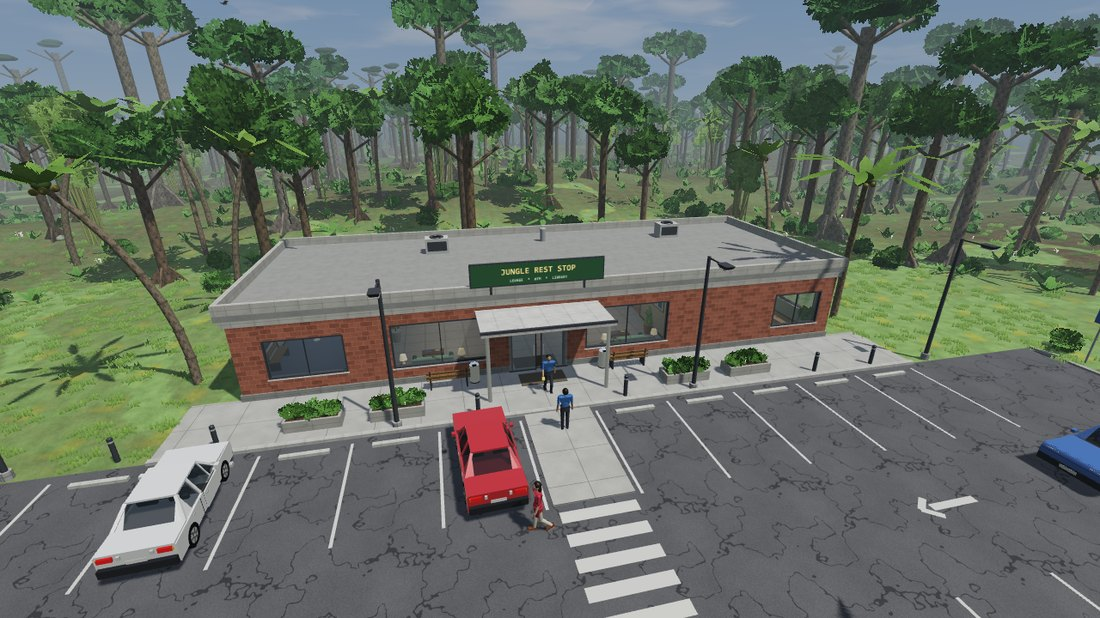
\includegraphics[width=0.84\linewidth]{ext_day}\par
\vspace{1.0cm}
\renewcommand{\arraystretch}{1.25}
\begin{tabular}{|P{7.4cm}|P{7.4cm}|}
\hline
\textbf{Submitted by} & \textbf{Submitted to} \\ \hline
\studentname \newline Roll: \studentroll \newline \department \newline \university
&
Md Tajmilur Rahman \newline Lecturer, Dept.\ of CSE, KUET \par\smallskip
Md.\ Mubtashim Abrar Nihal \newline Lecturer, Dept.\ of CSE, KUET \\ \hline
\end{tabular}
\par\vspace{0.8cm}
{\large Submission Date: 12 October 2026\par}
\vfill
\end{titlepage}

% =============================================================================
\tableofcontents
\newpage

% =============================================================================
\section{Introduction}
\emph{Jungle Rest Stop} is a real-time 3D scene made with OpenGL 3.3: a rest stop with a lounge, an ATM room
and a library in a jungle clearing. The user walks around and operates the vending machines, the ATM and the
coffee machine, while visitors arrive by car and use them too. Every object is built only from basic shapes
placed with translation, rotation and scaling; no model or image files are loaded.

% =============================================================================
\section{Overview of the Scene}\label{sec:tour}
\newcommand{\IntroW}{0.97}
\begin{figure}[H]\centering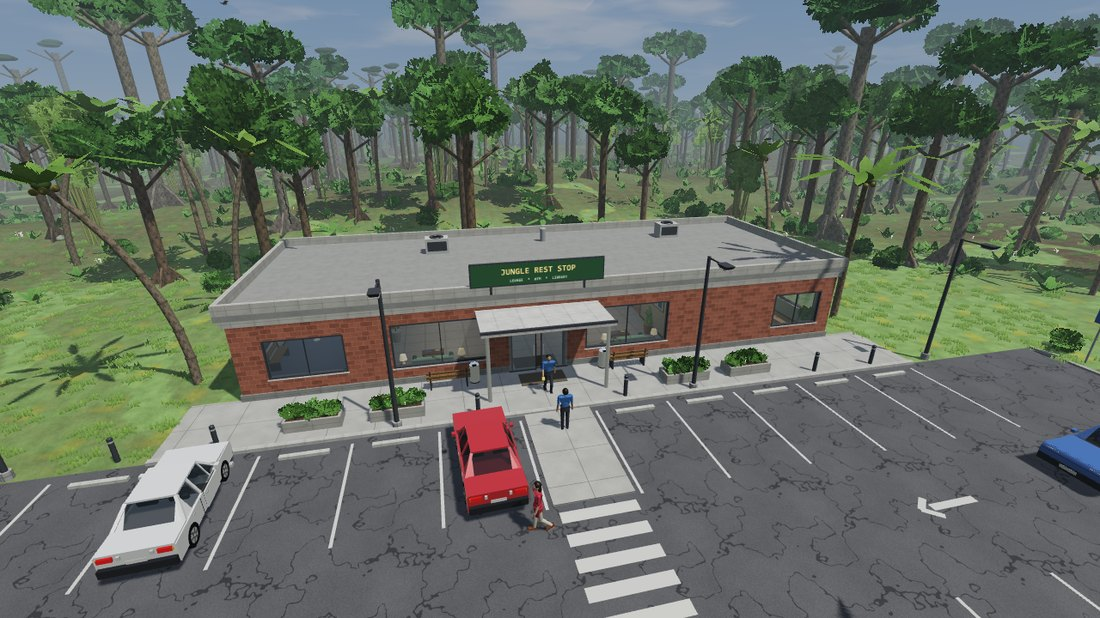
\includegraphics[width=\IntroW\linewidth]{ext_day}\caption{The rest stop by day: building, sidewalk, parking lot and street lamps.}\label{fig:extday}\end{figure}
\shot[\IntroW]{tour_lounge}{The main lounge: sofas, TV wall, coffee counter and the three vending machines.}
\shot[0.86]{tour_vending}{The three vending machines: cold drinks, crispy snacks and sweet treats.}
\begin{figure}[H]
\centering
\begin{subfigure}{0.49\linewidth}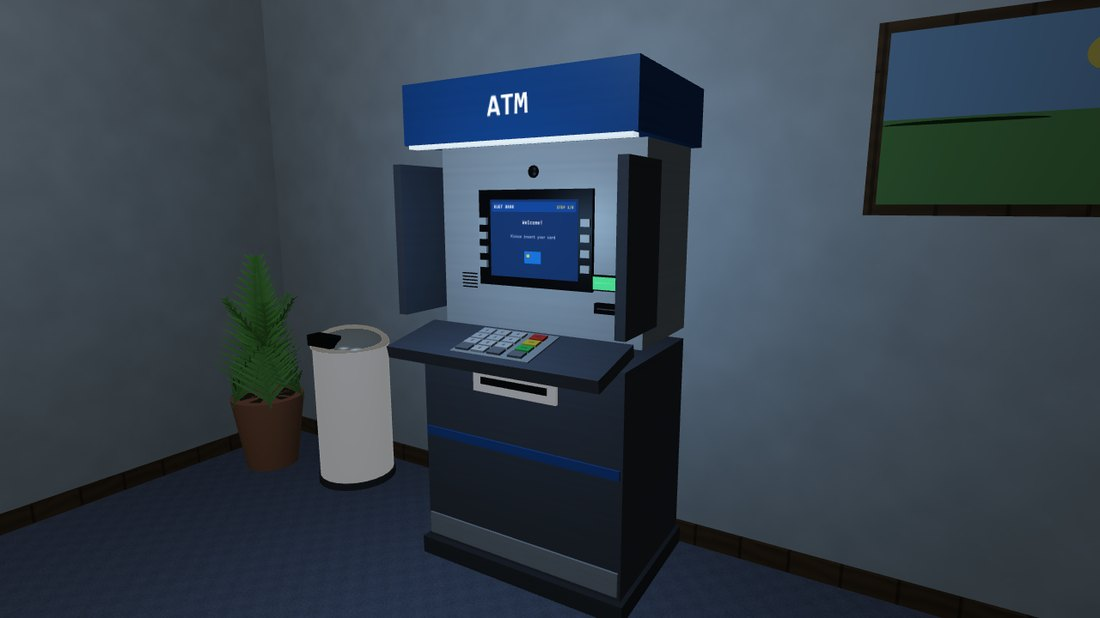
\includegraphics[width=\linewidth]{tour_atm}\caption{ATM room}\end{subfigure}
\begin{subfigure}{0.49\linewidth}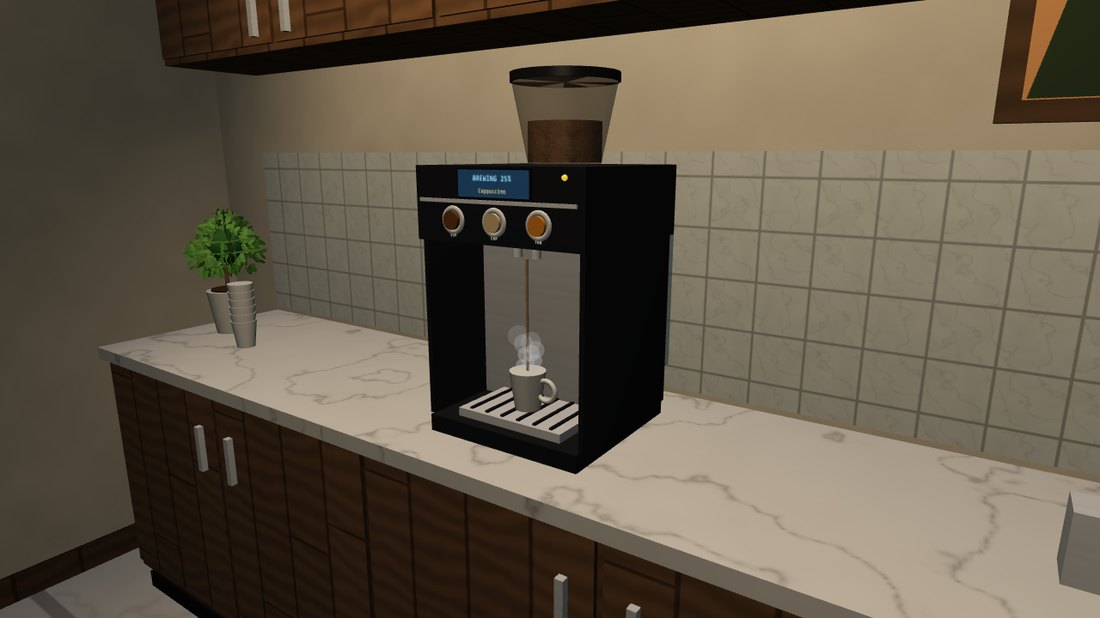
\includegraphics[width=\linewidth]{tour_coffee}\caption{Coffee machine (brewing)}\end{subfigure}
\begin{subfigure}{0.49\linewidth}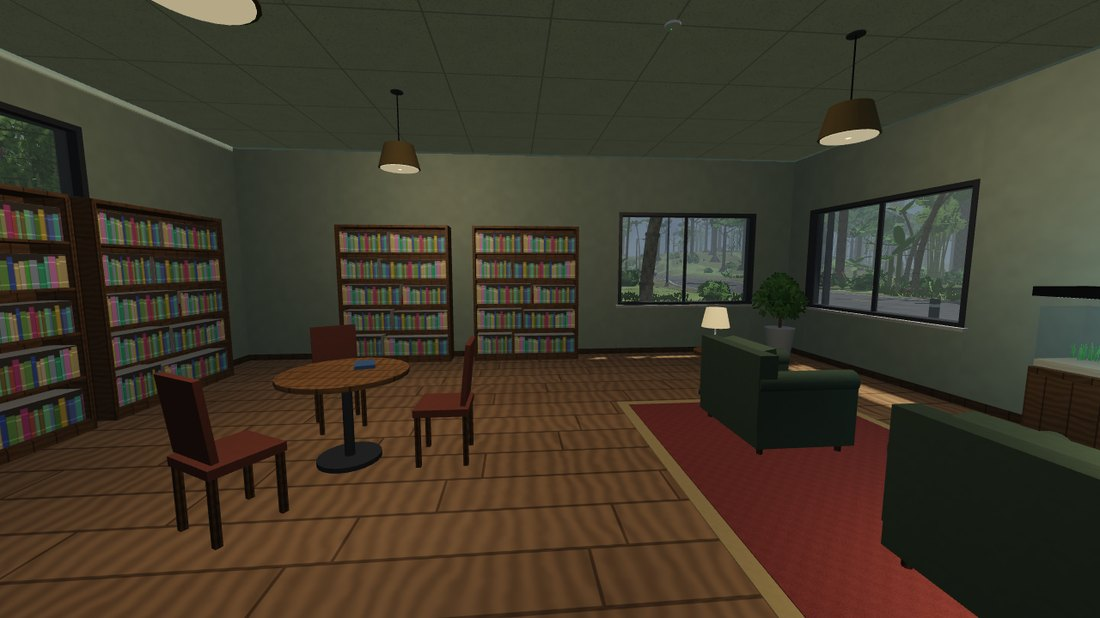
\includegraphics[width=\linewidth]{library_day}\caption{Library}\end{subfigure}
\begin{subfigure}{0.49\linewidth}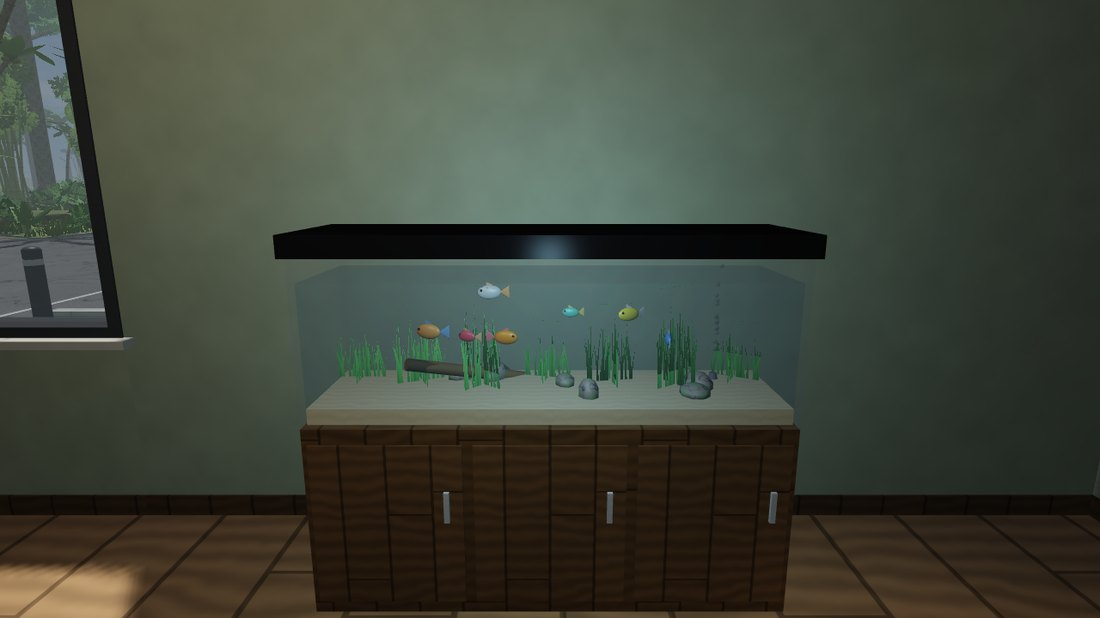
\includegraphics[width=\linewidth]{aquarium}\caption{Aquarium in the library}\end{subfigure}
\caption{The ATM room, the coffee counter and the library.}\label{fig:rooms}
\end{figure}
\begin{figure}[H]
\centering
\begin{subfigure}{0.49\linewidth}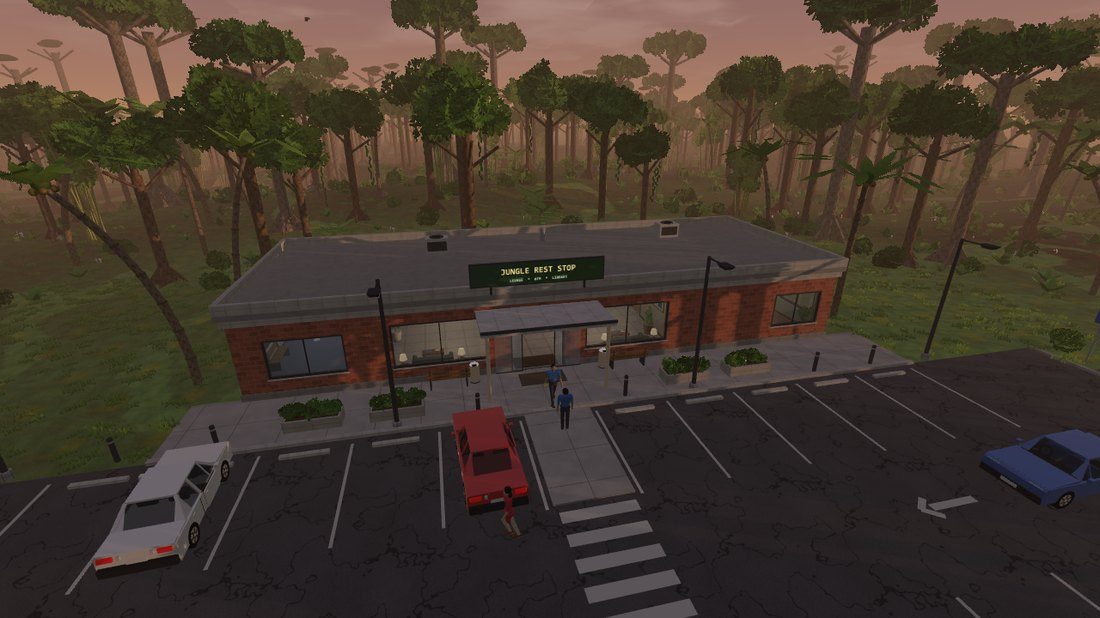
\includegraphics[width=\linewidth]{ext_sunrise}\caption{Sunrise 6:18}\end{subfigure}
\begin{subfigure}{0.49\linewidth}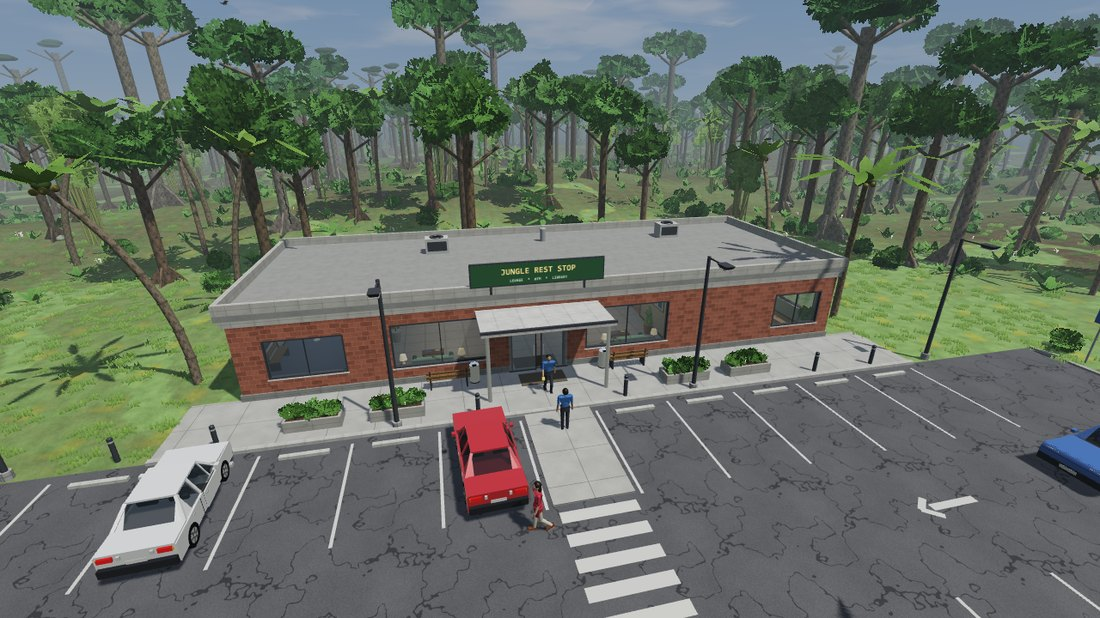
\includegraphics[width=\linewidth]{ext_day}\caption{Day 10:30}\end{subfigure}
\begin{subfigure}{0.49\linewidth}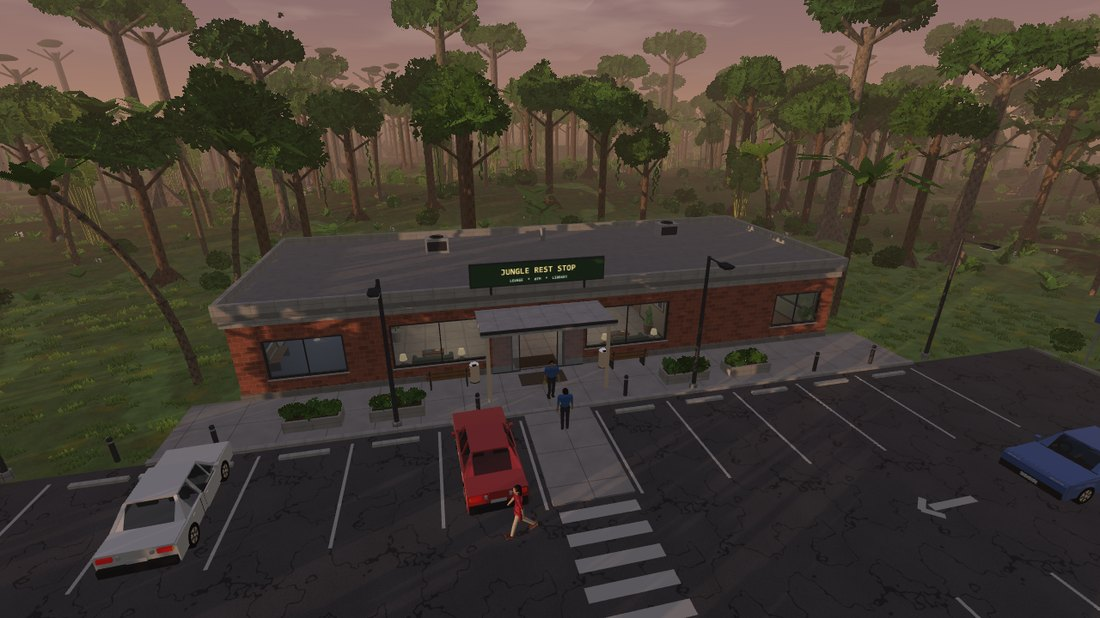
\includegraphics[width=\linewidth]{ext_sunset}\caption{Sunset 17:36}\end{subfigure}
\begin{subfigure}{0.49\linewidth}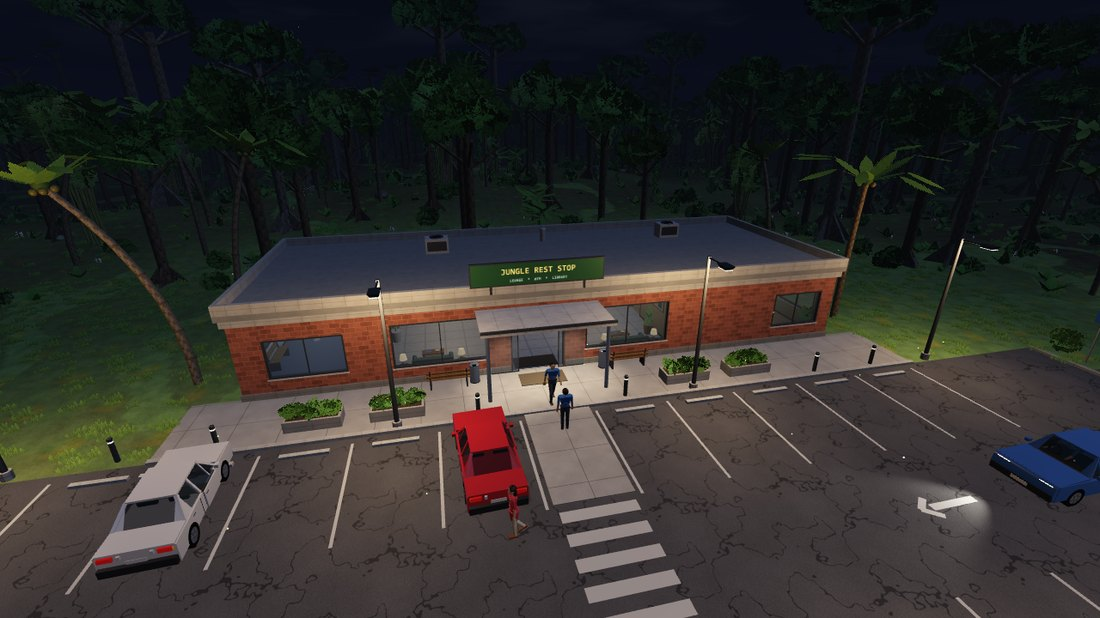
\includegraphics[width=\linewidth]{ext_night}\caption{Night 21:00}\end{subfigure}
\caption{The same view at four times of day.}\label{fig:daytimes}
\end{figure}

% =============================================================================
\section{Tools and Environment}
\begin{table}[H]
\centering\small
\begin{tabular}{@{}ll@{}}
\toprule
Item & Used \\ \midrule
Language & C++17 (MinGW-w64 / MSYS2 \texttt{g++}) \\
Graphics API & OpenGL 3.3 Core profile, GLSL 330 \\
Window / input & GLFW 3 \\
OpenGL loader & GLAD 2 \\
Text & Windows GDI renders one font atlas at start-up (Consolas) \\
Sound & Windows \texttt{waveOut} (winmm); 14 short CC0 (public domain) recordings \\
Assets & no models, no images: all meshes and textures are generated in code; only the sounds are files \\
Test PC & Intel Core i5-1135G7, Intel Iris Xe (integrated GPU), 1280$\times$720 window, 4$\times$MSAA \\
\bottomrule
\end{tabular}
\end{table}

% =============================================================================
\section{Controls}\label{sec:controls}
The scene is controlled with the keyboard and the mouse. Pressing \textbf{H} shows the same list inside
the program (\Cref{fig:help}).
\begin{table}[H]
\centering\small
\caption{Keyboard and mouse controls}\label{tab:controls}
\begin{tabularx}{\linewidth}{@{}P{3.3cm}X P{3.0cm}X@{}}
\toprule
Key & Action & Key & Action \\ \midrule
W A S D & walk & Shift & run \\
Mouse & look around & Space & jump \\
E / left click & use the part under the crosshair & V & camera: first person, third person, free \\
Mouse wheel, + / -- & change the field of view & Alt & free the mouse to click the on-screen buttons \\
B & Basic / Enhanced rendering & T, G, F & textures, shadows, fog on / off \\
N & switch day / night & [ \ ] & slower / faster time \\
M & pause the clock & R & roof cut-away view \\
F1 -- F4 & lounge, spot, room and outdoor lights & K & call a visitor car \\
L & frame cap 30 / 60 FPS & O & sound on / off \\
F12 & save a screenshot & H, Esc & help screen, quit \\
\bottomrule
\end{tabularx}
\end{table}
\begin{figure}[H]\centering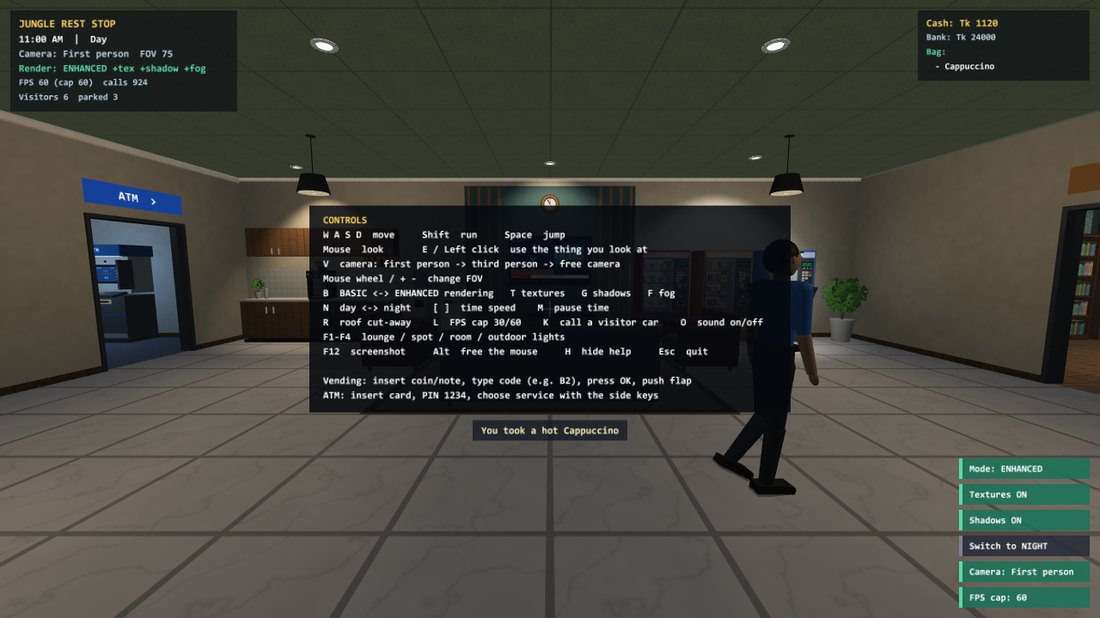
\includegraphics[width=0.8\linewidth]{help_screen}\caption{The help screen (H), with the status panel (top left), the wallet and the bag (top right) and the clickable buttons (bottom right).}\label{fig:help}\end{figure}

% =============================================================================
\section{System Design}
\subsection{Modules}
The code is divided into small modules, each with a single responsibility (\Cref{fig:modules}).

\begin{figure}[H]
\centering
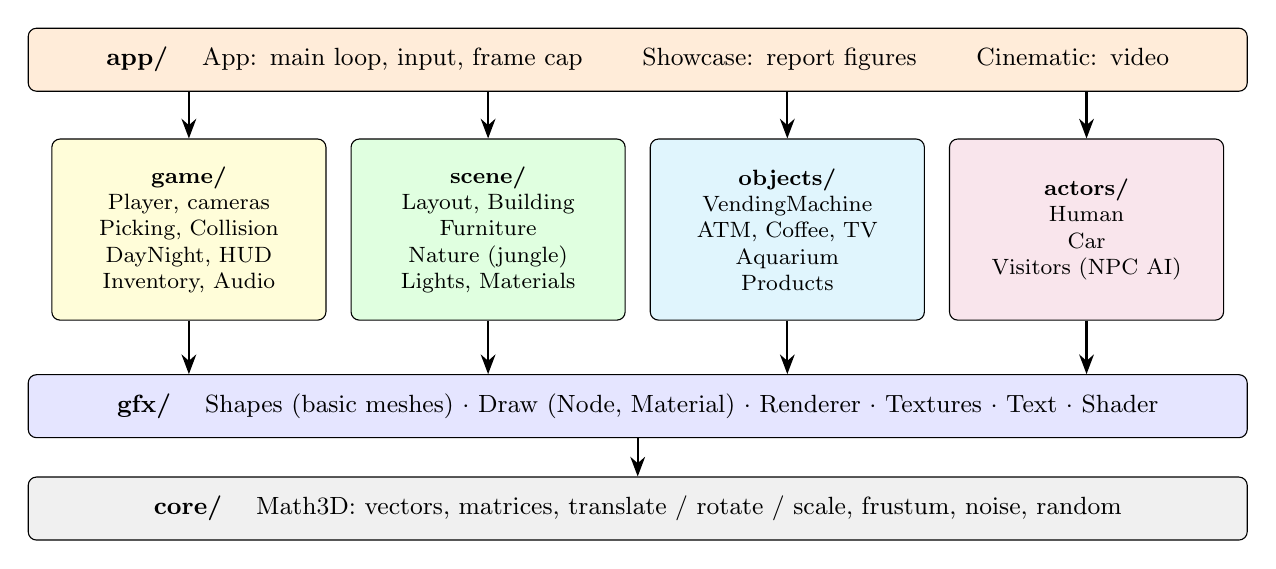
\begin{tikzpicture}[mod/.style={draw,rounded corners=3pt,align=center,font=\footnotesize,inner sep=4pt,text width=3.2cm,minimum height=2.3cm,anchor=north},
  wide/.style={draw,rounded corners=3pt,align=center,font=\small,inner sep=4pt,text width=15.2cm,minimum height=0.8cm}]
\node[wide,fill=orange!15] (app) at (0,0) {\textbf{app/} \quad App: main loop, input, frame cap \qquad Showcase: report figures \qquad Cinematic: video};
\node[mod,fill=yellow!15] (game) at (-5.7,-1.0) {\textbf{game/}\\Player, cameras\\Picking, Collision\\DayNight, HUD\\Inventory, Audio};
\node[mod,fill=green!12] (scene) at (-1.9,-1.0) {\textbf{scene/}\\Layout, Building\\Furniture\\Nature (jungle)\\Lights, Materials};
\node[mod,fill=cyan!12] (objects) at (1.9,-1.0) {\textbf{objects/}\\VendingMachine\\ATM, Coffee, TV\\Aquarium\\Products};
\node[mod,fill=purple!10] (actors) at (5.7,-1.0) {\textbf{actors/}\\Human\\Car\\Visitors (NPC AI)};
\node[wide,fill=blue!10] (gfx) at (0,-4.4) {\textbf{gfx/} \quad Shapes (basic meshes) $\cdot$ Draw (Node, Material) $\cdot$ Renderer $\cdot$ Textures $\cdot$ Text $\cdot$ Shader};
\node[wide,fill=gray!12] (core) at (0,-5.7) {\textbf{core/} \quad Math3D: vectors, matrices, translate / rotate / scale, frustum, noise, random};
\foreach \n in {game,scene,objects,actors} {
  \draw[arr] (\n.north |- app.south) -- (\n.north);
  \draw[arr] (\n.south) -- (\n.south |- gfx.north);
}
\draw[arr] (gfx) -- (core);
\end{tikzpicture}
\caption{Module overview. Arrows mean ``uses''.}\label{fig:modules}
\end{figure}

\subsection{Frame loop}
Each frame runs the same sequence (\Cref{fig:loop}). All movement uses the measured frame time
$\Delta t$, so every animation has the same speed at 30 and at 60 frames per second.
\begin{figure}[H]
\centering
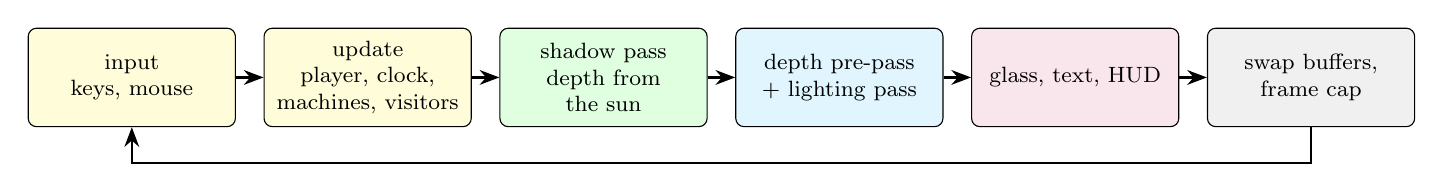
\begin{tikzpicture}[node distance=0.35cm,b/.style={box,text width=2.35cm,minimum height=1.25cm,font=\footnotesize}]
\node[b,fill=yellow!15] (in) {input\\keys, mouse};
\node[b,fill=yellow!15,right=of in] (up) {update\\player, clock, machines, visitors};
\node[b,fill=green!12,right=of up] (sh) {shadow pass\\depth from the sun};
\node[b,fill=cyan!12,right=of sh] (op) {depth pre-pass + lighting pass};
\node[b,fill=purple!10,right=of op] (tr) {glass, text, HUD};
\node[b,fill=gray!12,right=of tr] (cap) {swap buffers, frame cap};
\draw[arr] (in)--(up); \draw[arr] (up)--(sh); \draw[arr] (sh)--(op); \draw[arr] (op)--(tr); \draw[arr] (tr)--(cap);
\draw[arr] (cap.south) -- ++(0,-0.45) -| (in.south);
\end{tikzpicture}
\caption{One frame of the program.}\label{fig:loop}
\end{figure}

\subsection{Scene layout}
\begin{figure}[H]
\centering
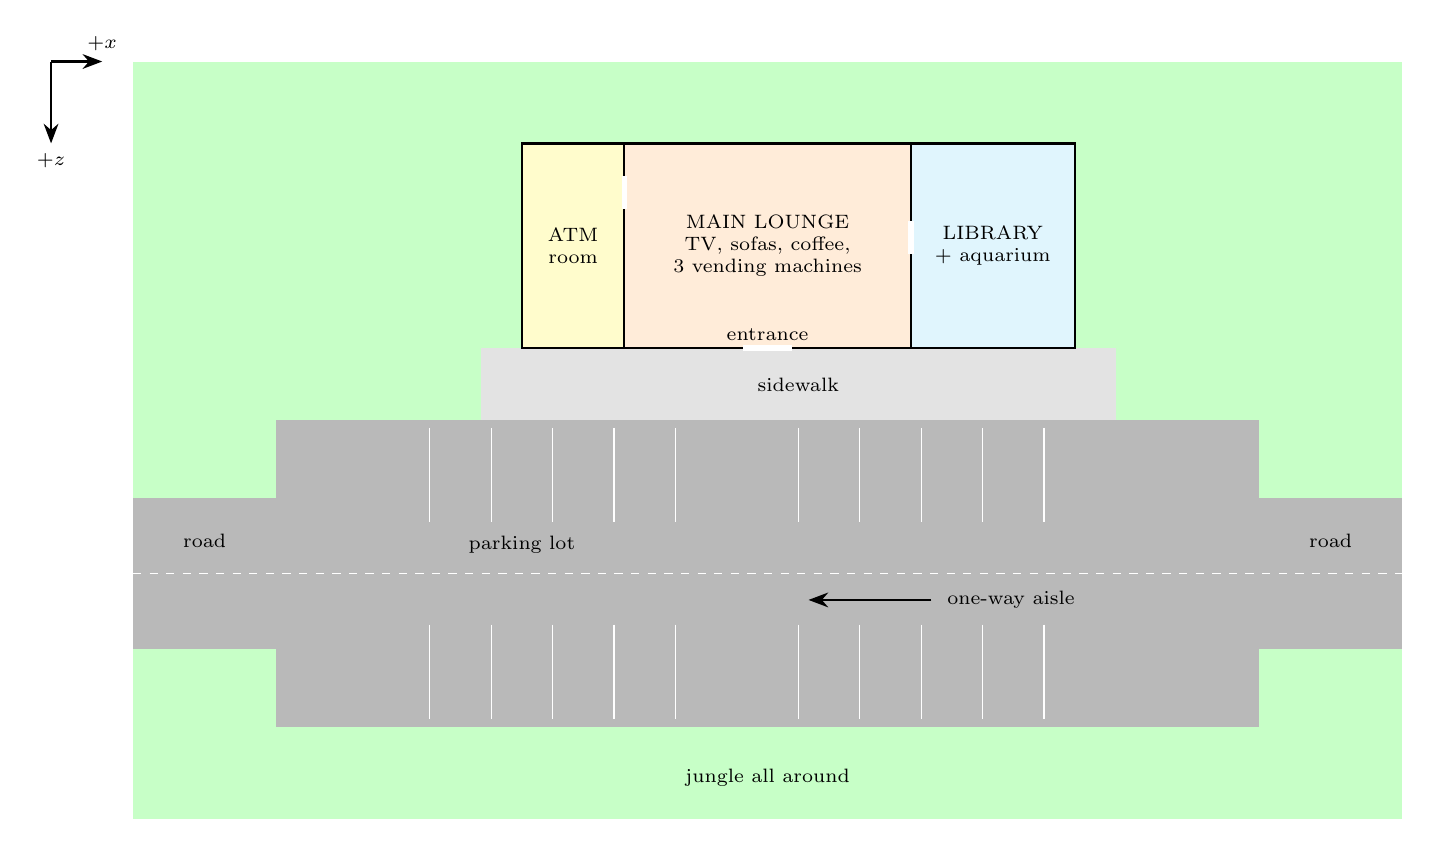
\begin{tikzpicture}[x=0.26cm,y=-0.26cm,lab/.style={font=\scriptsize,align=center}]
\fill[green!22!white] (-31,-9) rectangle (31,28);
\fill[gray!55] (-24,8.5) rectangle (24,23.5);
\fill[gray!55] (-31,12.3) rectangle (-24,19.7); \fill[gray!55] (24,12.3) rectangle (31,19.7);
\fill[gray!22] (-14,5) rectangle (17,8.5);
\draw[thick,fill=yellow!20] (-12,-5) rectangle (-7,5);
\draw[thick,fill=orange!15] (-7,-5) rectangle (7,5);
\draw[thick,fill=cyan!12] (7,-5) rectangle (15,5);
\node[lab] at (-9.5,0) {ATM\\room};
\node[lab] at (0,0) {MAIN LOUNGE\\TV, sofas, coffee,\\3 vending machines};
\node[lab] at (11,0) {LIBRARY\\+ aquarium};
\draw[line width=2pt,white] (-1.2,5) -- (1.2,5);
\draw[line width=2pt,white] (-7,-3.4) -- (-7,-1.8);
\draw[line width=2pt,white] (7,-1.2) -- (7,0.4);
\node[lab,anchor=south] at (0,5.1) {entrance};
\foreach \i in {-15,-12,-9,-6,-3,3,6,9,12,15} {\draw[white] (\i-1.5,8.9)--(\i-1.5,13.5); \draw[white] (\i-1.5,18.5)--(\i-1.5,23.1);}
\draw[white,dashed] (-31,16) -- (31,16);
\node[lab] at (1.5,6.8) {sidewalk};
\node[lab] at (-12,14.6) {parking lot};
\node[lab] at (-27.5,14.4) {road};
\node[lab] at (27.5,14.4) {road};
\draw[arr] (8,17.3) -- (2,17.3); \node[lab,anchor=west] at (8.3,17.3) {one-way aisle};
\node[lab] at (0,26) {jungle all around};
\draw[arr] (-35,-9) -- (-35,-5) node[below,font=\scriptsize]{$+z$};
\draw[arr] (-35,-9) -- (-32.5,-9) node[above,font=\scriptsize]{$+x$};
\end{tikzpicture}
\caption{Top view of the layout (1 grid unit = 1 m). The building faces $+z$, towards the parking lot.}\label{fig:layout}
\end{figure}

% =============================================================================
\section{The Basic Shapes}\label{sec:shapes}
All objects are built from the fifteen \emph{unit} meshes listed in \Cref{tab:shapes}. Each mesh is
centred at the origin and has a size of about one unit, so a part of any size is obtained by scaling it.
The meshes are generated once at start-up (\texttt{gfx/Shapes.cpp}) and stay on the GPU; every part of
every object is only a reference to one of these meshes plus a $4\times4$ matrix. The pictures show each
mesh with the edges of its triangles drawn on top.

\paragraph{Generation rules.} Flat shapes are written as lists of corner points. Every face has its own
vertices, so that the face has one flat normal and the edges stay sharp; a quad face $(a,b,c,d)$ is split
into the triangles $(a,b,c)$ and $(a,c,d)$. Round shapes are generated by loops over angles. For a ring of
$n$ steps the angle is $\theta_i = 2\pi i/n$, and the side of a cylinder with bottom radius $r_b$ and top
radius $r_t$ uses
\[
\mathbf{p}_i^{top} = (r_t\cos\theta_i,\ 0.5,\ r_t\sin\theta_i),\quad
\mathbf{p}_i^{bot} = (r_b\cos\theta_i,\ -0.5,\ r_b\sin\theta_i),\quad
\mathbf{n}_i = \operatorname{normalize}(\cos\theta_i,\ r_b-r_t,\ \sin\theta_i).
\]
Neighbouring ring points form one side quad
$(\mathbf{p}_i^{bot},\ \mathbf{p}_{i+1}^{bot},\ \mathbf{p}_{i+1}^{top},\ \mathbf{p}_i^{top})$,
and a cap is a fan of triangles around the centre vertex $(0,\pm0.5,0)$. Round shapes have one normal per
vertex pointing straight out of the surface, so they look smooth even with few sides.

{\small
\setlength{\tabcolsep}{4pt}
\begin{longtable}{@{}c P{2.1cm} P{8.2cm} r@{}}
\caption{The basic shapes, how their vertices are generated, and their vertex / triangle counts}\label{tab:shapes}\\
\toprule
Shape & Name & Vertices & V / T \\ \midrule
\endfirsthead
\toprule
Shape & Name & Vertices & V / T \\ \midrule
\endhead
\bottomrule
\endfoot
\raisebox{-0.8\height}{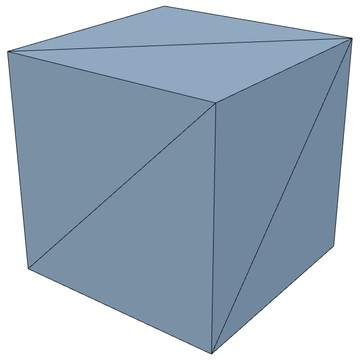
\includegraphics[width=2.1cm]{shape_0}} & Cube & 8 corners $(\pm.5,\pm.5,\pm.5)$ (\Cref{fig:cube}); each of the 6 faces has its own 4 vertices and the face normal & \svCube\ / \stCube \\
\raisebox{-0.8\height}{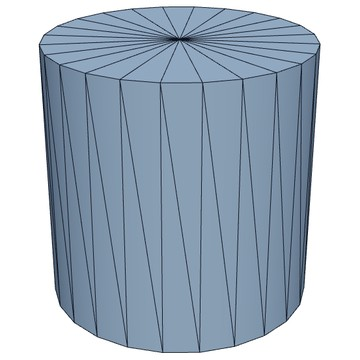
\includegraphics[width=2.1cm]{shape_1}} & Cylinder & ring loop with $r_b=r_t=0.5$, $n=24$, two caps & \svCylinder\ / \stCylinder \\
\raisebox{-0.8\height}{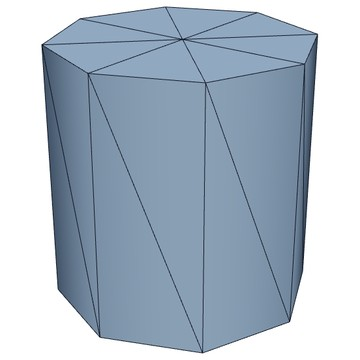
\includegraphics[width=2.1cm]{shape_2}} & Cylinder (low) & the same with $n=8$; used for tree trunks and bamboo & \svCylinderLow\ / \stCylinderLow \\
\raisebox{-0.8\height}{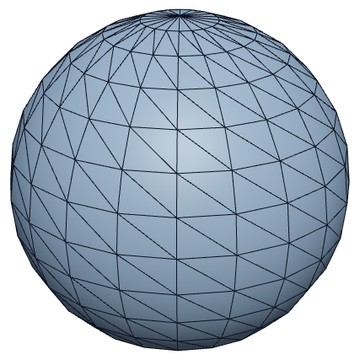
\includegraphics[width=2.1cm]{shape_3}} & Sphere & $\mathbf{p}_{ij}=0.5(\sin\phi_i\cos\theta_j,\ \cos\phi_i,\ \sin\phi_i\sin\theta_j)$, $\phi_i=\pi i/14$, $\theta_j=2\pi j/20$, normal $\mathbf{n}=2\mathbf{p}$ & \svSphere\ / \stSphere \\
\raisebox{-0.8\height}{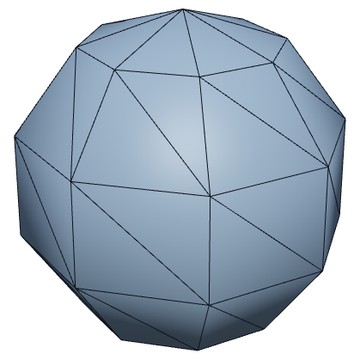
\includegraphics[width=2.1cm]{shape_4}} & Sphere (low) & the same with 5 rings and 8 sectors; foliage blobs, rocks & \svSphereLow\ / \stSphereLow \\
\raisebox{-0.8\height}{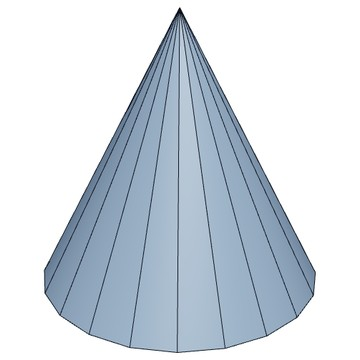
\includegraphics[width=2.1cm]{shape_5}} & Cone & ring loop with $r_t=0$ (all top vertices meet at the tip $(0,0.5,0)$), $n=20$, bottom cap & \svCone\ / \stCone \\
\raisebox{-0.8\height}{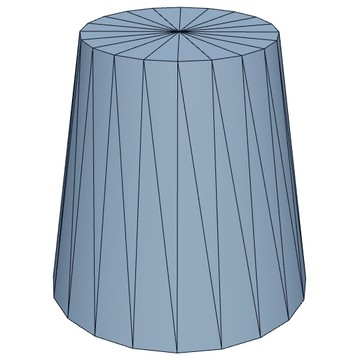
\includegraphics[width=2.1cm]{shape_6}} & Truncated cone & ring loop with $r_t=0.35$, $n=20$, two caps; cups, pots, limbs & \svTruncatedCone\ / \stTruncatedCone \\
\raisebox{-0.8\height}{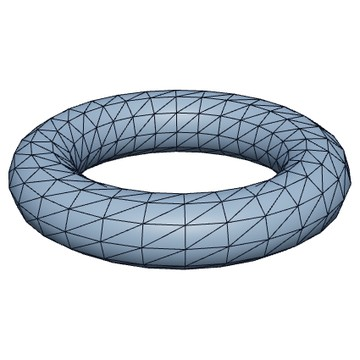
\includegraphics[width=2.1cm]{shape_7}} & Torus & $\mathbf{p}(u,w)=(0.4+0.1\cos w)(\cos u,0,\sin u)+(0,0.1\sin w,0)$, $28\times10$ steps & \svTorus\ / \stTorus \\
\raisebox{-0.8\height}{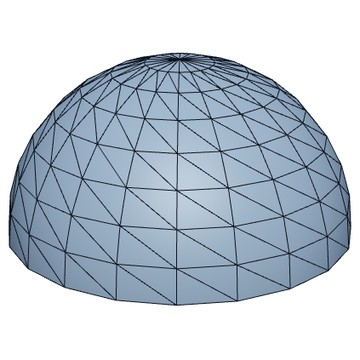
\includegraphics[width=2.1cm]{shape_8}} & Hemisphere & sphere formula with $\phi\in[0,\pi/2]$ (8 rings) plus a flat disc at $y=0$ & \svHemisphere\ / \stHemisphere \\
\raisebox{-0.8\height}{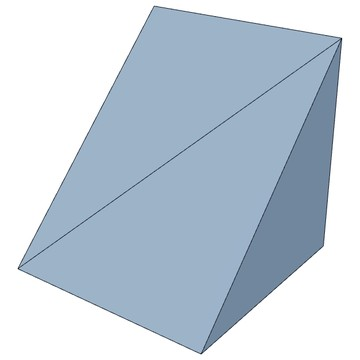
\includegraphics[width=2.1cm]{shape_9}} & Wedge & left side $w_0(-.5,-.5,.5)$, $w_1(-.5,-.5,-.5)$, $w_2(-.5,.5,-.5)$; right side $w_3,w_4,w_5$ = the same with $x=+.5$; 2 triangles and 3 quads & \svWedge\ / \stWedge \\
\raisebox{-0.8\height}{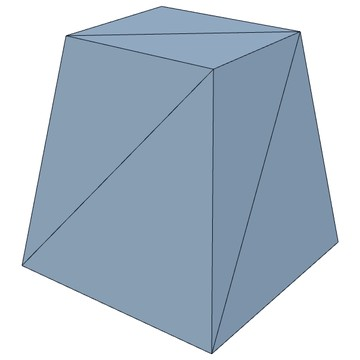
\includegraphics[width=2.1cm]{shape_10}} & Tapered box & bottom corners $(\pm.5,-.5,\pm.5)$, top corners $(\pm.35,.5,\pm.3)$; side normal $\mathbf{n}=\operatorname{normalize}((\mathbf{b}-\mathbf{a})\times(\mathbf{d}-\mathbf{a}))$ & \svTaperedBox\ / \stTaperedBox \\
\raisebox{-0.8\height}{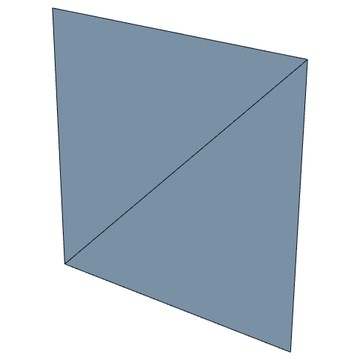
\includegraphics[width=2.1cm]{shape_11}} & Quad & $(-.5,-.5,0)$, $(.5,-.5,0)$, $(.5,.5,0)$, $(-.5,.5,0)$, normal $(0,0,1)$; fronds, vines & \svQuad\ / \stQuad \\
\raisebox{-0.8\height}{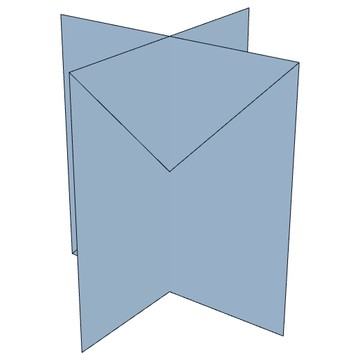
\includegraphics[width=2.1cm]{shape_12}} & Cross card & two crossed quads with $y\in[0,1]$ (base on the ground); grass, ferns, flowers & \svCrossCard\ / \stCrossCard \\
\raisebox{-0.8\height}{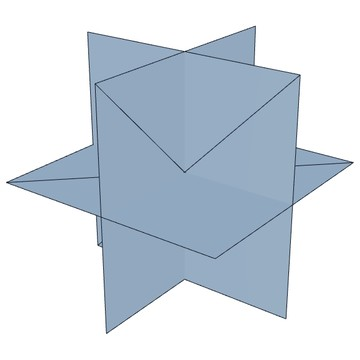
\includegraphics[width=2.1cm]{shape_13}} & Leaf card & three quads through the centre, one in each plane ($xy$, $yz$, $xz$); leaf clusters & \svLeafCard\ / \stLeafCard \\
\raisebox{-0.8\height}{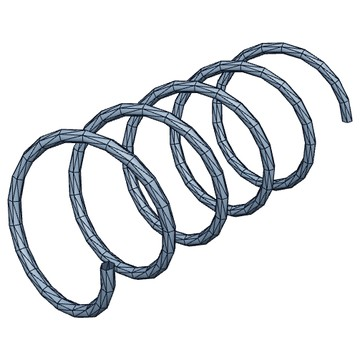
\includegraphics[width=2.1cm]{shape_14}} & Coil & a 6-sided ring around each of 101 points of the helix $\mathbf{c}(t)=(R\cos 2\pi kt,\ R\sin 2\pi kt,\ L(t-0.5))$, $k=5$ turns & \svCoil\ / \stCoil \\
\end{longtable}}

\begin{figure}[H]
\centering
\begin{minipage}{0.40\linewidth}
\centering
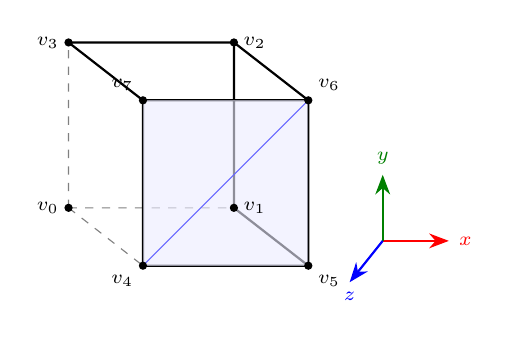
\begin{tikzpicture}[scale=2.1,font=\scriptsize]
\coordinate (v0) at (0,0); \coordinate (v1) at (1,0); \coordinate (v2) at (1,1); \coordinate (v3) at (0,1);
\coordinate (v4) at (0.45,-0.35); \coordinate (v5) at (1.45,-0.35); \coordinate (v6) at (1.45,0.65); \coordinate (v7) at (0.45,0.65);
\draw[dashed,gray] (v0)--(v1) (v0)--(v3) (v0)--(v4);
\draw[thick] (v1)--(v2)--(v3) (v4)--(v5)--(v6)--(v7)--cycle (v1)--(v5) (v2)--(v6) (v3)--(v7);
\fill[blue!8,opacity=0.6] (v4)--(v5)--(v6)--(v7)--cycle;
\draw[blue!60] (v4)--(v6);
\foreach \i/\p in {0/left,1/right,2/right,3/left,4/below left,5/below right,6/above right,7/above left} \fill (v\i) circle (0.025) node[\p] {$v_\i$};
\draw[arr,red] (1.9,-0.2)--(2.3,-0.2) node[right]{$x$};
\draw[arr,green!50!black] (1.9,-0.2)--(1.9,0.2) node[above]{$y$};
\draw[arr,blue] (1.9,-0.2)--(1.7,-0.45) node[below]{$z$};
\end{tikzpicture}
\end{minipage}\hfill
\begin{minipage}{0.56\linewidth}
\centering\small
\begin{tabular}{@{}cc|cc@{}}
\toprule
Corner & $(x,y,z)$ & Corner & $(x,y,z)$ \\ \midrule
$v_0$ & $(-.5,-.5,-.5)$ & $v_4$ & $(-.5,-.5,\ .5)$ \\
$v_1$ & $(\ .5,-.5,-.5)$ & $v_5$ & $(\ .5,-.5,\ .5)$ \\
$v_2$ & $(\ .5,\ .5,-.5)$ & $v_6$ & $(\ .5,\ .5,\ .5)$ \\
$v_3$ & $(-.5,\ .5,-.5)$ & $v_7$ & $(-.5,\ .5,\ .5)$ \\
\bottomrule
\end{tabular}

\vspace{0.5em}
Faces: front $(v_4v_5v_6v_7)$, back $(v_1v_0v_3v_2)$, top $(v_7v_6v_2v_3)$,
bottom $(v_0v_1v_5v_4)$, right $(v_5v_1v_2v_6)$, left $(v_0v_4v_7v_3)$.
The front face is split into $(v_4v_5v_6)$ and $(v_4v_6v_7)$.
\end{minipage}
\caption{The unit cube: 8 corners, 6 faces, 12 triangles. The front face (shaded) looks towards $+z$.}\label{fig:cube}
\end{figure}

The ground is one more generated mesh: a $150\times150$ grid whose vertices are lifted to the terrain
height $h(x,z)$ (\Cref{sec:terrain}).

% =============================================================================
\section{Transformations and Hierarchical Modelling}\label{sec:transform}
\subsection{Homogeneous coordinates and the basic transformations}
A point is written as $\mathbf{p}=(x,y,z,1)^T$, so that translation, rotation and scaling are all
$4\times4$ matrix products. The matrices are stored column-major and sent to OpenGL unchanged.
\[
T(\mathbf{t})=\begin{bmatrix}1&0&0&t_x\\0&1&0&t_y\\0&0&1&t_z\\0&0&0&1\end{bmatrix}\qquad
S(\mathbf{s})=\begin{bmatrix}s_x&0&0&0\\0&s_y&0&0\\0&0&s_z&0\\0&0&0&1\end{bmatrix}
\]
\[
R_x(\theta)=\begin{bmatrix}1&0&0&0\\0&\cos\theta&-\sin\theta&0\\0&\sin\theta&\cos\theta&0\\0&0&0&1\end{bmatrix}\quad
R_y(\theta)=\begin{bmatrix}\cos\theta&0&\sin\theta&0\\0&1&0&0\\-\sin\theta&0&\cos\theta&0\\0&0&0&1\end{bmatrix}\quad
R_z(\theta)=\begin{bmatrix}\cos\theta&-\sin\theta&0&0\\\sin\theta&\cos\theta&0&0\\0&0&1&0\\0&0&0&1\end{bmatrix}
\]
A rotation given in degrees $(\theta_x,\theta_y,\theta_z)$ is applied as $R=R_y(\theta_y)\,R_x(\theta_x)\,R_z(\theta_z)$.
Rotation about an arbitrary unit axis $\mathbf{a}$ uses Rodrigues' formula
\[
R(\mathbf{a},\theta) = \cos\theta\,I + (1-\cos\theta)\,\mathbf{a}\mathbf{a}^T + \sin\theta\,[\mathbf{a}]_\times,\qquad
[\mathbf{a}]_\times=\begin{bmatrix}0&-a_z&a_y\\a_z&0&-a_x\\-a_y&a_x&0\end{bmatrix}.
\]
A negative scale factor mirrors a part (used for the fruit bowl and for mirrored book rows).

\subsection{Composite transformation of a part}
Every part of every object is placed with
\[
M_{part} = M_{parent}\cdot T(\text{position})\cdot R(\text{rotation})\cdot S(\text{size}),\qquad
\mathbf{p}_{world} = M_{part}\,\mathbf{p}_{unit}.
\]
Read from right to left, the unit shape is first \textbf{scaled} to its size, then \textbf{rotated}, then
\textbf{translated} to its place inside the parent, and finally carried into the world by the parent's
matrix. The order matters: scaling after a rotation would shear the shape. Normals are transformed with
the normal matrix
\[
N = \big(M_{3\times3}^{-1}\big)^T,\qquad \mathbf{n}_{world} = \operatorname{normalize}(N\,\mathbf{n}),
\]
which keeps them perpendicular to the surface even when a shape is stretched unevenly.

\subsection{Hierarchical modelling with nodes}
Objects are written as trees of \texttt{Node}s. A node stores the matrix of its coordinate frame; a child
node is created with an extra translation and rotation relative to its parent, so moving or turning a
parent moves all of its children:
\begin{lstlisting}
struct Node {
    DrawSink* sink;  Mat4 M;                          // M = this node's world matrix
    Node at(const Vec3& p, const Vec3& rotDeg) const  // child: M * T(p) * R(rot)
        { return Node(*sink, rotateYXZ(translate(M, p), rotDeg)); }
    void part(MeshId mesh, Vec3 pos, Vec3 size, const Material& m, Vec3 rotDeg = {}) const
        { sink->add(mesh, scale(rotateYXZ(translate(M, pos), rotDeg), size), m); }
};
// a sofa arm: a box and a cylinder lying along z (rotated 90 degrees about x)
n.box({x, 0.42f, 0.0f}, {0.16f, 0.44f, 0.88f}, fabric);
n.part(M_CYLINDER, {x, 0.64f, 0.0f}, {0.19f, 0.88f, 0.19f}, fabric, {90, 0, 0});
\end{lstlisting}
The same object code can send its shapes to different \emph{sinks}: the static world, the per-frame list,
a counter, or a collector that records every part with its name (used for the exploded views and part
tables in \Cref{sec:objects}).

\paragraph{A matrix built from corner points.} Some parts are not rectangles (car windows, door glass).
For a parallelogram with corners $\mathbf{a}$, $\mathbf{b}$, $\mathbf{d}$ and $\mathbf{b}+\mathbf{d}-\mathbf{a}$
the model matrix is built directly from the edge vectors:
\[
M = \begin{bmatrix} \mathbf{b}-\mathbf{a} & \mathbf{d}-\mathbf{a} & t\,\hat{\mathbf{n}} & \mathbf{a}+\tfrac12(\mathbf{b}-\mathbf{a})+\tfrac12(\mathbf{d}-\mathbf{a}) \\ 0&0&0&1\end{bmatrix},
\qquad \hat{\mathbf{n}}=\frac{(\mathbf{b}-\mathbf{a})\times(\mathbf{d}-\mathbf{a})}{|(\mathbf{b}-\mathbf{a})\times(\mathbf{d}-\mathbf{a})|},
\]
where $t$ is the thickness. The unit cube corner $(-.5,-.5,0)$ lands exactly on $\mathbf{a}$, $(.5,-.5,0)$
on $\mathbf{b}$ and $(-.5,.5,0)$ on $\mathbf{d}$. A triangle is made the same way from the wedge.
A \emph{beam} between two points $\mathbf{a}$ and $\mathbf{b}$ (pillars, branches) turns the shape's $y$ axis
onto $\mathbf{d}=\mathbf{b}-\mathbf{a}$ with the axis $\mathbf{y}\times\hat{\mathbf{d}}$ and the angle
$\operatorname{atan2}(|\mathbf{y}\times\hat{\mathbf{d}}|,\ \mathbf{y}\cdot\hat{\mathbf{d}})$, and scales it to
the length $|\mathbf{d}|$.

\subsection{Viewing and projection}
The camera matrix is built with \texttt{lookAt} from the eye $\mathbf{e}$, the target $\mathbf{c}$ and the up
vector $\mathbf{u}$:
\[
\mathbf{f}=\frac{\mathbf{c}-\mathbf{e}}{|\mathbf{c}-\mathbf{e}|},\quad
\mathbf{s}=\frac{\mathbf{f}\times\mathbf{u}}{|\mathbf{f}\times\mathbf{u}|},\quad
\mathbf{u}'=\mathbf{s}\times\mathbf{f},\qquad
V=\begin{bmatrix} s_x&s_y&s_z&-\mathbf{s}\cdot\mathbf{e}\\ u'_x&u'_y&u'_z&-\mathbf{u}'\cdot\mathbf{e}\\ -f_x&-f_y&-f_z&\mathbf{f}\cdot\mathbf{e}\\0&0&0&1\end{bmatrix}.
\]
The main view uses a perspective projection with vertical field of view $f$, aspect ratio $a$ and the
near and far planes $z_n$, $z_f$. The sun's shadow camera and the 2D text overlay use orthographic
projections:
\[
P_{persp} = \begin{bmatrix}\frac{1}{a\tan(f/2)}&0&0&0\\0&\frac{1}{\tan(f/2)}&0&0\\0&0&-\frac{z_f+z_n}{z_f-z_n}&-\frac{2z_fz_n}{z_f-z_n}\\0&0&-1&0\end{bmatrix}
\qquad
P_{ortho} = \begin{bmatrix}\frac{2}{r-l}&0&0&-\frac{r+l}{r-l}\\0&\frac{2}{t-b}&0&-\frac{t+b}{t-b}\\0&0&\frac{-2}{z_f-z_n}&-\frac{z_f+z_n}{z_f-z_n}\\0&0&0&1\end{bmatrix}.
\]
A vertex therefore goes through $\mathbf{p}_{clip}=P\,V\,M\,\mathbf{p}$, the perspective division
$\mathbf{p}_{ndc}=\mathbf{p}_{clip}/w_{clip}$, and the viewport transformation to pixels,
\[
x_{win} = \tfrac{W}{2}\,(x_{ndc}+1),\qquad y_{win}=\tfrac{H}{2}\,(y_{ndc}+1),\qquad z_{win}=\tfrac12(z_{ndc}+1).
\]
The field of view $f$ is changed with the mouse wheel between $25^\circ$ and $110^\circ$ (\Cref{sec:camera}),
and the aspect ratio $a=W/H$ follows the window size when the window is resized.

% =============================================================================
\section{The Objects}\label{sec:objects}
Each object is shown complete and with its parts pulled apart, followed by the basic shapes it uses
and the transformation of every part. For the main objects, the world coordinates of their key parts are
also listed. All tables are produced by the program from the drawing code of the scene.
\Cref{tab:parts} summarises the number of basic shapes of each object.
The world-coordinate tables give, for each key part, two vertices A and B that really exist in the mesh of its
shape (\Cref{tab:vertexpair}); their world position is $\mathbf{p}_{world}=M_{place}\,M_{part}\,\mathbf{v}$.
\begin{table}[H]
\centering\small
\caption{The two mesh vertices A and B listed for each shape (unit-shape coordinates, \Cref{tab:shapes})}\label{tab:vertexpair}
\begin{tabular}{@{}l l l l@{}}
\toprule
Shape & Vertex A & Vertex B & Which vertices \\ \midrule
cube & $(-.5,-.5,-.5)$ & $(.5,.5,.5)$ & opposite corners $v_0$ and $v_6$ (\Cref{fig:cube}) \\
cylinder & $(.5,-.5,0)$ & $(.5,.5,0)$ & first vertex of the bottom ring and of the top ring ($\theta_0=0$) \\
truncated cone & $(.5,-.5,0)$ & $(.35,.5,0)$ & first vertex of the bottom ring and of the top ring \\
cone & $(.5,-.5,0)$ & $(0,.5,0)$ & first vertex of the bottom ring, and the tip \\
sphere & $(0,-.5,0)$ & $(0,.5,0)$ & the two poles ($\phi=\pi$ and $\phi=0$) \\
hemisphere & $(.5,0,0)$ & $(0,.5,0)$ & first vertex of the rim, and the pole \\
torus & $(.5,0,0)$ & $(.3,0,0)$ & outer and inner edge of the tube at $u=0$ \\
wedge & $(-.5,-.5,.5)$ & $(.5,.5,-.5)$ & corners $w_0$ and $w_5$ \\
tapered box & $(-.5,-.5,-.5)$ & $(.35,.5,.3)$ & a bottom corner and a top corner \\
\bottomrule
\end{tabular}
\end{table}


\begin{table}[H]
\centering\scriptsize
\caption{Number of basic shapes per object (Cyl-L / Sph-L = low-poly versions, TCone = truncated cone, TBox = tapered box)}\label{tab:parts}
\setlength{\tabcolsep}{3.0pt}
\begin{tabular}{l r rrrrrrrrrrrrrrr}
\toprule
Object & Total & Cube & Cyl & Cyl-L & Sph & Sph-L & Cone & TCone & Torus & Hemi & Wedge & TBox & Quad & Cross & Leaf & Coil \\
\midrule
Vending machine & \textbf{287} & 79 & 177 & -- & 3 & -- & -- & 16 & -- & -- & -- & -- & -- & -- & -- & 12 \\
ATM & \textbf{49} & 48 & -- & -- & -- & -- & -- & -- & -- & 1 & -- & -- & -- & -- & -- & -- \\
Coffee machine & \textbf{32} & 16 & 9 & -- & 1 & -- & -- & 2 & 4 & -- & -- & -- & -- & -- & -- & -- \\
Television (frame) & \textbf{5} & 4 & -- & -- & 1 & -- & -- & -- & -- & -- & -- & -- & -- & -- & -- & -- \\
Sofa (3 seats) & \textbf{21} & 12 & 9 & -- & -- & -- & -- & -- & -- & -- & -- & -- & -- & -- & -- & -- \\
Armchair & \textbf{13} & 6 & 7 & -- & -- & -- & -- & -- & -- & -- & -- & -- & -- & -- & -- & -- \\
Bookshelf & \textbf{21} & 21 & -- & -- & -- & -- & -- & -- & -- & -- & -- & -- & -- & -- & -- & -- \\
Person (standing) & \textbf{41} & 9 & 11 & -- & 17 & -- & -- & 1 & 1 & 1 & -- & 1 & -- & -- & -- & -- \\
Person (walking) & \textbf{40} & 9 & 11 & -- & 17 & -- & -- & -- & 1 & 1 & -- & 1 & -- & -- & -- & -- \\
Person + chair & \textbf{47} & 15 & 11 & -- & 18 & -- & -- & -- & 1 & 1 & -- & 1 & -- & -- & -- & -- \\
Sedan car + driver & \textbf{115} & 63 & 28 & -- & 18 & -- & -- & -- & 2 & 1 & 1 & 2 & -- & -- & -- & -- \\
SUV + driver & \textbf{117} & 66 & 28 & -- & 18 & -- & -- & -- & 2 & 1 & 1 & 1 & -- & -- & -- & -- \\
Hatchback + driver & \textbf{114} & 62 & 28 & -- & 18 & -- & -- & -- & 2 & 1 & 1 & 2 & -- & -- & -- & -- \\
Rainforest tree & \textbf{27} & -- & -- & 5 & -- & 6 & -- & -- & -- & -- & 4 & -- & -- & -- & 12 & -- \\
Coconut palm & \textbf{37} & -- & -- & 14 & -- & 5 & -- & -- & -- & -- & -- & -- & 18 & -- & -- & -- \\
Bamboo clump & \textbf{130} & -- & -- & 100 & -- & -- & -- & -- & -- & -- & -- & -- & -- & -- & 30 & -- \\
Banana plant & \textbf{28} & -- & -- & 6 & -- & 22 & -- & -- & -- & -- & -- & -- & -- & -- & -- & -- \\
Street lamp & \textbf{5} & 1 & 2 & -- & -- & -- & -- & 1 & -- & -- & -- & 1 & -- & -- & -- & -- \\
Pendant lamp & \textbf{5} & -- & 3 & -- & 1 & -- & -- & 1 & -- & -- & -- & -- & -- & -- & -- & -- \\
Aquarium & \textbf{76} & 12 & -- & 1 & 35 & 6 & 7 & 1 & -- & -- & 7 & -- & -- & 7 & -- & -- \\
6 products & \textbf{23} & 9 & 12 & -- & 1 & -- & -- & 1 & -- & -- & -- & -- & -- & -- & -- & -- \\
Table set & \textbf{23} & 10 & 2 & -- & 3 & 1 & -- & 1 & -- & 1 & -- & -- & -- & -- & 5 & -- \\
Wall clock & \textbf{17} & 14 & 2 & -- & -- & -- & -- & -- & 1 & -- & -- & -- & -- & -- & -- & -- \\
Bush+fern+rock+log & \textbf{23} & -- & -- & 4 & -- & 8 & -- & -- & -- & 3 & -- & -- & 5 & 1 & 2 & -- \\
\bottomrule
\end{tabular}

\end{table}

% =============================================================================
\subsection{Machines}
% -----------------------------------------------------------------------------
\subsubsection{Vending machine}
The vending machine is $1.0\times1.95\times0.8$ m. Its origin is on the floor in the middle and it faces
$+z$. Three machines stand in the lounge: cold drinks (red), crispy snacks (orange) and sweet treats (blue).
\objviews{vending}{Vending machine: (a) complete, (b) disconnected parts with their names.}
\begin{table}[H]\centering\footnotesize
\caption{Vending machine in the world, placed with $M_{place}=T(2.4, 0, -4.5)$: centre of each key part and the world position $M_{place}\,M_{part}\,\mathbf{v}$ of two of its real mesh vertices A and B (\Cref{tab:vertexpair})}\label{tab:world_vending}
\begin{tabular}{@{}l l c c c@{}}
\toprule
Part & Shape & Centre $(x,y,z)$ & Vertex A & Vertex B \\
\midrule
Back panel & cube & $(2.40, 1.00, -4.88)$ & $(1.90, 0.07, -4.90)$ & $(2.90, 1.93, -4.86)$ \\
Side panels (1) & cube & $(1.92, 1.00, -4.50)$ & $(1.90, 0.07, -4.90)$ & $(1.94, 1.93, -4.10)$ \\
Side panels (2) & cube & $(2.88, 1.00, -4.50)$ & $(2.86, 0.07, -4.90)$ & $(2.90, 1.93, -4.10)$ \\
Top panel & cube & $(2.40, 1.93, -4.50)$ & $(1.90, 1.90, -4.90)$ & $(2.90, 1.96, -4.10)$ \\
Base & cube & $(2.40, 0.11, -4.50)$ & $(1.90, 0.04, -4.90)$ & $(2.90, 0.18, -4.10)$ \\
Front glass & cube & $(2.25, 1.22, -4.12)$ & $(1.94, 0.65, -4.12)$ & $(2.56, 1.79, -4.11)$ \\
Keys (1) & cube & $(2.65, 1.50, -4.09)$ & $(2.63, 1.48, -4.10)$ & $(2.68, 1.52, -4.08)$ \\
Keys (2) & cube & $(2.65, 1.44, -4.09)$ & $(2.63, 1.42, -4.10)$ & $(2.68, 1.46, -4.08)$ \\
Collection flap (1) & cube & $(2.25, 0.40, -4.11)$ & $(1.96, 0.23, -4.12)$ & $(2.54, 0.57, -4.10)$ \\
Collection flap (2) & cube & $(2.25, 0.40, -4.10)$ & $(2.14, 0.37, -4.10)$ & $(2.36, 0.43, -4.10)$ \\
Levelling feet (1) & cylinder & $(1.98, 0.03, -4.82)$ & $(2.01, 0.00, -4.82)$ & $(2.01, 0.05, -4.82)$ \\
Levelling feet (2) & cylinder & $(1.98, 0.03, -4.18)$ & $(2.01, 0.00, -4.18)$ & $(2.01, 0.05, -4.18)$ \\
\bottomrule
\end{tabular}
\end{table}


\objhead{Construction.} The machine is a small tree of nodes (\Cref{fig:vendtree}); moving parts are child
nodes whose own transformation changes over time.
\begin{figure}[H]
\centering
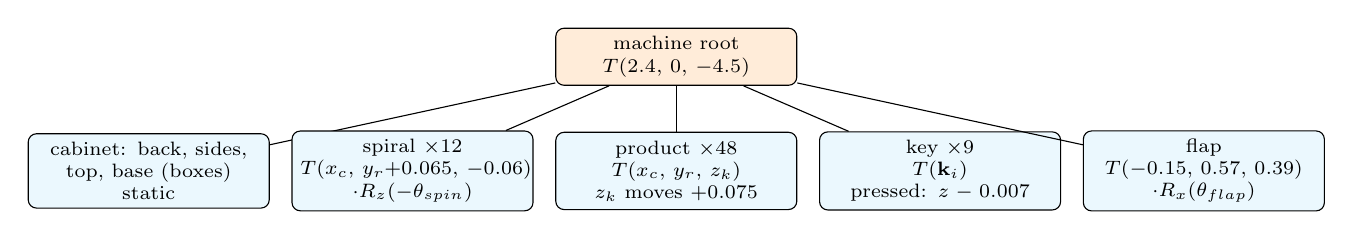
\begin{tikzpicture}[level distance=1.45cm,
  level 1/.style={sibling distance=3.35cm},
  every node/.style={draw,rounded corners=3pt,fill=cyan!8,font=\scriptsize,align=center,inner sep=3pt,text width=2.85cm}]
\node[fill=orange!15] {machine root\\$T(2.4,\,0,\,-4.5)$}
  child {node {cabinet: back, sides,\\top, base (boxes)\\static}}
  child {node {spiral $\times12$\\$T(x_c,\,y_r{+}0.065,\,-0.06)$\\$\cdot R_z(-\theta_{spin})$}}
  child {node {product $\times48$\\$T(x_c,\,y_r,\,z_k)$\\$z_k$ moves $+0.075$}}
  child {node {key $\times9$\\$T(\mathbf{k}_i)$\\pressed: $z-0.007$}}
  child {node {flap\\$T(-0.15,\,0.57,\,0.39)$\\$\cdot R_x(\theta_{flap})$}};
\end{tikzpicture}
\caption{Node tree of the vending machine. Changing $\theta_{spin}$ turns a spiral about its own axis;
changing $\theta_{flap}$ swings the flap about its top edge.}\label{fig:vendtree}
\end{figure}

\emph{Worked example: one vertex of the right side panel, from the unit cube to the world.}
\begin{figure}[H]
\centering
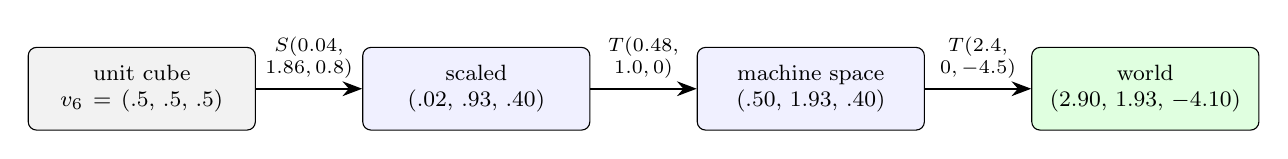
\begin{tikzpicture}[node distance=1.35cm,
  vb/.style={draw,rounded corners=3pt,fill=#1,font=\footnotesize,align=center,minimum height=1.05cm,text width=2.65cm},
  vb/.default=blue!6, lb/.style={font=\scriptsize,above,align=center}]
\node[vb=gray!10] (u) {unit cube\\$v_6=(.5,\,.5,\,.5)$};
\node[vb,right=of u] (s) {scaled\\$(.02,\,.93,\,.40)$};
\node[vb,right=of s] (t) {machine space\\$(.50,\,1.93,\,.40)$};
\node[vb=green!12,right=of t] (w) {world\\$(2.90,\,1.93,\,-4.10)$};
\draw[arr] (u) -- node[lb]{$S(0.04,$\\$1.86,0.8)$} (s);
\draw[arr] (s) -- node[lb]{$T(0.48,$\\$1.0,0)$} (t);
\draw[arr] (t) -- node[lb]{$T(2.4,$\\$0,-4.5)$} (w);
\end{tikzpicture}
\caption{$\mathbf{p}_{world}=T(2.4,0,-4.5)\cdot T(0.48,1.0,0)\cdot S(0.04,1.86,0.8)\cdot\mathbf{v}$ for the corner $v_6$.}\label{fig:vendpipe}
\end{figure}
\begin{table}[H]
\centering\small
\caption{The 8 corners of the vending machine side panel, step by step}\label{tab:vendcorners}
\begin{tabular}{@{}c c c c c@{}}
\toprule
Corner & unit $\mathbf{v}$ & after $S$ & after $T$ (machine space) & world \\ \midrule
$v_0$ & $(-.5,-.5,-.5)$ & $(-.02,-.93,-.40)$ & $(.46,.07,-.40)$ & $(2.86,0.07,-4.90)$ \\
$v_1$ & $(\ .5,-.5,-.5)$ & $(\ .02,-.93,-.40)$ & $(.50,.07,-.40)$ & $(2.90,0.07,-4.90)$ \\
$v_2$ & $(\ .5,\ .5,-.5)$ & $(\ .02,\ .93,-.40)$ & $(.50,1.93,-.40)$ & $(2.90,1.93,-4.90)$ \\
$v_3$ & $(-.5,\ .5,-.5)$ & $(-.02,\ .93,-.40)$ & $(.46,1.93,-.40)$ & $(2.86,1.93,-4.90)$ \\
$v_4$ & $(-.5,-.5,\ .5)$ & $(-.02,-.93,\ .40)$ & $(.46,.07,\ .40)$ & $(2.86,0.07,-4.10)$ \\
$v_5$ & $(\ .5,-.5,\ .5)$ & $(\ .02,-.93,\ .40)$ & $(.50,.07,\ .40)$ & $(2.90,0.07,-4.10)$ \\
$v_6$ & $(\ .5,\ .5,\ .5)$ & $(\ .02,\ .93,\ .40)$ & $(.50,1.93,\ .40)$ & $(2.90,1.93,-4.10)$ \\
$v_7$ & $(-.5,\ .5,\ .5)$ & $(-.02,\ .93,\ .40)$ & $(.46,1.93,\ .40)$ & $(2.86,1.93,-4.10)$ \\
\bottomrule
\end{tabular}
\end{table}
Panel size: $2.86\to2.90$ (4 cm), $0.07\to1.93$ (1.86 m), $-4.90\to-4.10$ (80 cm). The other two machines
use $x=3.7$ and $x=5.0$ in the first translation.

\objhead{Function.} Each machine is a state machine (\Cref{fig:vendsm}). Money is an integer number of Taka.
The user inserts a Tk 10 coin or a Tk 50 note, types a code such as \texttt{B2} (row A--D, column 1--3) and
presses \textbf{OK}. The spiral turns $360^\circ$ in 1.6 s and the products advance by one place (0.075 m).
The front product then falls freely with gravity $g=9.81\,\mathrm{m/s^2}$ and bounces on the tray with a
restitution of 0.32:
\[
v_y \leftarrow v_y - g\,\Delta t,\qquad \mathbf{p}\leftarrow\mathbf{p}+\mathbf{v}\,\Delta t,\qquad
\text{if } p_y < y_{floor}:\ v_y \leftarrow -0.32\,v_y .
\]
When the bounce speed drops below 0.35 m/s the product lies still. Pushing the flap puts it into the
player's bag, the change falls into the coin cup as small coins, and an empty slot is refilled after 40 s.
The LCD, the price tags and the key labels are text drawn on the machine (\Cref{sec:text}).
\begin{figure}[H]
\centering
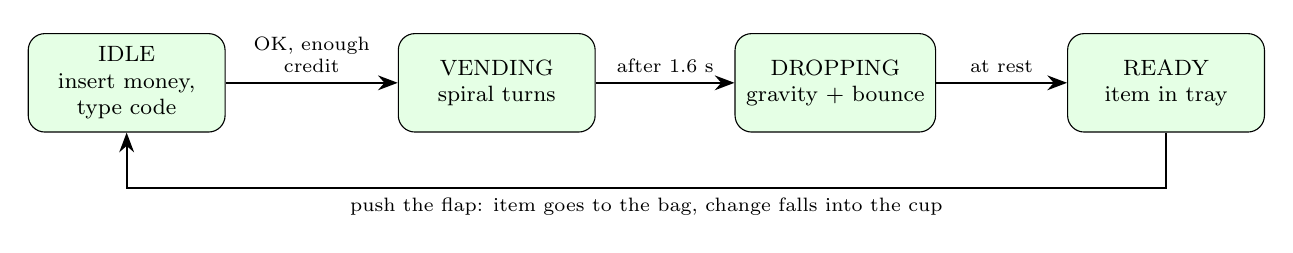
\begin{tikzpicture}[state/.append style={minimum width=2.5cm,minimum height=1.25cm,font=\footnotesize},lb/.style={font=\scriptsize,align=center}]
\node[state] (idle) at (0,0) {IDLE\\insert money,\\type code};
\node[state] (vend) at (4.7,0) {VENDING\\spiral turns};
\node[state] (drop) at (9.0,0) {DROPPING\\gravity + bounce};
\node[state] (ready) at (13.2,0) {READY\\item in tray};
\draw[arr] (idle) -- node[lb,above]{OK, enough\\credit} (vend);
\draw[arr] (vend) -- node[lb,above]{after 1.6 s} (drop);
\draw[arr] (drop) -- node[lb,above]{at rest} (ready);
\draw[arr] (ready.south) -- ++(0,-0.7) -| node[lb,below,pos=0.25]{push the flap: item goes to the bag, change falls into the cup} (idle.south);
\end{tikzpicture}
\caption{Vending machine state machine.}\label{fig:vendsm}
\end{figure}
\objhead{Colours, textures and sound.} Painted body (red, orange or blue), dark metal trims, steel shelves,
polished metal coin plate and spirals, transparent front glass ($\alpha=0.18$), glowing marquee, tube light
and LEDs. Sounds: a coin sound when money is inserted, the motor while the spiral turns, a thud when the
product hits the tray and small coin sounds when the change lands in the cup.

% -----------------------------------------------------------------------------
\subsubsection{Products}
Every machine holds 12 slots with 4 products each. Six product types exist; their colours come from the
product list of each machine (for example Cola red and white, Mango Juice yellow and green).
\objviews[5.6cm]{products}{Products: can, bottle, juice box, chips bag, chocolate bar and cookie box.}
\objhead{Construction.} A \emph{can} is a cylinder body, a coloured band and two metal rims. A \emph{bottle}
adds a truncated-cone shoulder, a neck and a cap. A \emph{chips bag} is a box with a flattened sphere
(``puff'') and two crimp strips; its round logo is a cylinder rotated $R_x(90^\circ)$. A \emph{chocolate bar}
is a box with a narrower band, a \emph{cookie box} a box with a stripe and a round picture, and a
\emph{juice box} a carton with a label and a straw tilted by $R_z(12^\circ)$.
\objhead{Function.} Products sit on the spirals at $z = 0.0525 - 0.075k$ ($k=0\ldots3$) and move forward while
the spiral turns. A dropped product becomes a free body (position, velocity, spin) until it rests in the tray.
\objhead{Colours, textures and sound.} Two colours per product, glossy plastic for bottles, polished metal
for the can rims. Products have no sounds of their own (the drop sound belongs to the machine).

% -----------------------------------------------------------------------------
\subsubsection{ATM}
The ATM is $1.0\times2.08\times0.72$ m and stands at the back wall of the ATM room.
\objviews{atm}{ATM: (a) complete, (b) disconnected parts with their names.}
\begin{table}[H]\centering\footnotesize
\caption{ATM in the world, placed with $M_{place}=T(-9.5, 0, -4.55)$: centre of each key part and the world position $M_{place}\,M_{part}\,\mathbf{v}$ of two of its real mesh vertices A and B (\Cref{tab:vertexpair})}\label{tab:world_atm}
\begin{tabular}{@{}l l c c c@{}}
\toprule
Part & Shape & Centre $(x,y,z)$ & Vertex A & Vertex B \\
\midrule
Plinth & cube & $(-9.50, 0.04, -4.55)$ & $(-10.00, 0.00, -4.91)$ & $(-9.00, 0.08, -4.19)$ \\
Lower cabinet & cube & $(-9.50, 0.54, -4.55)$ & $(-9.98, 0.08, -4.88)$ & $(-9.02, 1.00, -4.22)$ \\
Upper fascia & cube & $(-9.50, 1.45, -4.63)$ & $(-9.98, 1.05, -4.88)$ & $(-9.02, 1.85, -4.38)$ \\
Header & cube & $(-9.50, 1.96, -4.55)$ & $(-10.02, 1.84, -4.91)$ & $(-8.98, 2.08, -4.19)$ \\
Screen & cube & $(-9.50, 1.46, -4.36)$ & $(-9.71, 1.30, -4.36)$ & $(-9.29, 1.62, -4.36)$ \\
Keypad shelf (tilted) (1) & cube & $(-9.50, 1.03, -4.15)$ & $(-9.98, 1.04, -4.30)$ & $(-9.02, 1.03, -4.00)$ \\
Keypad shelf (tilted) (2) & cube & $(-9.50, 1.06, -4.15)$ & $(-9.68, 1.09, -4.27)$ & $(-9.32, 1.04, -4.04)$ \\
Cash dispenser (1) & cube & $(-9.50, 0.88, -4.21)$ & $(-9.70, 0.83, -4.22)$ & $(-9.30, 0.93, -4.21)$ \\
Cash dispenser (2) & cube & $(-9.50, 0.88, -4.20)$ & $(-9.66, 0.86, -4.21)$ & $(-9.34, 0.90, -4.20)$ \\
Card slot (1) & cube & $(-9.16, 1.30, -4.37)$ & $(-9.22, 1.27, -4.38)$ & $(-9.10, 1.33, -4.36)$ \\
Card slot (2) & cube & $(-9.16, 1.30, -4.35)$ & $(-9.21, 1.30, -4.36)$ & $(-9.11, 1.30, -4.35)$ \\
\bottomrule
\end{tabular}
\end{table}

\objhead{Construction.} A plinth, a lower cabinet and an upper fascia (boxes) carry the screen bezel, the
card slot, the receipt slot, the cash dispenser and two privacy wings. The keypad shelf is a child node
tilted towards the user,
\[
M_{keypad} = M_{ATM}\cdot T(0,\,1.035,\,0.40)\cdot R_x(12^\circ),
\]
and the 16 keys are placed in that node on a $4\times4$ grid,
$\mathbf{k}_i = (-0.135 + 0.075\,(i \bmod 4),\ 0.03,\ -0.085 + 0.052\,\lfloor i/4\rfloor)$, so they follow the slope
automatically. A pressed key moves down by 6 mm. The card slides in and out along $z$, four bank notes slide
out of the dispenser, and the receipt is a thin box rotated by $R_x(25^\circ\cdot a)$ while it comes out.
\objhead{Function.} The ATM follows the state machine of \Cref{fig:atmsm}. The PIN is 1234; amounts of
Tk 500, 1,000, 2,000, 5,000 (side keys), fast cash or any other multiple of 100 can be withdrawn. The card is
always returned before the cash, and the cash is added to the player's wallet and taken from the bank
balance. The screen shows every step with rectangles and text, and a panel on the HUD lists the eight steps
(\Cref{sec:interaction}).
\objhead{Colours, textures and sound.} Dark grey cabinet, light grey fascia, blue header with a glowing light
strip, brushed metal keypad plate, coloured CANCEL / CLEAR / ENTER keys, glowing screen. Sounds: a beep for
every key and a cash-counting sound when the notes come out.

% -----------------------------------------------------------------------------
\subsubsection{Coffee machine}
The coffee machine ($0.43\times0.81\times0.40$ m) stands on the counter in the lounge.
\objviews{coffee}{Coffee machine while brewing: (a) complete, (b) disconnected parts with their names.}
\begin{table}[H]\centering\footnotesize
\caption{Coffee machine in the world, placed with $M_{place}=T(-5, 0.92, -4.55)$: centre of each key part and the world position $M_{place}\,M_{part}\,\mathbf{v}$ of two of its real mesh vertices A and B (\Cref{tab:vertexpair})}\label{tab:world_coffee}
\begin{tabular}{@{}l l c c c@{}}
\toprule
Part & Shape & Centre $(x,y,z)$ & Vertex A & Vertex B \\
\midrule
Base & cube & $(-5.00, 0.94, -4.55)$ & $(-5.20, 0.92, -4.75)$ & $(-4.80, 0.96, -4.35)$ \\
Steel column & cube & $(-5.00, 1.24, -4.65)$ & $(-5.20, 0.96, -4.75)$ & $(-4.80, 1.52, -4.55)$ \\
Head unit & cube & $(-5.00, 1.45, -4.55)$ & $(-5.21, 1.37, -4.75)$ & $(-4.79, 1.53, -4.35)$ \\
Bean hopper & truncated cone & $(-5.00, 1.62, -4.61)$ & $(-4.88, 1.71, -4.61)$ & $(-4.92, 1.53, -4.61)$ \\
Drip tray + grill (1) & cube & $(-5.00, 0.97, -4.47)$ & $(-5.14, 0.96, -4.56)$ & $(-4.86, 0.98, -4.38)$ \\
Drip tray + grill (2) & cube & $(-5.11, 0.98, -4.47)$ & $(-5.11, 0.98, -4.55)$ & $(-5.11, 0.98, -4.39)$ \\
Cup & truncated cone & $(-5.00, 1.03, -4.46)$ & $(-4.96, 1.07, -4.46)$ & $(-4.97, 0.98, -4.46)$ \\
\bottomrule
\end{tabular}
\end{table}

\objhead{Construction.} A base, a steel column, two side panels and a head unit form the body. The bean
hopper is a glass truncated cone turned upside down with $R_x(180^\circ)$, so it is wider at the top. The three
round buttons are cylinders rotated $R_x(90^\circ)$ so that their flat face points forward, each with a torus ring.
The cup is also an upside-down truncated cone with a torus handle. The coffee inside the cup is a thin disc whose
height and radius follow the cup's taper:
\[
h = 0.006 + 0.075\,f,\qquad r = 2\,\big(0.0298 + (0.0425-0.0298)\,h/0.09\big) - 0.006,
\]
where $f\in[0,1]$ is the fill level. The pouring stream is a thin cylinder from the nozzle down to the
coffee surface.
\objhead{Function.} The three buttons make an Espresso, a Cappuccino or a Masala Tea:
\texttt{IDLE} $\rightarrow$ \texttt{CUP\_DROP} (0.5 s, the cup falls) $\rightarrow$ \texttt{GRINDING} (1.6 s) $\rightarrow$
\texttt{BREWING} (4.5 s, the cup fills) $\rightarrow$ \texttt{READY}. Steam puffs rise from the cup (\Cref{sec:particles}).
Taking the cup puts the drink into the bag.
\objhead{Colours, textures and sound.} Black body, brushed steel column, glass hopper with brown bean texture,
glowing LCD and status LED (green when idle, orange while busy). Sounds: grinder, pouring and a beep when ready.

% -----------------------------------------------------------------------------
\subsubsection{Television}
The television hangs on the lounge wall at $(0,1.75,-4.86)$.
\objviews[6.5cm]{tv}{Television: (a) complete with the news channel, (b) disconnected parts.}
\begin{table}[H]\centering\footnotesize
\caption{Television in the world, placed with $M_{place}=T(0, 1.75, -4.86)$: centre of each key part and the world position $M_{place}\,M_{part}\,\mathbf{v}$ of two of its real mesh vertices A and B (\Cref{tab:vertexpair})}\label{tab:world_tv}
\begin{tabular}{@{}l l c c c@{}}
\toprule
Part & Shape & Centre $(x,y,z)$ & Vertex A & Vertex B \\
\midrule
Wall bracket & cube & $(0.00, 1.75, -4.92)$ & $(-0.23, 1.59, -4.95)$ & $(0.23, 1.91, -4.89)$ \\
TV body & cube & $(0.00, 1.75, -4.88)$ & $(-0.93, 1.21, -4.90)$ & $(0.93, 2.29, -4.85)$ \\
Screen & cube & $(0.00, 1.75, -4.85)$ & $(-0.89, 1.25, -4.85)$ & $(0.89, 2.25, -4.85)$ \\
Bottom trim & cube & $(0.00, 1.20, -4.86)$ & $(-0.93, 1.19, -4.88)$ & $(0.93, 1.21, -4.83)$ \\
Power LED & sphere & $(0.86, 1.22, -4.84)$ & $(0.86, 1.21, -4.84)$ & $(0.86, 1.22, -4.84)$ \\
\bottomrule
\end{tabular}
\end{table}

\objhead{Construction.} A wall bracket, a body box, a bottom trim, the screen and a power LED. The pictures
are not textures: each channel is drawn every frame on a \emph{canvas} placed on the screen, using
rectangles and text. Circles (heads, the sun, trees, the ball) are drawn as horizontal strips of width
$2\sqrt{r^2-y^2}$, and triangles (mountains) as strips whose width shrinks linearly with the height.
\objhead{Function.} Looking at the screen and pressing E cycles through news (with a moving ticker), nature,
live football and a weather map that shows the in-game time, and off. While it is on, the TV adds a
flickering coloured point light to the room whose colour follows the picture.
\objhead{Colours, textures and sound.} Black body, dark metal bracket, glowing screen, green or red power
LED. A click is heard when the channel changes.

% -----------------------------------------------------------------------------
\subsubsection{Aquarium and fish}
The aquarium ($1.8\times1.45\times0.5$ m) stands in the library.
\objviews{aquarium}{Aquarium: (a) complete, (b) disconnected parts (stand, sand, rocks, plants, glass, water, fish, bubbles).}
\begin{table}[H]\centering\footnotesize
\caption{Aquarium in the world, placed with $M_{place}=T(9.8, 0, 4.45)\,R_y(180^\circ)$: centre of each key part and the world position $M_{place}\,M_{part}\,\mathbf{v}$ of two of its real mesh vertices A and B (\Cref{tab:vertexpair})}\label{tab:world_aquarium}
\begin{tabular}{@{}l l c c c@{}}
\toprule
Part & Shape & Centre $(x,y,z)$ & Vertex A & Vertex B \\
\midrule
Wooden stand & cube & $(9.80, 0.38, 4.45)$ & $(10.70, 0.00, 4.70)$ & $(8.90, 0.75, 4.20)$ \\
Sand bed & cube & $(9.80, 0.79, 4.45)$ & $(10.68, 0.76, 4.68)$ & $(8.92, 0.82, 4.22)$ \\
Water & cube & $(9.80, 1.03, 4.45)$ & $(10.68, 0.78, 4.68)$ & $(8.92, 1.28, 4.22)$ \\
Glass tank & cube & $(9.80, 1.06, 4.45)$ & $(10.70, 0.75, 4.70)$ & $(8.90, 1.37, 4.20)$ \\
Hood & cube & $(9.80, 1.41, 4.45)$ & $(10.72, 1.37, 4.72)$ & $(8.88, 1.45, 4.18)$ \\
Fish bodies (1) & sphere & $(10.19, 1.06, 4.45)$ & $(10.19, 1.04, 4.45)$ & $(10.19, 1.09, 4.45)$ \\
Fish bodies (2) & sphere & $(9.39, 1.12, 4.46)$ & $(9.39, 1.10, 4.46)$ & $(9.39, 1.15, 4.46)$ \\
\bottomrule
\end{tabular}
\end{table}

\objhead{Construction.} A wooden stand with three doors carries a sand bed, rocks (squashed low spheres), a
driftwood branch (low cylinder rotated $R_y(30^\circ)R_z(75^\circ)$), water plants (cross cards), an air stone,
the water volume and the glass tank (two transparent boxes) and a hood with a light strip. Each fish is a node
$T(x,y,z)\cdot R_y(\psi)$ with a sphere body scaled to $(0.45s,0.75s,1.25s)$, a cone tail in a child node that
wags with $R_y(25^\circ\sin(9t+3\varphi))$, a wedge fin and two sphere eyes.
\objhead{Function.} Each of the 7 fish swims on its own ellipse, $x=r_x\cos\varphi$, $z=r_z\sin\varphi$ with
$\varphi \mathrel{+}= \omega\,\Delta t$, and faces its direction of motion, $\psi=\operatorname{atan2}(\Delta x,\Delta z)$.
``Feed the fish'' drops 12 food crumbs that sink slowly; while there is food, every fish swims up to the
surface. Bubbles rise from the air stone and the plants sway (\Cref{sec:effects}).
\objhead{Colours, textures and sound.} Wood texture on the stand, sand texture, rock texture, bark texture on
the driftwood, transparent water ($\alpha=0.16$) and glass, glowing hood light. A click sounds when the fish
are fed.

% =============================================================================
\subsection{Furniture}
% -----------------------------------------------------------------------------
\subsubsection{Sofa}
The sofa function builds a sofa for any number of seats $n$; its width is $W = 0.72n + 0.32$ m. The lounge
has two three-seat sofas and four armchairs.
\objviews{sofa}{Sofa with three seats: (a) complete, (b) disconnected parts.}
\begin{table}[H]\centering\footnotesize
\caption{Sofa (3 seats) in the world, placed with $M_{place}=T(0, 0, -0.6)\,R_y(180^\circ)$: centre of each key part and the world position $M_{place}\,M_{part}\,\mathbf{v}$ of two of its real mesh vertices A and B (\Cref{tab:vertexpair})}\label{tab:world_sofa}
\begin{tabular}{@{}l l c c c@{}}
\toprule
Part & Shape & Centre $(x,y,z)$ & Vertex A & Vertex B \\
\midrule
Base frame & cube & $(0.00, 0.20, -0.60)$ & $(1.24, 0.09, -0.16)$ & $(-1.24, 0.31, -1.04)$ \\
Back frame & cube & $(0.00, 0.56, -0.23)$ & $(1.24, 0.23, -0.15)$ & $(-1.24, 0.89, -0.31)$ \\
Seat cushions (1) & cube & $(0.72, 0.38, -0.65)$ & $(1.07, 0.30, -0.33)$ & $(0.37, 0.46, -0.97)$ \\
Seat cushions (2) & cube & $(0.00, 0.38, -0.65)$ & $(0.35, 0.30, -0.33)$ & $(-0.35, 0.46, -0.97)$ \\
Arm rests (1) & cube & $(1.16, 0.42, -0.60)$ & $(1.24, 0.20, -0.16)$ & $(1.08, 0.64, -1.04)$ \\
Arm rests (2) & cube & $(-1.16, 0.42, -0.60)$ & $(-1.08, 0.20, -0.16)$ & $(-1.24, 0.64, -1.04)$ \\
Legs (1) & cylinder & $(1.16, 0.04, -0.24)$ & $(1.14, 0.00, -0.24)$ & $(1.14, 0.09, -0.24)$ \\
Legs (2) & cylinder & $(1.16, 0.04, -0.96)$ & $(1.14, 0.00, -0.96)$ & $(1.14, 0.09, -0.96)$ \\
\bottomrule
\end{tabular}
\end{table}

\objhead{Construction.} A base frame and a back frame (boxes); per seat a cushion box, a rounded front roll
(cylinder rotated $R_z(90^\circ)$ so that it lies along $x$) and a back cushion tilted by $R_x(-10^\circ)$; two
arm rests made of a box and a rolled cylinder rotated $R_x(90^\circ)$ to lie along $z$; four wooden legs; and
two throw pillows rotated about all three axes.
\objhead{Function.} Visitors can sit on any seat: each seat has a stand point and a sit point. The sitting
pose of a person is described in \Cref{sec:humans}.
\objhead{Colours, textures and sound.} Blue fabric texture (darker on the frame), yellow fabric pillows, wooden
legs. No sound.

% -----------------------------------------------------------------------------
\subsubsection{Armchair}
\objviews[6.5cm]{armchair}{Armchair: (a) complete, (b) disconnected parts.}
\objhead{Construction and function.} The armchair is the sofa function called with $n=1$ (no throw pillows),
which shows how one parametric model produces different objects. Armchairs stand in the lounge and in the
library, where visitors sit and read.
\objhead{Colours, textures and sound.} Brown fabric texture, wooden legs. No sound.

% -----------------------------------------------------------------------------
\subsubsection{Coffee table and rug}
\objviews[6.5cm]{tableset}{Coffee table on its rug: (a) complete, (b) disconnected parts.}
\objhead{Construction.} A wooden top and a lower shelf (boxes), four metal legs placed at
$(\pm(w/2-0.06),\,0.2,\,\pm(d/2-0.06))$, two magazines rotated about $y$, a fruit bowl and three fruits. The bowl
is a hemisphere scaled with a \emph{negative} $y$ factor, $S=(0.24,-0.10,0.24)$, which mirrors it so that it opens
upwards. The rug is two thin boxes: a border and a carpet-textured centre.
\objhead{Colours, textures and sound.} Wood texture, dark metal legs, carpet texture on the rug. No sound.

% -----------------------------------------------------------------------------
\subsubsection{Bookshelf}
\objviews{bookshelf}{Bookshelf: (a) complete, (b) disconnected parts.}
\begin{table}[H]\centering\footnotesize
\caption{Bookshelf in the world, placed with $M_{place}=T(9, 0, -4.69)$: centre of each key part and the world position $M_{place}\,M_{part}\,\mathbf{v}$ of two of its real mesh vertices A and B (\Cref{tab:vertexpair})}\label{tab:world_bookshelf}
\begin{tabular}{@{}l l c c c@{}}
\toprule
Part & Shape & Centre $(x,y,z)$ & Vertex A & Vertex B \\
\midrule
Side boards (1) & cube & $(8.12, 1.15, -4.69)$ & $(8.10, 0.00, -4.88)$ & $(8.14, 2.30, -4.50)$ \\
Side boards (2) & cube & $(9.88, 1.15, -4.69)$ & $(9.86, 0.00, -4.88)$ & $(9.90, 2.30, -4.50)$ \\
Top board & cube & $(9.00, 2.28, -4.69)$ & $(8.10, 2.26, -4.88)$ & $(9.90, 2.30, -4.50)$ \\
Back board & cube & $(9.00, 1.15, -4.87)$ & $(8.10, 0.00, -4.88)$ & $(9.90, 2.30, -4.86)$ \\
Shelves (1) & cube & $(9.00, 0.10, -4.69)$ & $(8.13, 0.09, -4.87)$ & $(9.87, 0.11, -4.51)$ \\
Shelves (2) & cube & $(9.00, 0.54, -4.69)$ & $(8.13, 0.52, -4.87)$ & $(9.87, 0.55, -4.51)$ \\
Plinth & cube & $(9.00, 0.05, -4.69)$ & $(8.10, 0.00, -4.88)$ & $(9.90, 0.10, -4.50)$ \\
\bottomrule
\end{tabular}
\end{table}

\objhead{Construction.} Two side boards, a top, a back board, a plinth and five shelves. The books are not
modelled one by one: each row is a plain box (the colour of the pages) with a quad in front that carries the
generated \emph{books} texture. Each shelf has two rows of different widths, and on every second shelf one
quad is mirrored with a negative $x$ scale, so the pattern does not repeat. One book leans by $R_z(-12^\circ)$.
\objhead{Function.} Visitors stand in front of the shelves and browse.
\objhead{Colours, textures and sound.} Wood texture, books texture, plain page colour. No sound.

% -----------------------------------------------------------------------------
\subsubsection{Reading table and chair}
\objviews[6.5cm]{reading}{Reading table and chair: (a) complete, (b) disconnected parts.}
\objhead{Construction.} The table is a round top, a pedestal and a foot disc (cylinders) with a book box
rotated by $R_y(20^\circ)$. The chair is a seat box, a backrest tilted by $R_x(-6^\circ)$ and four legs at
$(\pm0.19,\,0.21,\,\pm0.19)$; in the figure the chair node is turned by $R_y(180^\circ)$ to face the table.
\objhead{Colours, textures and sound.} Wood texture, dark metal pedestal, red fabric seat. No sound.

% -----------------------------------------------------------------------------
\subsubsection{Wall clock}
Three clocks hang in the building; their hands show the in-game time.
\objviews[6.0cm]{clock}{Wall clock: (a) complete, (b) disconnected parts.}
\begin{table}[H]\centering\footnotesize
\caption{Wall clock in the world, placed with $M_{place}=T(0, 3, -4.87)$: centre of each key part and the world position $M_{place}\,M_{part}\,\mathbf{v}$ of two of its real mesh vertices A and B (\Cref{tab:vertexpair})}\label{tab:world_clock}
\begin{tabular}{@{}l l c c c@{}}
\toprule
Part & Shape & Centre $(x,y,z)$ & Vertex A & Vertex B \\
\midrule
Wooden rim & torus & $(0.00, 3.00, -4.85)$ & $(0.21, 3.00, -4.85)$ & $(0.13, 3.00, -4.85)$ \\
Clock face & cylinder & $(0.00, 3.00, -4.86)$ & $(0.18, 3.00, -4.87)$ & $(0.18, 3.00, -4.84)$ \\
Hour hand & cube & $(-0.04, 3.03, -4.83)$ & $(0.00, 2.99, -4.84)$ & $(-0.08, 3.06, -4.83)$ \\
Minute hand & cube & $(0.04, 3.06, -4.83)$ & $(-0.01, 3.00, -4.83)$ & $(0.09, 3.11, -4.83)$ \\
Centre cap & cylinder & $(0.00, 3.00, -4.83)$ & $(0.01, 3.00, -4.83)$ & $(0.01, 3.00, -4.82)$ \\
\bottomrule
\end{tabular}
\end{table}

\objhead{Construction.} A torus rim and a face disc, both rotated $R_x(90^\circ)$ to face forward. Each of the
12 ticks is a box in its own node rotated by $R_z(-30^\circ\,i)$, so the same box is repeated around the face.
The hands are boxes in nodes rotated by
\[
\theta_{hour} = -30^\circ\cdot(h \bmod 12),\qquad \theta_{minute} = -6^\circ\cdot m,
\]
where $h$ is the in-game hour (with fraction) and $m$ the minutes.
\objhead{Colours, textures and sound.} Wooden rim, light face, dark ticks and hands, red centre cap. No sound.

% -----------------------------------------------------------------------------
\subsubsection{Pendant lamp}
\objviews[6.5cm]{pendant}{Pendant lamp: (a) complete, (b) disconnected parts.}
\objhead{Construction.} A ceiling disc, a cord (thin cylinder), a shade (truncated cone), a diffuser disc and a
bulb sphere. The lamp node is placed at the ceiling point and every part hangs below it, so the cord length is
one parameter.
\objhead{Function.} Each lamp belongs to a light group. When the group is on, the bulb and the diffuser glow
and a point light is placed at the bulb (\Cref{sec:lighting}).
\objhead{Colours, textures and sound.} Dark (lounge) or bronze (library) shade, glowing bulb. No sound.

% -----------------------------------------------------------------------------
\subsubsection{Table lamp and floor lamp}
\objviews[6.5cm]{lamps}{Table lamp on a side table, and a floor lamp: (a) complete, (b) disconnected parts.}
\objhead{Construction.} The table lamp is a ceramic base (sphere), a stem and a fabric shade (truncated cone);
the side table is a round top, a stem and a foot disc. The floor lamp is a base disc, a 1.6 m pole, a shade
and a bulb.
\objhead{Function.} The table lamps belong to the lounge light group; the floor lamp is the reading lamp of the
library and belongs to the spot-light group. When on, the shades glow warm white.
\objhead{Colours, textures and sound.} Fabric shades, dark metal, polished metal stem. No sound.

% -----------------------------------------------------------------------------
\subsubsection{Potted plants}
\objviews[6.5cm]{plants}{The three potted plants: (a) complete, (b) disconnected parts.}
\objhead{Construction.} Every pot is a truncated cone turned upside down ($R_x(180^\circ)$) with a soil disc.
Variant 0 has a stem, a dark core sphere and five leaf cards turned by $R_y(72^\circ\,i)$; variant 1 has six fern
fronds (quads tilted $R_x(35^\circ)$ and turned $R_y(60^\circ\,i)$) and a cross card; variant 2 (snake plant)
has seven thin cones turned by $R_y(51^\circ\,i)$ and tilted $\pm6^\circ$.
\objhead{Colours, textures and sound.} White or terracotta pots, leaf, fern and plain green materials. No sound.

% -----------------------------------------------------------------------------
\subsubsection{Counter and wall cabinet}
\objviews[6.5cm]{counter}{Kitchen counter with a wall cabinet: (a) complete, (b) disconnected parts.}
\objhead{Construction.} The counter is a cabinet body, a black toe kick, a marble top and $\max(2,\lfloor w/0.6\rfloor)$
doors with handles; the handles alternate between the left and right edge of the doors. The wall cabinet
uses the same rule. The coffee machine stands on this counter.
\objhead{Colours, textures and sound.} Wood texture, marble texture, polished metal handles. No sound.

% -----------------------------------------------------------------------------
\subsubsection{Bench}
\objviews[6.0cm]{bench}{Outdoor bench: (a) complete, (b) disconnected parts.}
\objhead{Construction.} Two metal side frames, two back supports tilted by $R_x(-10^\circ)$, four seat slats and
two back slats with the same tilt. Two benches stand on the sidewalk.
\objhead{Colours, textures and sound.} Wood texture slats, dark metal frame. No sound.

% -----------------------------------------------------------------------------
\subsubsection{Waste bin}
\objviews[6.0cm]{bin}{Waste bin: (a) complete, (b) disconnected parts.}
\objhead{Construction.} A cylinder body, a hemisphere lid, a box for the opening and a foot ring. Bins stand
outside next to the benches and inside the building.
\objhead{Colours, textures and sound.} Polished stainless steel, which shows a bright specular highlight
(\Cref{sec:lighting}). No sound.

% -----------------------------------------------------------------------------
\subsubsection{Light switch}
\objviews[5.5cm]{switch}{Light switch: (a) complete, (b) disconnected parts.}
\objhead{Construction.} A plate, a rocker tilted by $R_x(\mp15^\circ)$ depending on the state, and an indicator
LED sphere.
\objhead{Function.} Six switches on the walls control the light groups (lounge, spot lights, ATM room,
library, outdoor). Looking at a switch highlights it; pressing E toggles its group and the rocker flips
(\Cref{sec:interaction}).
\objhead{Colours, textures and sound.} White plastic, green LED when on and red when off. A click is heard.

% -----------------------------------------------------------------------------
\subsubsection{Security camera}
\objviews[5.5cm]{camera}{Security camera: (a) complete, (b) disconnected parts.}
\objhead{Construction.} A wall mount, an arm tilted by $R_x(20^\circ)$ and a camera node
$T(0,-0.10,0.24)\cdot R_x(25^\circ)\,R_y(30^\circ\sin 0.4t)$ that holds the body, the lens and a recording LED.
\objhead{Function.} The camera slowly pans left and right; its LED blinks once per second.
\objhead{Colours, textures and sound.} White plastic, black lens, red glowing LED. No sound.

% -----------------------------------------------------------------------------
\subsubsection{Paintings}
\objviews[5.0cm]{painting}{The three wall paintings: (a) complete, (b) disconnected parts.}
\objhead{Construction.} A wooden frame box and a picture made of flat shapes: a landscape (sky, hills as a
hemisphere rotated $R_x(90^\circ)$, a sun disc), abstract blocks, and a jungle sunset with five flattened cones
as trees.
\objhead{Colours, textures and sound.} Matte colours, wood frame. No sound.

% -----------------------------------------------------------------------------
\subsubsection{Sliding entrance doors}
\objviews[6.5cm]{doors}{Automatic sliding doors (closed): (a) complete, (b) disconnected parts.}
\begin{table}[H]\centering\footnotesize
\caption{Sliding doors in the world, placed with $M_{place}=T(0, 0, 5.18)$: centre of each key part and the world position $M_{place}\,M_{part}\,\mathbf{v}$ of two of its real mesh vertices A and B (\Cref{tab:vertexpair})}\label{tab:world_doors}
\begin{tabular}{@{}l l c c c@{}}
\toprule
Part & Shape & Centre $(x,y,z)$ & Vertex A & Vertex B \\
\midrule
Glass pane (1) & cube & $(-0.60, 1.30, 5.18)$ & $(-1.20, 0.08, 5.17)$ & $(0.00, 2.52, 5.19)$ \\
Glass pane (2) & cube & $(0.60, 1.30, 5.18)$ & $(0.00, 0.08, 5.17)$ & $(1.20, 2.52, 5.19)$ \\
Top and bottom rails (1) & cube & $(-0.60, 2.55, 5.18)$ & $(-1.22, 2.50, 5.16)$ & $(0.02, 2.60, 5.21)$ \\
Top and bottom rails (2) & cube & $(-0.60, 0.05, 5.18)$ & $(-1.22, 0.00, 5.16)$ & $(0.02, 0.10, 5.21)$ \\
Edge posts (1) & cube & $(0.00, 1.30, 5.18)$ & $(-0.02, 0.10, 5.16)$ & $(0.02, 2.50, 5.21)$ \\
Edge posts (2) & cube & $(0.00, 1.30, 5.18)$ & $(-0.02, 0.10, 5.16)$ & $(0.02, 2.50, 5.21)$ \\
Handles (1) & cube & $(-0.10, 1.05, 5.22)$ & $(-0.12, 0.80, 5.21)$ & $(-0.09, 1.30, 5.24)$ \\
Handles (2) & cube & $(0.10, 1.05, 5.22)$ & $(0.09, 0.80, 5.21)$ & $(0.12, 1.30, 5.24)$ \\
\bottomrule
\end{tabular}
\end{table}

\objhead{Construction.} Each leaf is a glass pane, a top and a bottom rail, an edge post and a handle. The left
leaf is drawn in the node $T(-x_{off},0,z)$ and the right leaf in $T(+x_{off},0,z)$, with
\[
x_{off} = 0.6 + 1.15\cdot o,
\]
where $o\in[0,1]$ is the opening.
\objhead{Function.} The doors open while a person (the player or a visitor) is within $2.2\times2.8$ m of the
entrance, $o$ moving towards its target at 1.6 per second. While they are closed they block the way.
\objhead{Colours, textures and sound.} Transparent glass, dark metal rails, polished metal handles. A short
whoosh is heard when the doors start to move.

% -----------------------------------------------------------------------------
\subsubsection{Ceiling and roof fixtures}
\objviews[5.5cm]{fixtures}{Roof air conditioner, recessed spot light, tube light and smoke detector (the ceiling fixtures are turned to face the viewer): (a) complete, (b) disconnected parts.}
\objhead{Construction.} The air conditioner is a casing box, a fan opening (disc), a torus fan guard and a
grille. The spot light is a torus ring around a glowing lens; the tube light is a housing box with two glowing
tubes (cylinders rotated $R_z(90^\circ)$); the smoke detector is a disc with a small LED.
\objhead{Function.} Spot and tube lights glow when their light group is on and carry the spot and point lights
of the rooms.
\objhead{Colours, textures and sound.} Light grey plastic, polished metal rings, glowing lenses. No sound.

% -----------------------------------------------------------------------------
\subsubsection{Street lamp and bollard}
\objviews{streetlamp}{Street lamp and a sidewalk bollard: (a) complete, (b) disconnected parts.}
\begin{table}[H]\centering\footnotesize
\caption{Street lamp + bollard in the world, placed with $M_{place}=T(-18, 0, 8.25)$: centre of each key part and the world position $M_{place}\,M_{part}\,\mathbf{v}$ of two of its real mesh vertices A and B (\Cref{tab:vertexpair})}\label{tab:world_streetlamp}
\begin{tabular}{@{}l l c c c@{}}
\toprule
Part & Shape & Centre $(x,y,z)$ & Vertex A & Vertex B \\
\midrule
Concrete base & cylinder & $(-18.00, 0.15, 8.25)$ & $(-17.83, 0.00, 8.25)$ & $(-17.83, 0.30, 8.25)$ \\
Tapered pole & truncated cone & $(-18.00, 2.90, 8.25)$ & $(-17.91, 0.00, 8.25)$ & $(-17.94, 5.80, 8.25)$ \\
Arm & cylinder & $(-18.00, 5.75, 8.80)$ & $(-17.97, 5.75, 8.25)$ & $(-17.97, 5.75, 9.35)$ \\
Lamp head & tapered box & $(-18.00, 5.74, 9.40)$ & $(-18.19, 5.81, 9.71)$ & $(-17.87, 5.67, 9.21)$ \\
Glowing lens & cube & $(-18.00, 5.66, 9.40)$ & $(-18.15, 5.65, 9.15)$ & $(-17.85, 5.67, 9.65)$ \\
\bottomrule
\end{tabular}
\end{table}

\objhead{Construction.} The street lamp is a concrete base, a tapered pole (truncated cone) of height
$h=5.8$ m, an arm (cylinder rotated $R_x(90^\circ)$), a lamp head (tapered box rotated $R_x(180^\circ)$ so that it
is wider at the top) and a glowing lens. The bollard is a post, a light ring and a hemisphere cap.
\objhead{Function.} The outdoor lamps switch on automatically at dusk. Each street lamp carries a point light that stays
on at any distance.
\objhead{Colours, textures and sound.} Concrete texture, dark metal, warm sodium-coloured glow. No sound.

% -----------------------------------------------------------------------------
\subsubsection{The building}
\begin{figure}[H]
\centering
\begin{minipage}{0.52\linewidth}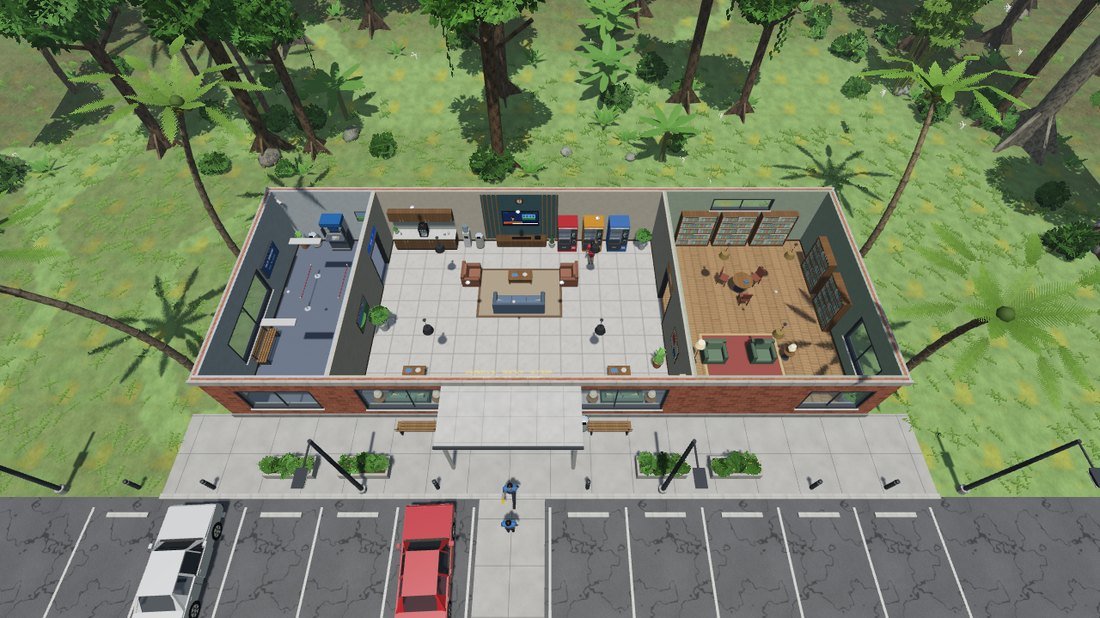
\includegraphics[width=\linewidth]{cutaway_day}\end{minipage}\hfill
\begin{minipage}{0.45\linewidth}
\centering
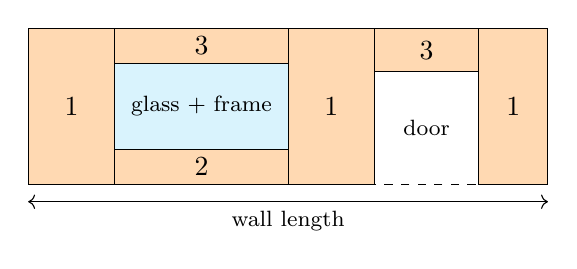
\begin{tikzpicture}[x=0.55cm,y=0.55cm]
\draw[fill=orange!30] (0,0) rectangle (2,3.6); \node at (1,1.8) {1};
\draw[fill=orange!30] (2,0) rectangle (6,0.8); \node at (4,0.4) {2};
\draw[fill=cyan!15] (2,0.8) rectangle (6,2.8); \node[font=\footnotesize] at (4,1.8) {glass + frame};
\draw[fill=orange!30] (2,2.8) rectangle (6,3.6); \node at (4,3.2) {3};
\draw[fill=orange!30] (6,0) rectangle (8,3.6); \node at (7,1.8) {1};
\draw[fill=orange!30] (8,2.6) rectangle (10.4,3.6); \node at (9.2,3.1) {3};
\draw[dashed] (8,0) rectangle (10.4,2.6); \node[font=\footnotesize] at (9.2,1.3) {door};
\draw[fill=orange!30] (10.4,0) rectangle (12,3.6); \node at (11.2,1.8) {1};
\draw[<->] (0,-0.4) -- (12,-0.4) node[midway,below,font=\footnotesize]{wall length};
\end{tikzpicture}
\end{minipage}
\caption{Left: the building with the roof hidden. Right: a wall with one window and one door is split into
(1) full pieces, (2) a piece below the window and (3) pieces above the openings.}\label{fig:wall}
\end{figure}
\objhead{Construction.} All walls are made by one function, \texttt{buildWall()}, which takes a straight wall
and a list of openings and splits the wall into boxes: full-height pieces between openings, a piece below each
window, a lintel above each opening, and for a window a glass pane, an aluminium frame (four bars and a
mullion) and a marble sill; for a door, frame trims. Every piece has two half-thickness layers: brick outside
and plaster inside, in the colour of the room (beige lounge, light blue ATM room, sage green library). Wooden
skirting boards run along the floor. The floors are tiles (lounge), carpet (ATM room) and wood (library).
The roof, the parapet, two air conditioners and the sign board are drawn per frame, so that the roof can be
hidden in the cut-away view.
\objhead{Colours, textures and sound.} Brick, plaster, floor tile, carpet, wood, ceiling tile, roof and
concrete textures.

% =============================================================================
\subsection{People}\label{sec:humans}
There are two types of person, a man and a woman, built by the same function with the same hierarchy
(\Cref{fig:humangraph}); only a few sizes, the hair style and the colours differ. The player's own body is the man.
\begin{figure}[H]
\centering
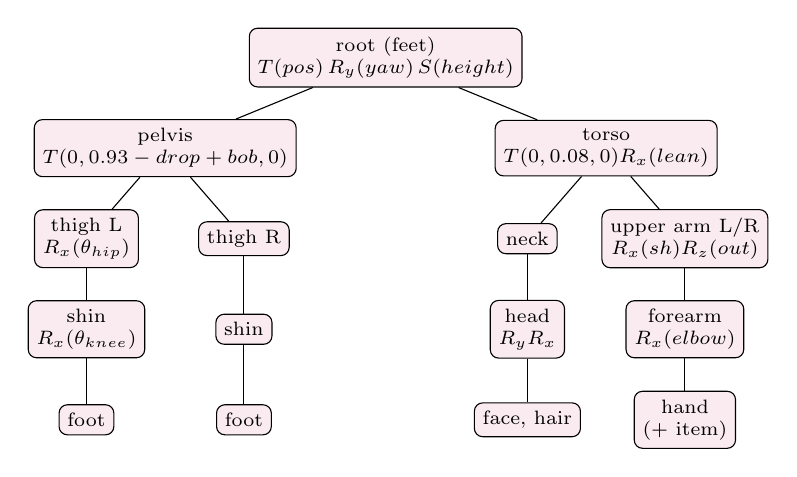
\begin{tikzpicture}[level distance=1.15cm,
  level 1/.style={sibling distance=5.6cm},level 2/.style={sibling distance=2.0cm},level 3/.style={sibling distance=1.9cm},
  every node/.style={draw,rounded corners=3pt,fill=purple!8,font=\scriptsize,align=center,inner sep=3pt}]
\node {root (feet)\\$T(pos)\,R_y(yaw)\,S(height)$}
  child {node {pelvis\\$T(0,0.93-drop+bob,0)$}
     child {node {thigh L\\$R_x(\theta_{hip})$} child {node {shin\\$R_x(\theta_{knee})$} child {node {foot}}}}
     child {node {thigh R} child {node {shin} child {node{foot}}}}}
  child {node {torso\\$T(0,0.08,0)R_x(lean)$}
     child {node {neck} child {node {head\\$R_y R_x$} child {node{face, hair}}}}
     child {node {upper arm L/R\\$R_x(sh)R_z(out)$} child {node {forearm\\$R_x(elbow)$} child {node{hand\\(+ item)}}}}};
\end{tikzpicture}
\caption{Scene graph of a person. A pose only changes the joint angles; every body part stays attached to its parent.}\label{fig:humangraph}
\end{figure}

% -----------------------------------------------------------------------------
\subsubsection{Man}
\objviews{human_walk}{The man (standing): (a) complete, (b) disconnected parts with their names.}
\begin{table}[H]\centering\footnotesize
\caption{Man in the world, placed with $M_{place}=T(0, 0, 6)\,R_y(180^\circ)$: centre of each key part and the world position $M_{place}\,M_{part}\,\mathbf{v}$ of two of its real mesh vertices A and B (\Cref{tab:vertexpair})}\label{tab:world_human_walk}
\begin{tabular}{@{}l l c c c@{}}
\toprule
Part & Shape & Centre $(x,y,z)$ & Vertex A & Vertex B \\
\midrule
Pelvis & cylinder & $(0.00, 0.95, 6.00)$ & $(-0.17, 0.86, 6.00)$ & $(-0.17, 1.04, 6.00)$ \\
Chest & tapered box & $(0.00, 1.31, 6.00)$ & $(-0.21, 1.46, 6.12)$ & $(0.15, 1.16, 5.93)$ \\
Head & sphere & $(0.00, 1.64, 6.00)$ & $(0.00, 1.52, 6.00)$ & $(0.00, 1.76, 6.00)$ \\
Thighs (1) & truncated cone & $(0.09, 0.68, 6.00)$ & $(0.01, 0.90, 6.00)$ & $(0.03, 0.45, 6.00)$ \\
Thighs (2) & truncated cone & $(-0.09, 0.68, 6.00)$ & $(-0.18, 0.90, 6.00)$ & $(-0.15, 0.45, 6.00)$ \\
Shins (1) & truncated cone & $(0.09, 0.24, 6.00)$ & $(0.02, 0.45, 6.00)$ & $(0.04, 0.03, 6.00)$ \\
Shins (2) & truncated cone & $(-0.09, 0.24, 6.00)$ & $(-0.16, 0.45, 6.00)$ & $(-0.14, 0.03, 6.00)$ \\
Upper arms (1) & truncated cone & $(0.24, 1.29, 6.00)$ & $(0.17, 1.42, 6.00)$ & $(0.22, 1.14, 6.00)$ \\
Upper arms (2) & truncated cone & $(-0.24, 1.29, 6.00)$ & $(-0.28, 1.44, 6.00)$ & $(-0.29, 1.15, 6.00)$ \\
Shoes (1) & cube & $(0.09, 0.01, 5.96)$ & $(0.15, -0.03, 6.08)$ & $(0.04, 0.04, 5.83)$ \\
Shoes (2) & cylinder & $(0.09, 0.01, 5.83)$ & $(0.04, 0.04, 5.83)$ & $(0.15, 0.04, 5.83)$ \\
\bottomrule
\end{tabular}
\end{table}

\objhead{Construction.} Every joint is a sphere and every limb a truncated cone. The cones are flipped with
$R_x(180^\circ)$, so the legs are thicker at the hip and the arms thicker at the shoulder. The chest is a tapered
box rotated by $R_z(180^\circ)$ (wide at the shoulders), the waist an elliptic cylinder. The face has sphere eyes,
pupils, nose, ears and jaw and box eyebrows and mouth; the short hair is a hemisphere and a sphere.

\emph{Worked example: the knee.} The knee of the left leg is found by following the chain of nodes:
\[
\mathbf{p}_{knee} = \underbrace{T(\mathbf{p})R_y(\psi)}_{\text{person}}\cdot
\underbrace{T(0,0.93,0)}_{\text{pelvis}}\cdot
\underbrace{T(0.092,-0.03,0)\,R_x(\theta_{thigh})}_{\text{hip}}\cdot
\underbrace{T(0,-0.45,0)}_{\text{knee}}\cdot(0,0,0,1)^T,
\]
with $R_x(\theta):(x,y,z)\mapsto(x,\ y\cos\theta - z\sin\theta,\ y\sin\theta + z\cos\theta)$. In person space:
\begin{itemize}
  \item standing, $\theta_{thigh}=0$: knee at $(0.092,\ 0.90-0.45,\ 0) = (0.092,\ 0.45,\ 0)$;
  \item walking, leg forward, $\theta_{thigh}=-26^\circ$: $(0.092,\ 0.90-0.45\cos26^\circ,\ 0.45\sin26^\circ) = (0.092,\ 0.496,\ 0.197)$.
\end{itemize}
The knee moves 20 cm forward and 4.6 cm up, and the shin and the foot follow because they are its children.

\objhead{Function (animation).} Only the joint angles change. For walking with the phase $\varphi$
($\varphi \mathrel{+}= 7\,\Delta t$):
\[
\theta_{thigh}^{L,R} = \mp 26^\circ\sin\varphi,\quad
\theta_{knee}^{L} = 38^\circ\max(0,\cos\varphi)+4^\circ,\quad
\theta_{shoulder}^{L,R} = \pm22^\circ\sin\varphi,\quad
bob = 0.035\,(1-|\sin\varphi|).
\]
Sitting lowers the pelvis by 0.44 m, turns the thighs by $-88^\circ$ and bends the knees by $88^\circ$. Driving,
pressing buttons and bending down are further fixed poses. Every angle is blended linearly over 0.35 s, so
changes between poses are smooth.
\objhead{Colours, textures and sound.} Skin colour, blue fabric shirt, dark fabric trousers, dark shoes with
white soles, black hair. Footsteps are silent.

% -----------------------------------------------------------------------------
\subsubsection{Woman}
\objviews{human}{The woman holding a coffee cup: (a) complete, (b) disconnected parts with their names.}
\objhead{Construction.} The same hierarchy with a root scale $S(0.95)$ and a width factor $w=0.94$ (her hip is at
$x=0.092\cdot0.94=0.086$). The long hair adds a tall flattened sphere behind the head. She wears a kurta: the
pelvis uses the shirt colour and a hem (an upside-down truncated cone) covers the upper legs. A held item (cup,
can, snack or phone) is a child of the right hand.
\begin{figure}[H]
\centering
\begin{subfigure}{0.3\linewidth}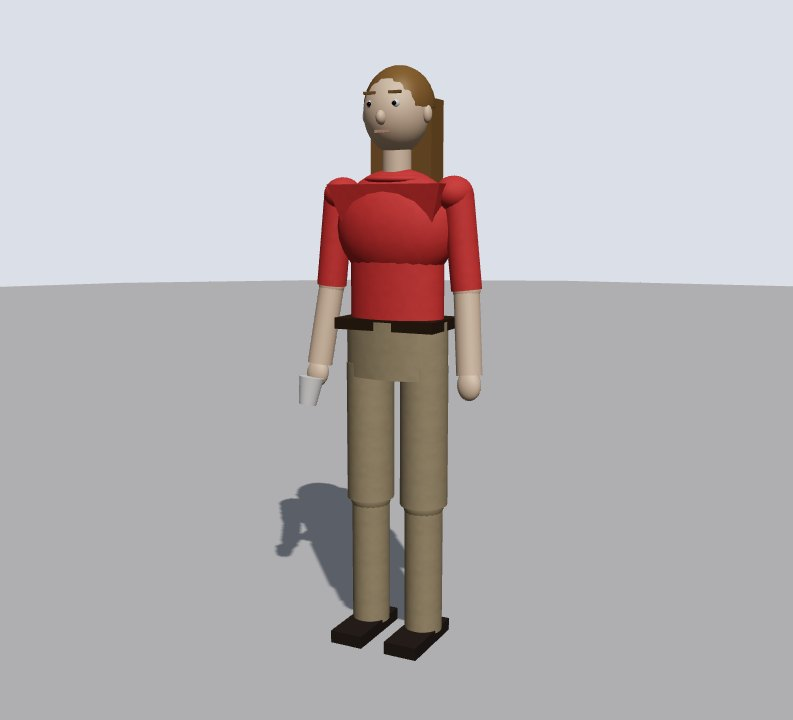
\includegraphics[width=\linewidth]{obj_human}\caption{Standing with a cup}\end{subfigure}
\begin{subfigure}{0.3\linewidth}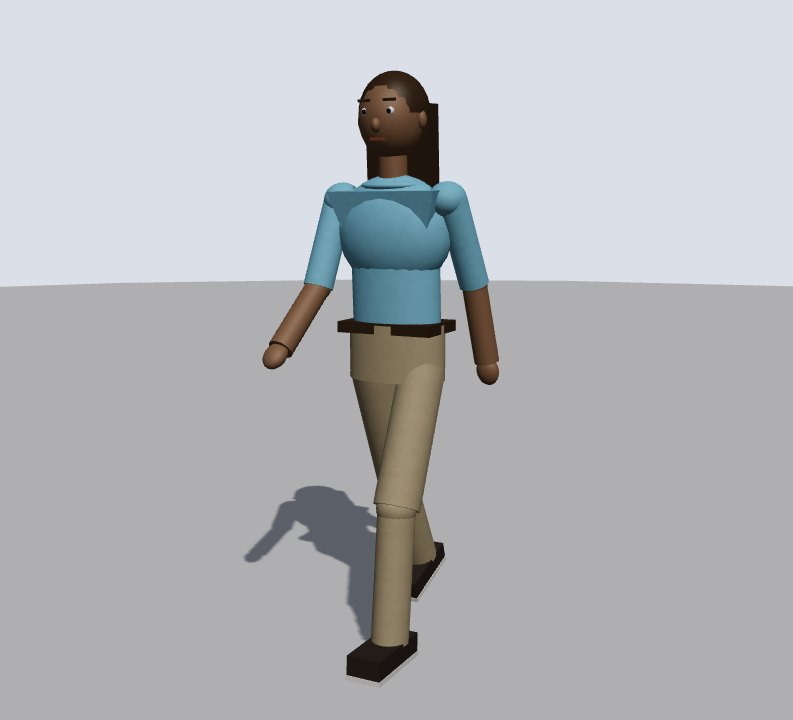
\includegraphics[width=\linewidth]{obj_human_walk}\caption{Walking pose}\end{subfigure}
\begin{subfigure}{0.3\linewidth}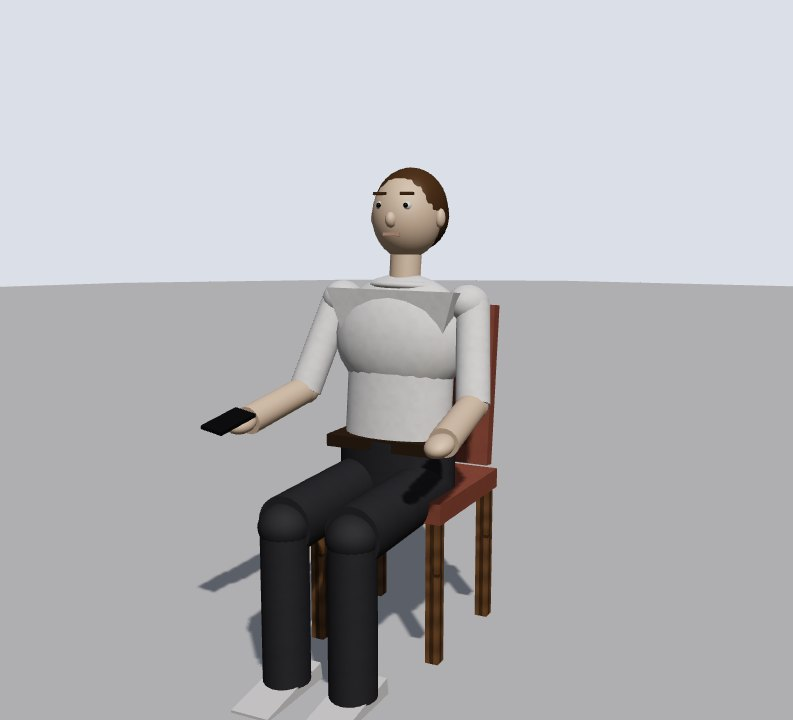
\includegraphics[width=\linewidth]{obj_human_sit}\caption{Sitting on a chair}\end{subfigure}
\caption{Poses produced by the same hierarchical model.}
\end{figure}
\objhead{Colours, textures and sound.} Red kurta, light trousers, brown shoes, long black hair.

% =============================================================================
\subsection{Car}
There is one car model, a sedan of $4.4\times1.78\times1.42$ m, painted red, blue or white.
\objviews[6.5cm]{car_red}{The car (driver door open $55^\circ$, front wheels steered $18^\circ$): (a) complete with its driver, (b) disconnected parts.}
\begin{table}[H]\centering\footnotesize
\caption{Car in the world, placed with $M_{place}=T(-3, 0, 11.2)$: centre of each key part and the world position $M_{place}\,M_{part}\,\mathbf{v}$ of two of its real mesh vertices A and B (\Cref{tab:vertexpair})}\label{tab:world_car_red}
\begin{tabular}{@{}l l c c c@{}}
\toprule
Part & Shape & Centre $(x,y,z)$ & Vertex A & Vertex B \\
\midrule
Front block & cube & $(-3.00, 0.58, 12.64)$ & $(-3.89, 0.30, 11.93)$ & $(-2.11, 0.86, 13.35)$ \\
Rear block & cube & $(-3.00, 0.58, 9.99)$ & $(-3.89, 0.30, 9.05)$ & $(-2.11, 0.86, 10.93)$ \\
Roof & cube & $(-3.00, 1.39, 11.00)$ & $(-3.59, 1.36, 10.29)$ & $(-2.41, 1.42, 11.71)$ \\
Bonnet (wedge) & wedge & $(-3.00, 0.90, 12.78)$ & $(-3.86, 0.86, 13.35)$ & $(-2.14, 0.94, 12.20)$ \\
Windscreen & cube & $(-3.00, 1.12, 11.92)$ & $(-3.57, 0.86, 12.15)$ & $(-2.43, 1.38, 11.69)$ \\
Tyres (1) & cylinder & $(-3.78, 0.32, 12.53)$ & $(-3.68, 0.64, 12.49)$ & $(-3.88, 0.64, 12.56)$ \\
Tyres (2) & cylinder & $(-2.22, 0.32, 12.53)$ & $(-2.12, 0.64, 12.49)$ & $(-2.32, 0.64, 12.56)$ \\
Driver door (1) & cube & $(-4.32, 0.58, 11.65)$ & $(-4.74, 0.32, 11.38)$ & $(-3.90, 0.85, 11.92)$ \\
Driver door (2) & cube & $(-4.30, 0.58, 11.62)$ & $(-4.70, 0.33, 11.36)$ & $(-3.90, 0.83, 11.88)$ \\
\bottomrule
\end{tabular}
\end{table}

\objhead{Construction.} The body is a front block and a rear block (boxes), a passenger-side skin and a floor,
with a rounded nose (cylinder rotated $R_z(90^\circ)$), bumpers and an underbody. The bonnet is a wedge sloping to
the front. The windscreen, the rear window and the side windows are thin parallelograms and triangles built
directly from their corner points (\Cref{sec:transform}); pillars are beams between two points. Inside are
seats, a rear bench, a dashboard and a steering wheel (torus rotated $R_x(70^\circ)$).

\emph{Worked example: a tyre.} The tyre is a cylinder with $S=(0.64,0.22,0.64)$ rotated by $R_z(90^\circ)$, so its
axis points sideways, inside the wheel node $T(-0.78,0.32,1.325)$. With $R_z(90^\circ):(x,y,z)\mapsto(-y,x,z)$:
\begin{table}[H]
\centering\small
\caption{Three vertices of the front tyre (car space)}
\begin{tabular}{@{}l c c c c@{}}
\toprule
Vertex & unit $\mathbf{p}$ & after $S$ & after $R_z(90^\circ)$ & after wheel $T$ \\ \midrule
$\mathbf{p}_0^{top}$ & $(0.5,0.5,0)$ & $(0.32,0.11,0)$ & $(-0.11,0.32,0)$ & $(-0.89,0.64,1.325)$ \\
$\mathbf{p}_0^{bot}$ & $(0.5,-0.5,0)$ & $(0.32,-0.11,0)$ & $(0.11,0.32,0)$ & $(-0.67,0.64,1.325)$ \\
$\mathbf{p}_6^{top}$ & $(0,0.5,0.5)$ & $(0,0.11,0.32)$ & $(-0.11,0,0.32)$ & $(-0.89,0.32,1.645)$ \\
\bottomrule
\end{tabular}
\end{table}
The top of the tyre is at $y=0.64$, twice the wheel radius, so the tyre touches the ground at $y=0$. When the
car moves, the spin $R_x(\theta_{spin})$, the steering $R_y(\delta)$ (front wheels) and the car's own
$T(\mathbf{p}_{car})R_y(\psi)$ are added.

\emph{Worked example: the driver door.} The door is a child node $T(\mathbf{h})\cdot R_y(\theta_{door})$ with the
hinge $\mathbf{h}=(-0.905,0,0.73)$. Its outer panel has $S=(0.04,0.534,1.0)$ and $T=(-0.01,0.582,-0.5)$, so the
rear-bottom corner $v_0$ is at $(-0.03,0.315,-1.0)$ in door space. With
$R_y(\theta): x'=x\cos\theta+z\sin\theta,\ z'=-x\sin\theta+z\cos\theta$:
\begin{itemize}
  \item door closed, $\theta=0^\circ$: $(-0.03,0.315,-1.0)+\mathbf{h} = (-0.935,\ 0.315,\ -0.27)$;
  \item door open, $\theta=70^\circ$: $(-0.950,\ 0.315,\ -0.314)+\mathbf{h} = (-1.855,\ 0.315,\ 0.416)$.
\end{itemize}
The back edge swings 92 cm out while the points on the hinge line stay fixed. The door glass is a child of
the door node, so it swings with the door.

\objhead{Function.} The wheels turn with $\theta_{spin} \mathrel{+}= \Delta s/R$, where $\Delta s$ is the distance driven,
and the front wheels steer with $\delta = \arctan\!\big(L_{wb}\,\Delta\psi/\Delta s\big)$ ($L_{wb}$ = wheel base,
$\Delta\psi$ = change of heading). Headlights, tail and brake lights, reverse lights and blinking indicators
follow the driving state; at night the headlights are real spot lights. How the cars drive is explained in
\Cref{sec:npc}.
\begin{figure}[H]
\centering
\begin{subfigure}{0.32\linewidth}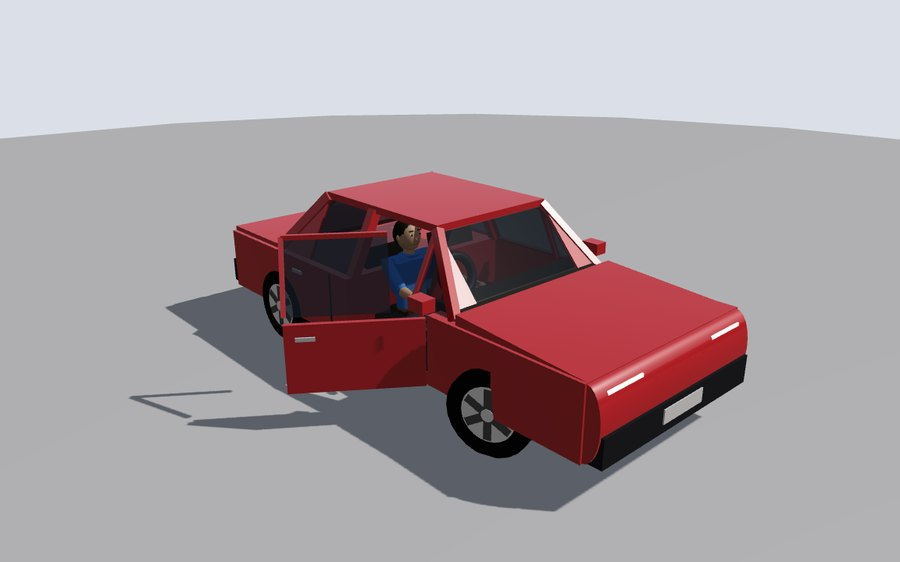
\includegraphics[width=\linewidth]{obj_car_red}\caption{Red}\end{subfigure}
\begin{subfigure}{0.32\linewidth}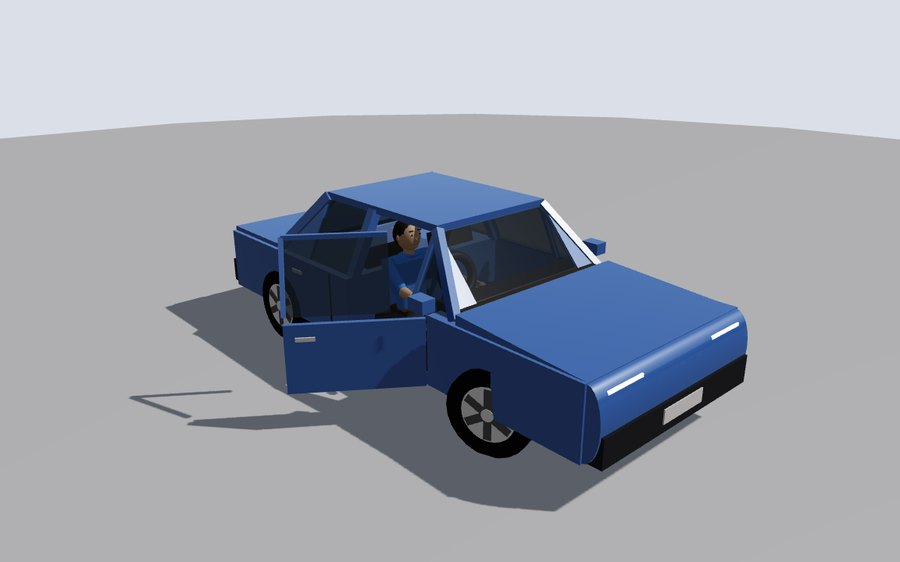
\includegraphics[width=\linewidth]{obj_car_blue}\caption{Blue}\end{subfigure}
\begin{subfigure}{0.32\linewidth}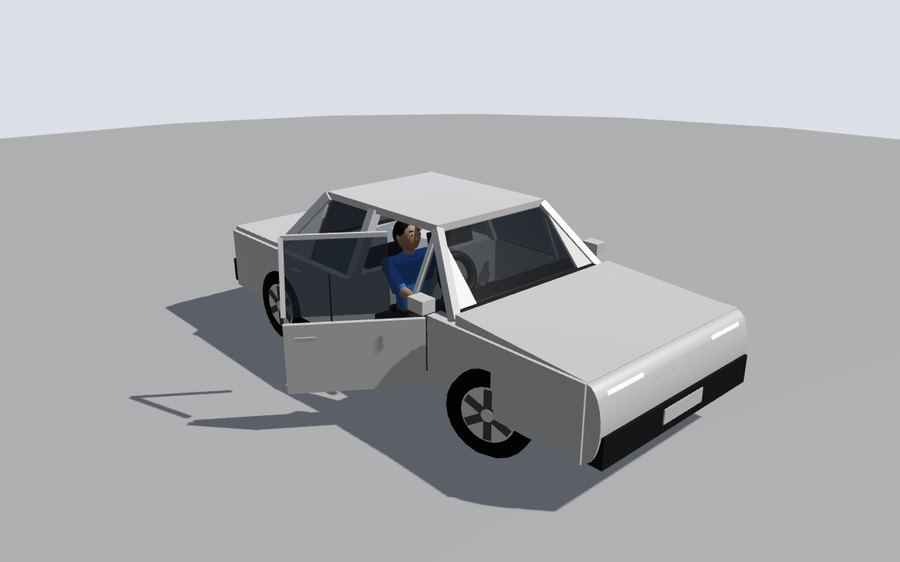
\includegraphics[width=\linewidth]{obj_car_white}\caption{White}\end{subfigure}
\caption{The car model in its three paint colours.}
\end{figure}
\objhead{Colours, textures and sound.} Glossy car paint, tinted transparent glass ($\alpha=0.45$), black rubber
tyres, polished metal rims and handles, glowing lights. Sounds: the door opening and closing when a visitor
gets in or out.

% =============================================================================
\subsection{Jungle}
% -----------------------------------------------------------------------------
\subsubsection{Rainforest tree}
\objviews{tree}{Rainforest tree: (a) complete, (b) disconnected parts.}
\objhead{Construction.} A low-poly trunk (6.5--9 m) and an upper trunk, four buttress roots (wedges), three
branches in nodes $R_y(yaw)\,R_x(45^\circ\ldots60^\circ)$, sometimes a hanging vine, and a crown: three dark core
blobs inside give the crown volume, and 15--19 alpha-tested leaf cards, each turned randomly about all three
axes, are placed on an ellipsoid shell around the crown centre $\mathbf{c}$:
\[
\mathbf{p} = \mathbf{c} + k\,(\cos\alpha\sqrt{1-y^2}\,r_x,\ y\,r_y,\ \sin\alpha\sqrt{1-y^2}\,r_z),\qquad
\alpha\in[0,2\pi),\ y\in[-0.55,1],\ k\in[0.55,1].
\]

\emph{Worked example: a buttress root.} Fin $i$ is a wedge with $S=(0.13,1.5,1.2)$ and $T=(0,0.75,0.6)$ inside a
node turned by $R_y(90^\circ i)$. For $i=1$: the bottom-front vertex $w_0=(-.5,-.5,.5)$ becomes $(-0.065,-0.75,0.6)$
after $S$, $(-0.065,0,1.2)$ after $T$, and $(1.2,\ 0,\ 0.065)$ after $R_y(90^\circ)$; the top-back vertex
$w_2=(-.5,.5,-.5)$ becomes $(0,\ 1.5,\ 0.065)$. Each fin therefore starts on the trunk 1.5 m above the ground and
reaches the ground 1.2 m away from it.
\objhead{Colours, textures and sound.} Bark texture, leaf-cluster cut-out texture, every card with a slightly
different green. Birds sing in the background by day (\Cref{sec:sound}).

% -----------------------------------------------------------------------------
\subsubsection{Coconut palm}
\objviews{palm}{Coconut palm: (a) complete, (b) disconnected parts.}
\objhead{Construction.} The trunk is a chain of seven segments. Each segment is a child of the previous one with
an extra $R_x(3^\circ\ldots7^\circ)$, so the rotations add up and the trunk bends smoothly:
$M_{k+1} = M_k\cdot T(0,L,0)\cdot R_x(\beta)$. Each segment has a ring. The crown has a heart (sphere), nine fronds made
of two quads (the outer half is a child of the inner half and droops by another $30^\circ\ldots45^\circ$) and four coconuts.
\objhead{Colours, textures and sound.} Bark texture, palm frond cut-out texture.

% -----------------------------------------------------------------------------
\subsubsection{Emergent tree}
\objviews{emergent}{Emergent giant tree: (a) complete, (b) disconnected parts.}
\objhead{Construction.} A 14--18 m trunk, five large buttress roots turned by $R_y(72^\circ\,i)$, four branches and
a wide, flat crown made of 20--24 leaf cards on a flattened ellipsoid ($r_x=r_z=4.2$, $r_y=1.3$). These trees
rise above the rest of the forest.
\objhead{Colours, textures and sound.} Light bark texture, leaf-cluster texture.

% -----------------------------------------------------------------------------
\subsubsection{Bamboo clump}
\objviews{bamboo}{Bamboo clump: (a) complete, (b) disconnected parts.}
\objhead{Construction.} 9--15 culms (thin low-poly cylinders) in nodes with a random position on a disc and a
small random tilt $R(\pm8^\circ,\ \text{random yaw},\ \pm8^\circ)$, node rings every 1.3 m and two leaf cards per culm.
\objhead{Colours, textures and sound.} Plain green culms, leaf-cluster texture.

% -----------------------------------------------------------------------------
\subsubsection{Banana plant}
\objviews{banana}{Banana plant: (a) complete, (b) disconnected parts.}
\objhead{Construction.} One to three pseudo-stems (cylinders); at the top of each, 5--8 long leaves are spheres
squashed to $(0.55,0.04,1.9)$ and turned by $R_y(360^\circ\,l/n)\,R_x(-35^\circ\ldots15^\circ)$. Some plants carry a
bunch of bananas on a stalk.
\objhead{Colours, textures and sound.} Matte greens; the leaves use two-sided foliage lighting.

% -----------------------------------------------------------------------------
\subsubsection{Undergrowth}
\objviews{undergrowth}{Undergrowth: a bush, a fern, a rock and a fallen log: (a) complete, (b) disconnected parts.}
\objhead{Construction.} A bush is a dark core sphere and 5--7 leaf cards (sometimes with flowers). A fern is
five quads tilted by $R_x(55^\circ)$ and turned by $R_y(72^\circ\,i)$ plus a cross card. A rock is 1--3 squashed
low spheres with random rotations. A fallen log is a horizontal cylinder ($R_z(90^\circ)$) with moss blobs and
mushrooms made of a cylinder stem and a hemisphere cap.
\objhead{Colours, textures and sound.} Leaf, fern, rock and bark textures.

% -----------------------------------------------------------------------------
\subsubsection{Bird}
\objviews[5.5cm]{bird}{Bird: (a) complete, (b) disconnected parts.}
\objhead{Construction.} A body (squashed sphere), a cone beak rotated $R_x(90^\circ)$ and two wings. Each wing is a
box in a child node rotated by $R_z(\pm\phi)$ about the body axis, with $\phi = 35^\circ\sin(\text{flap})$, so the two
wings flap symmetrically.
\objhead{Function.} Nine birds fly on circles above the jungle by day (\Cref{sec:effects}).

% -----------------------------------------------------------------------------
\subsubsection{Placement of the jungle, terrain and road}\label{sec:terrain}
The world ($280\times280$ m) is covered with a \emph{jittered grid} of 6.6 m cells. Each cell gets one random
point, and points inside the cleared area (building, lot and road with a margin) are skipped. A random number
then chooses the species: 40\% rainforest tree, 18\% palm, 7\% emergent tree, 8\% bamboo, 11\% banana, 8\% bush and
8\% nothing. Every cell also gets 1--5 ferns or bushes and 4--12 grass or flower tufts, a rock with 12\% and a log
with 5\% chance. In total the jungle has \statJungleTrees\ broad-leaf trees, \statPalms\ palms, \statBamboo\
bamboo clumps, \statBushes\ bushes, \statFerns\ ferns, \statGrass\ grass tufts, \statRocks\ rocks and
\statLogs\ logs. Every trunk gets a circle collider.

The terrain is flat in the clearing and along the road and becomes hilly further away:
\begin{align*}
H(x,z) &= 14\,\big(\mathrm{fbm}(0.018x,\,0.018z)-0.45\big) + 1.2\,\mathrm{fbm}(0.07x,\,0.07z) \\
h(x,z) &= \max\!\Big(-1.5,\ H(x,z)\cdot \mathrm{smoothstep}(0,30,d)\cdot \mathrm{smoothstep}\big(5,14,|z-z_{road}(x)|\big)\Big)
\end{align*}
where $d$ is the distance outside the clearing. The road is straight through the lot ($z=16$) and curves in the
jungle. With $t=|x|-30$,
\[
z_{road}(x)=16 + 7\sin(0.035\,t)\,\mathrm{sign}(x)\cdot \mathrm{smoothstep}(0,25,t).
\]
The smoothstep factor gives the bend a slope of zero at $t=0$, so the straight and the curved part join smoothly.
The road is built from 2 m boxes turned to follow the curve; neighbouring boxes overlap by 40 cm.

% =============================================================================
\section{Lighting and Shading}\label{sec:lighting}
\subsection{Illumination model}
The light leaving a surface point is computed with the \textbf{Phong illumination model} using Blinn's half
vector (the \emph{Blinn--Phong} model). It is the sum of three reflection terms:
\begin{table}[H]
\centering\small
\caption{The three terms of the illumination model}\label{tab:phongterms}
\begin{tabularx}{\linewidth}{@{}P{1.8cm}P{4.6cm}X@{}}
\toprule
Term & Formula & Meaning \\ \midrule
Ambient & $I_a\,k_a$ & light scattered by the whole scene; it reaches every surface, also in shadow \\
Diffuse & $I_l\,k_d\,\max(\mathbf{N}\cdot\mathbf{L},0)$ & Lambert's cosine law: the brightness depends on the angle between the surface and the light, not on the viewer \\
Specular & $I_l\,k_s\,\max(\mathbf{N}\cdot\mathbf{H},0)^{n}$ & the highlight; it moves with the viewer. A large shininess $n$ gives a small sharp highlight \\
\bottomrule
\end{tabularx}
\end{table}
Here $\mathbf{N}$ is the unit surface normal, $\mathbf{L}$ the unit vector towards the light, $\mathbf{V}$ the unit
vector towards the camera and $\mathbf{H}$ the half vector,
\[
\mathbf{H} = \frac{\mathbf{L}+\mathbf{V}}{|\mathbf{L}+\mathbf{V}|},\qquad
\mathbf{R} = 2(\mathbf{N}\cdot\mathbf{L})\,\mathbf{N}-\mathbf{L}.
\]
Phong's original specular term $(\mathbf{R}\cdot\mathbf{V})^n$ uses the mirror direction $\mathbf{R}$; the half-vector
form $(\mathbf{N}\cdot\mathbf{H})^n$ gives nearly the same highlight and is cheaper to compute. For one light the model is
\[
I = I_a k_a + I_l\big(k_d\max(\mathbf{N}\!\cdot\!\mathbf{L},0) + k_s\max(\mathbf{N}\!\cdot\!\mathbf{H},0)^{n}\big).
\]
The fragment shader evaluates this sum over all active lights:
\[
C = \underbrace{\text{mix}\!\big(A_{ground},A_{sky},\tfrac{N_y+1}{2}\big)\,k_d}_{\text{ambient}}
 + \sum_{lights}\Big(k_d\max(\mathbf{N}\!\cdot\!\mathbf{L},0) + k_s\max(\mathbf{N}\!\cdot\!\mathbf{H},0)^{n}\Big)\,I\,a(d)\,c\,s
 + E .
\]
$k_d$ is the surface colour multiplied by the texture, $k_s$ the specular strength, $n$ the shininess, $I$ the
light colour times its intensity, $a(d)$ the distance attenuation, $c$ the spot-light cone factor, $s$ the shadow
factor (\Cref{sec:shadows}) and $E$ the emission of glowing surfaces. The ambient term is a \emph{hemisphere} light:
surfaces facing up receive the sky colour and surfaces facing down the ground colour. Inside the building it is
multiplied by 0.45, because the roof blocks the sky. Point and spot lights fade smoothly to zero at their
range $r$:
\[
a(d) = \frac{\big[\mathrm{clamp}(1-(d/r)^4,\,0,\,1)\big]^2}{1+d^2},\qquad
c = \mathrm{smoothstep}\big(\cos\theta_{out},\ \cos\theta_{in},\ -\mathbf{L}\cdot\mathbf{D}\big),
\]
where $\mathbf{D}$ is the spot direction and $\theta_{in}$, $\theta_{out}$ are its inner and outer cone angles.

\paragraph{Materials.} Every material carries its own $k_s$ and $n$ (\Cref{tab:materials}). Leaves and grass
use \emph{wrap} lighting, $0.6\,\mathbf{N}\!\cdot\!\mathbf{L}+0.4$, are lit from both sides, and gain a translucency term
$0.45\,k_d\,I\,s\,\max(-\mathbf{V}\cdot\mathbf{L},0)^3$ when the sun is behind them. Polished metal (bins, door
handles, wheel rims) uses a weak diffuse part $0.25\,k_d$ and a highlight in the colour of the metal, $3k_d$; it
also reflects a simple painted surrounding $E_{env}(\mathbf{R}_v)$ (sky, horizon and ground) in the mirror direction
$\mathbf{R}_v=2(\mathbf{N}\cdot\mathbf{V})\mathbf{N}-\mathbf{V}$. Car paint adds a clear-coat reflection weighted with
Schlick's approximation $F=(1-\mathbf{N}\cdot\mathbf{V})^5$:
\[
C_{metal} = C(0.25\,k_d,\ 3k_d) + E_{env}(\mathbf{R}_v)\,k_d\,(0.85+0.15F),\qquad
C_{paint} = C(k_d,\ 2.5) + E_{env}(\mathbf{R}_v)\,(0.08+0.75F).
\]
\begin{table}[H]
\centering\small
\caption{Typical material parameters}\label{tab:materials}
\begin{tabular}{@{}lcc l@{}}
\toprule
Material & $k_s$ & $n$ & Used for \\ \midrule
Fabric, plaster, bark, brick, matte & 0.03--0.05 & 6--8 & sofas, walls, trees, soil \\
Rubber & 0.08 & 8 & tyres \\
Wood, leather & 0.2--0.3 & 24 & furniture, shelves \\
Plastic, painted metal, steel & 0.35--0.6 & 48--64 & machines, keys, lamps \\
Marble & 0.6 & 96 & counter top, window sills \\
Glass & 1.0 & 160 & windows, front glass, aquarium \\
Car paint & 1.0 & 160 & cars (with clear-coat reflection) \\
Polished metal & 1.0 & 200 & bins, handles, rims (with reflection) \\
\bottomrule
\end{tabular}
\end{table}

\subsection{Light sources in the scene}
\begin{table}[H]
\centering\small
\caption{Light types used in the scene and the figures in which they can be seen}\label{tab:lighttypes}
\begin{tabularx}{\linewidth}{@{}P{1.8cm}P{3.4cm}XP{2.7cm}@{}}
\toprule
Type & Behaviour & Where in the scene & Figures \\ \midrule
Directional & same direction $\mathbf{L}$ everywhere, no attenuation & the \textbf{sun} by day and the \textbf{moon} by night & \Cref{fig:daytimes} \\
Point & radiates in all directions from a position, attenuated by $a(d)$ & lounge pendants (4), library pendants (3), ATM tube lights (2), vending machine interiors (3), ATM screen, aquarium hood, TV glow, street lamps & \Cref{fig:lampsonoff}, \Cref{fig:nightlights}, \Cref{fig:visitors} \\
Spot & a point light limited to a cone & downlights over the vending machines, the TV wall and the coffee counter, the reading lamp, porch lights, car headlights & \Cref{fig:vendbuy}, \Cref{fig:nightlights} \\
Emissive & the surface glows by itself and lights nothing else & bulbs, tubes, LEDs, screens, signs, fireflies & \Cref{fig:lampsonoff}, \Cref{fig:split_pendant} \\
Ambient & sky colour from above, ground colour from below & everywhere, changes with the time of day & \Cref{fig:lampsonoff}(b) \\
\bottomrule
\end{tabularx}
\end{table}
Every light belongs to a \emph{group}: lounge, spots, ATM room, library, outdoor or machines. Groups are switched
with the F1--F4 keys or with the light switches on the walls, and the lamp models check their group, so a bulb only
glows when its light is on. The outdoor group switches on automatically at dusk.

\begin{figure}[H]
\centering
\begin{subfigure}{0.49\linewidth}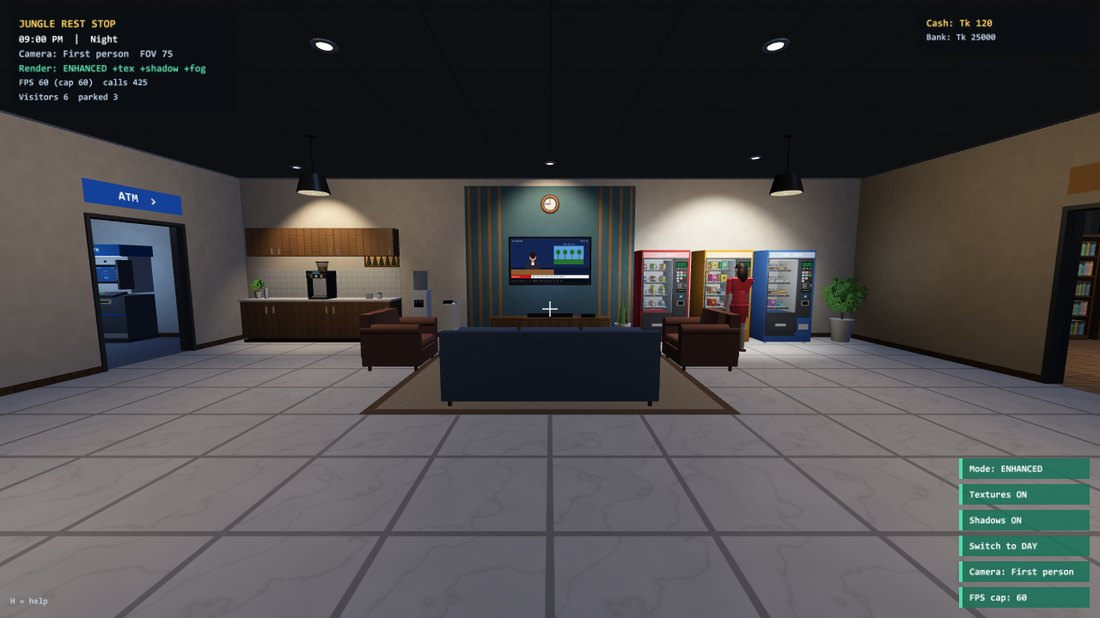
\includegraphics[width=\linewidth]{lounge_night}\caption{Night, lamps on}\end{subfigure}
\begin{subfigure}{0.49\linewidth}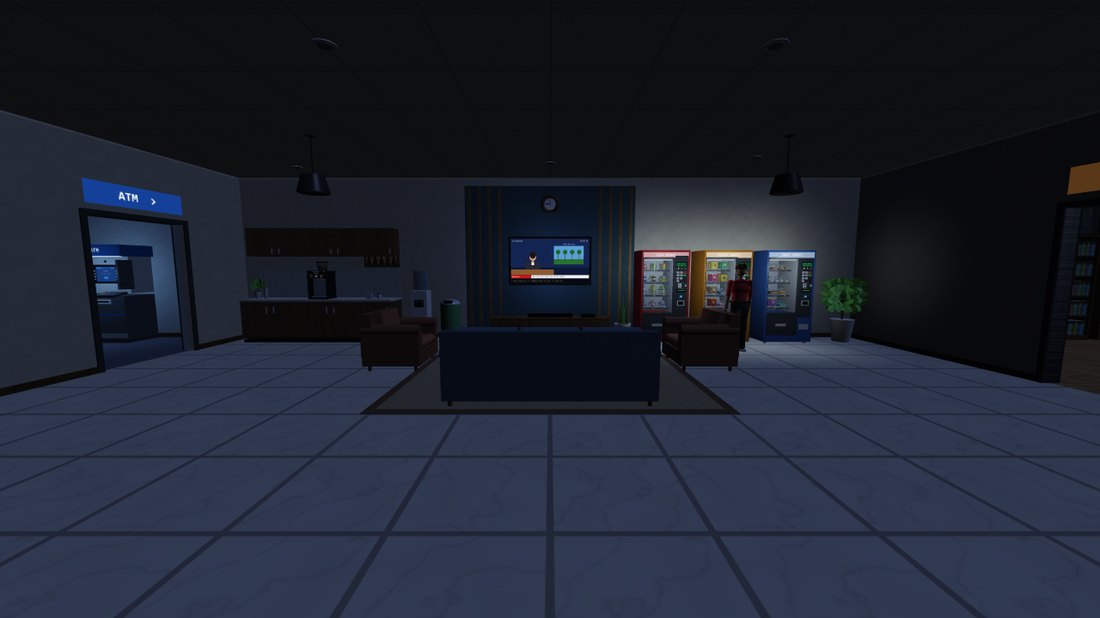
\includegraphics[width=\linewidth]{lounge_night_lamps_off}\caption{Night, lamps off (machine glow and moonlight)}\end{subfigure}
\caption{The lounge with and without its point and spot lights.}\label{fig:lampsonoff}
\end{figure}
\begin{figure}[H]
\centering
\begin{subfigure}{0.49\linewidth}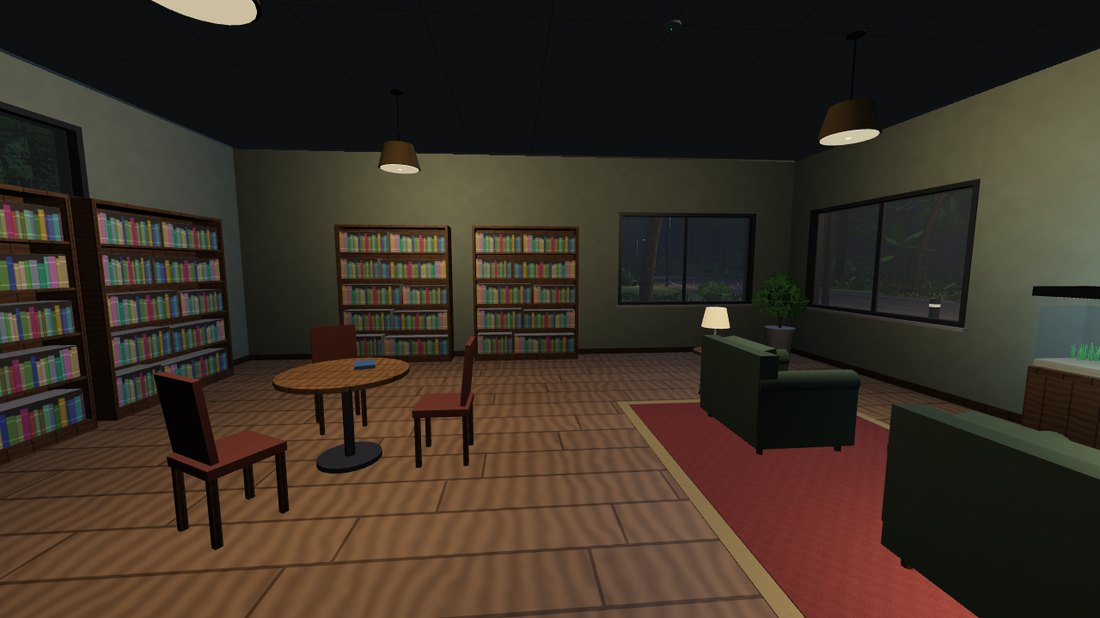
\includegraphics[width=\linewidth]{library_night}\caption{Library at night: pendants and reading lamp}\end{subfigure}
\begin{subfigure}{0.49\linewidth}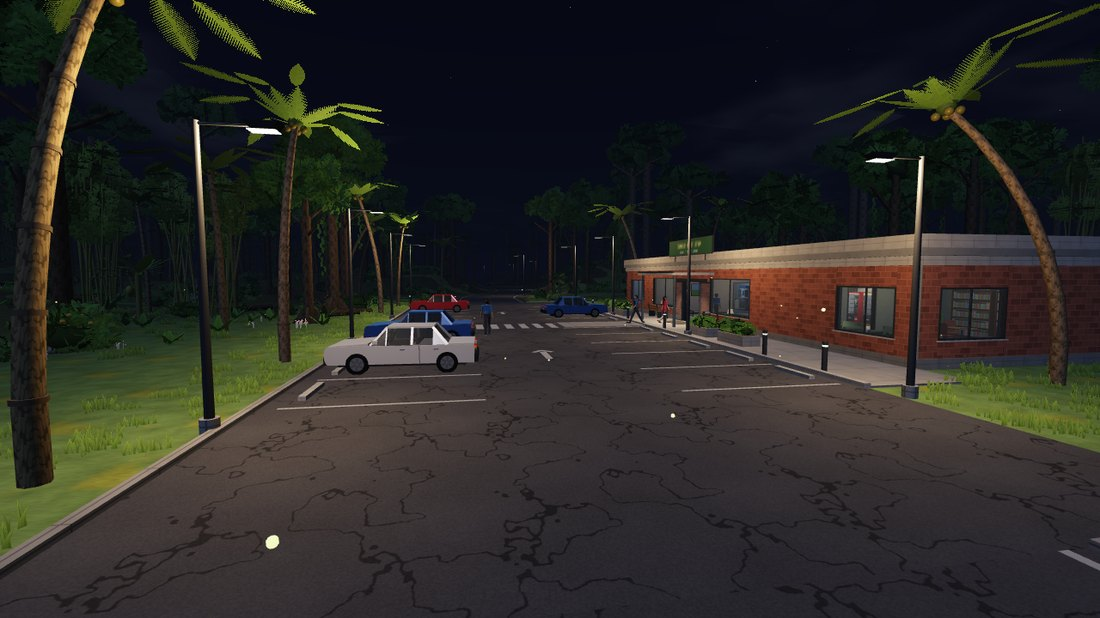
\includegraphics[width=\linewidth]{parking_night}\caption{Street lamps and car lights}\end{subfigure}
\caption{Point, spot and emissive lights at night.}\label{fig:nightlights}
\end{figure}

\subsection{Per-frame light selection}
The shader accepts up to 32 point lights and 16 spot lights. Every frame the light manager
\begin{enumerate}
  \item removes lights that are switched off or whose sphere of influence
        lies outside the view frustum,
  \item keeps the nearest ones, and
  \item sorts them by \textbf{region}: ATM room, lounge, library or outdoors.
\end{enumerate}
Each pixel determines its region from its position and loops only over the lights of that region. Light
therefore never passes through a wall into the next room, and each pixel evaluates fewer lights.

% -----------------------------------------------------------------------------
\subsection{Shading method}\label{sec:shading}
The scene uses \textbf{Phong shading}: the illumination model is evaluated once per pixel with an interpolated
normal (\Cref{fig:shadingpipe}).
\begin{figure}[H]
\centering
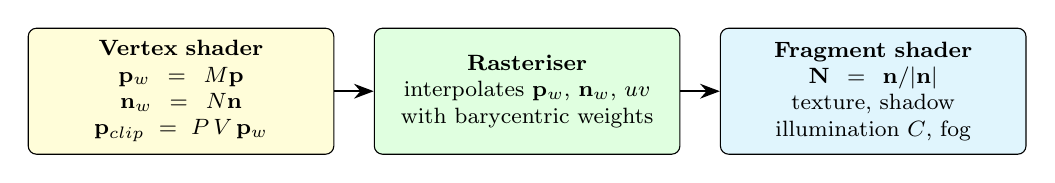
\begin{tikzpicture}[node distance=0.5cm,b/.style={box,text width=3.6cm,minimum height=1.6cm,font=\footnotesize}]
\node[b,fill=yellow!15] (vs) {\textbf{Vertex shader}\\$\mathbf{p}_w = M\mathbf{p}$\\$\mathbf{n}_w = N\mathbf{n}$\\$\mathbf{p}_{clip}=P\,V\,\mathbf{p}_w$};
\node[b,fill=green!12,right=of vs] (ra) {\textbf{Rasteriser}\\interpolates $\mathbf{p}_w$, $\mathbf{n}_w$, $uv$ with barycentric weights};
\node[b,fill=cyan!12,right=of ra] (fs) {\textbf{Fragment shader}\\$\mathbf{N}=\mathbf{n}/|\mathbf{n}|$\\texture, shadow\\illumination $C$, fog};
\draw[arr] (vs)--(ra); \draw[arr] (ra)--(fs);
\end{tikzpicture}
\caption{Phong shading in the OpenGL pipeline.}\label{fig:shadingpipe}
\end{figure}
\begin{enumerate}
  \item The vertex shader transforms the position into world space and the normal with the normal matrix
        $N=(M^{-1})^T$, and sends both to the rasteriser.
  \item For a pixel inside a triangle with vertices $\mathbf{p}_0,\mathbf{p}_1,\mathbf{p}_2$, the rasteriser computes the
        barycentric weights $(\alpha,\beta,\gamma)$, $\alpha+\beta+\gamma=1$, and interpolates every value
        (perspective-correct):
        \[
        \mathbf{n}(\alpha,\beta,\gamma) = \alpha\,\mathbf{n}_0 + \beta\,\mathbf{n}_1 + \gamma\,\mathbf{n}_2,\qquad
        \mathbf{p}(\alpha,\beta,\gamma) = \alpha\,\mathbf{p}_0 + \beta\,\mathbf{p}_1 + \gamma\,\mathbf{p}_2 .
        \]
  \item The interpolated normal is shorter than 1 inside the triangle, so the fragment shader normalises it,
        $\mathbf{N}=\mathbf{n}/|\mathbf{n}|$, computes $\mathbf{L}$, $\mathbf{V}=\operatorname{normalize}(\mathbf{e}-\mathbf{p})$ and
        $\mathbf{H}$, and evaluates the illumination model $C$ of the previous section for this pixel.
\end{enumerate}
Whether a surface looks smooth or faceted is decided by its vertex normals. A cube stores separate vertices for
every face with the face normal, so all pixels of a face get the same normal and the edges are sharp. A sphere or
a cylinder stores one outward normal per vertex, so the interpolated normal changes smoothly across a triangle
and the surface looks round even with 20 or 24 sides (compare the shapes in \Cref{tab:shapes}). Because the
specular term is evaluated per pixel, highlights stay sharp in the middle of large triangles, for example on
the floor tiles and on the car bonnet. The same shading is used in Basic mode, without textures, shadows and fog.

% =============================================================================
\section{Day and Night}
A 24-hour clock runs at one game hour per 20 s (keys change the speed, pause it or jump between day and
night). The sun direction is computed from the hour:
\[
a=\frac{hour-6}{12}\pi,\qquad \mathbf{s}=\operatorname{normalize}(0.95\cos a,\ \sin a,\ 0.42),\qquad
\mathbf{m} = \operatorname{normalize}(-0.8\,s_x,\ -s_y,\ 0.3).
\]
The sun rises in the east ($+x$) at 6:00, is highest at noon and sets at 18:00; the moon $\mathbf{m}$ is on the
opposite side. All other values are blended from the sun height $s_y$: the sky zenith and horizon colours (with an
orange glow near sunrise and sunset), the sun colour, the ambient light, the fog colour and density, the cloud
colour and the exposure. The night factor
\[
\nu = 1-\mathrm{smoothstep}(-0.14,\,0.10,\,s_y)
\]
shows the stars and the moon, switches on the street lamps and the car headlights and wakes up the fireflies.
\Cref{fig:daytimes} shows the same view at four times of day.

% =============================================================================
\section{Textures}
\subsection{Procedural textures}
All 25 textures are generated at start-up from \emph{value noise}: random values on a grid are smoothly
interpolated, and several octaves are added (fractal Brownian motion):
\[
\mathrm{fbm}(\mathbf{p}) = \frac{\sum_{i=0}^{k-1} 0.5^{i}\,\mathrm{noise}(2^{i}\mathbf{p})}{\sum_{i=0}^{k-1}0.5^{i}} .
\]
The noise wraps around at the texture border, so the textures tile without seams. Patterns are built on top of it:
rows of bricks with mortar, wooden planks with grain $\sin(6v+\text{noise})$, tiles with grout, marble veins, woven
fabric, bark ridges, and \emph{cut-out} textures (leaves, grass, fern, palm frond, flowers, vine) whose alpha
channel marks the shape of the leaf.
\begin{figure}[H]\centering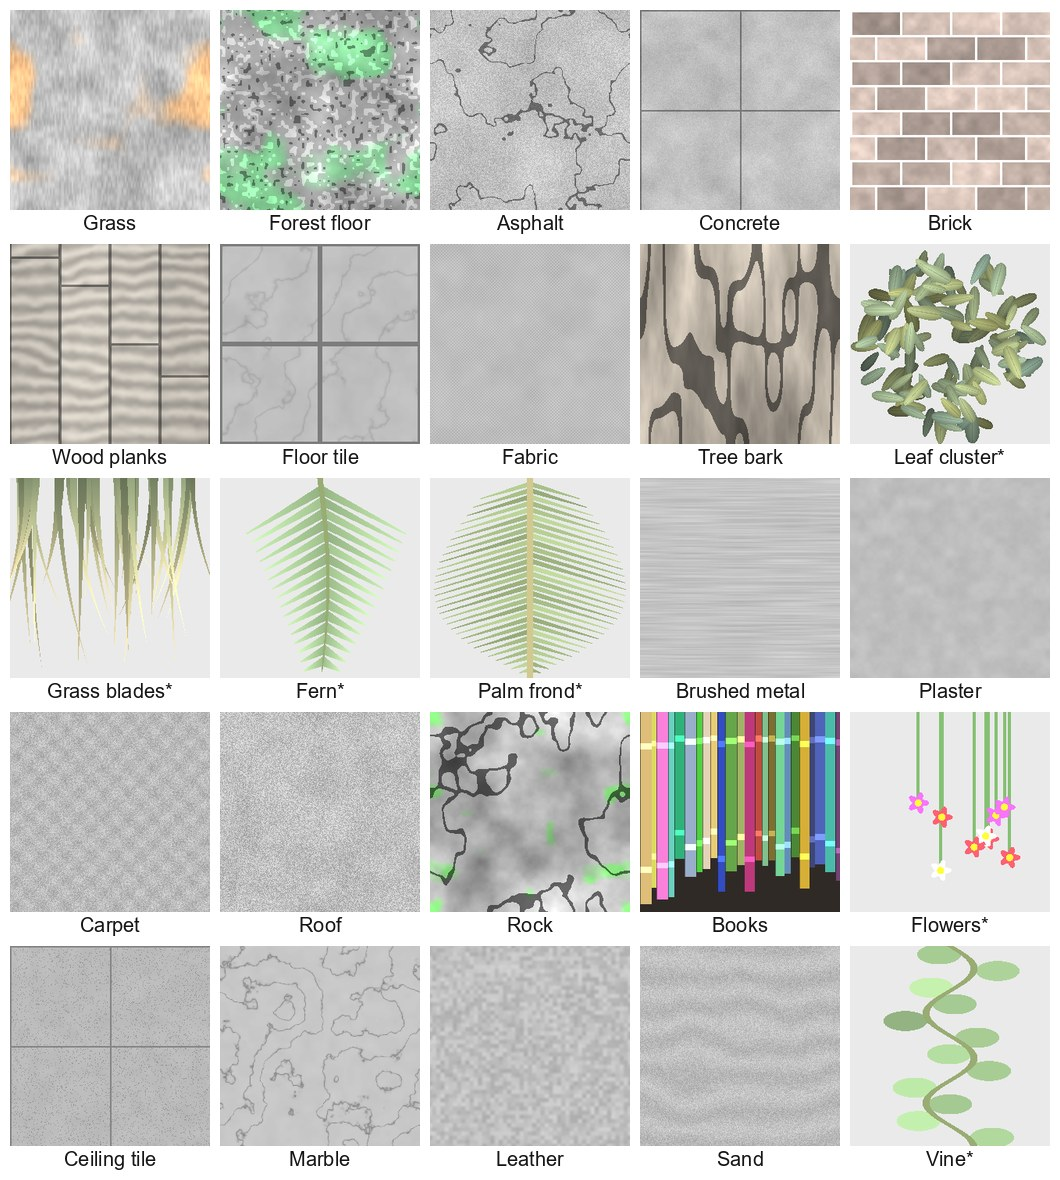
\includegraphics[width=0.9\linewidth]{textures}\caption{All procedural textures ($*$ = cut-out; light grey marks the transparent part).}\end{figure}

\subsection{Texture mapping}
\begin{itemize}
  \item All textures are layers of one \texttt{GL\_TEXTURE\_2D\_ARRAY} ($256\times256$, mip-maps, $4\times$
        anisotropic filtering). An instance only stores a layer number, so a texture change never breaks an
        instanced draw call.
  \item A texture stores a \emph{detail} value, and the final colour is $k_d = \text{colour}\times 2\cdot\text{texel}$,
        so the same brick texture works for any brick colour.
  \item \textbf{Object-space box mapping}: the shader selects the plane of the largest component of the local
        normal $\mathbf{n}_\ell$ and multiplies the local position $\mathbf{p}_\ell$ by the object's scale and the number of
        repeats per metre $\rho$:
        \[
        (u,v) = \rho\cdot\begin{cases}(x_\ell,\ z_\ell) & |n_y|\ge|n_x|,|n_z|\\ (z_\ell,\ y_\ell) & |n_x|\ge|n_z|\\ (x_\ell,\ y_\ell) & \text{otherwise}\end{cases}
        \]
        A 10 m wall therefore shows ten times more bricks than a 1 m box, without texture coordinates in the mesh.
  \item Cut-out cards use their mesh texture coordinates, and pixels with $\alpha<0.5$ are discarded, also in the
        shadow pass, so leaves cast leaf-shaped shadows.
  \item The terrain blends lawn grass and forest floor with a large-scale noise and the distance from the clearing.
\end{itemize}

% =============================================================================
\section{Shadows}\label{sec:shadows}
Shadows use \textbf{shadow mapping} (\Cref{fig:shadowidea}).
\begin{enumerate}
  \item \textbf{Depth pass}: the scene is drawn from the sun with an orthographic camera ($\pm32$ m around the
        player, a $2048\times2048$ depth texture, about 3 cm per texel). Only the depth is stored.
  \item \textbf{Main pass}: every pixel is transformed into the light's space with a small offset along its normal,
        \[
        \mathbf{p}_{L} = P_L\,V_L\,(\mathbf{p}+0.05\,\mathbf{N}),\qquad (u,v,z) = \tfrac12\,\mathbf{p}_L/w_L + \tfrac12,
        \]
        and compared with the stored depth $z_{map}(u,v)$: the pixel is lit if $z - b \le z_{map}$, with the
        slope-scaled bias $b = 0.0006+0.0012(1-\mathbf{N}\cdot\mathbf{L})$.
  \item \textbf{Percentage-closer filtering}: five hardware-compared samples around $(u,v)$ (the centre counted twice)
        are averaged, $s=\frac16\sum_k w_k\,[z-b\le z_{map}(u_k,v_k)]$, which gives soft shadow edges.
\end{enumerate}
The shadow camera moves only in whole texels along its own axes and the light direction used for shadows changes
in steps of $0.5^\circ$, so shadow edges do not shimmer when the camera or the sun moves. Glass, grass and other
small details do not cast shadows.
\begin{figure}[H]
\centering
\begin{minipage}{0.42\linewidth}
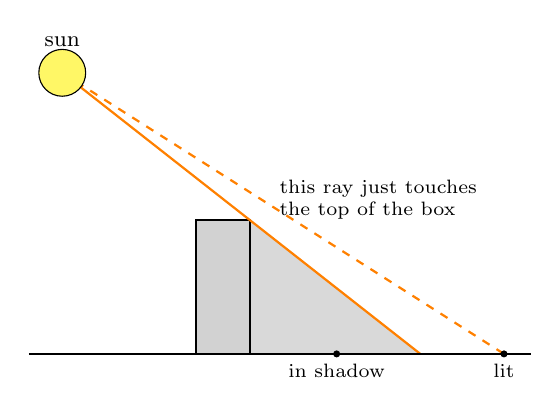
\begin{tikzpicture}[scale=0.85]
\fill[black!15] (2.8,0) -- (5.35,0) -- (2.8,2) -- cycle;
\draw[thick,fill=gray!35] (2,0) rectangle (2.8,2);
\draw[orange,thick] (0,4.2) -- (5.35,0);
\draw[orange,thick,dashed] (0,4.2) -- (6.6,0);
\draw[fill=yellow!60] (0,4.2) circle (0.35) node[above=6pt,font=\footnotesize]{sun};
\draw[thick] (-0.5,0) -- (7,0);
\fill (4.1,0) circle (1.5pt) node[below,font=\scriptsize]{in shadow};
\fill (6.6,0) circle (1.5pt) node[below,font=\scriptsize]{lit};
\node[font=\scriptsize,align=left,anchor=west] at (3.1,2.3) {this ray just touches\\the top of the box};
\end{tikzpicture}
\end{minipage}
\begin{minipage}{0.4\linewidth}
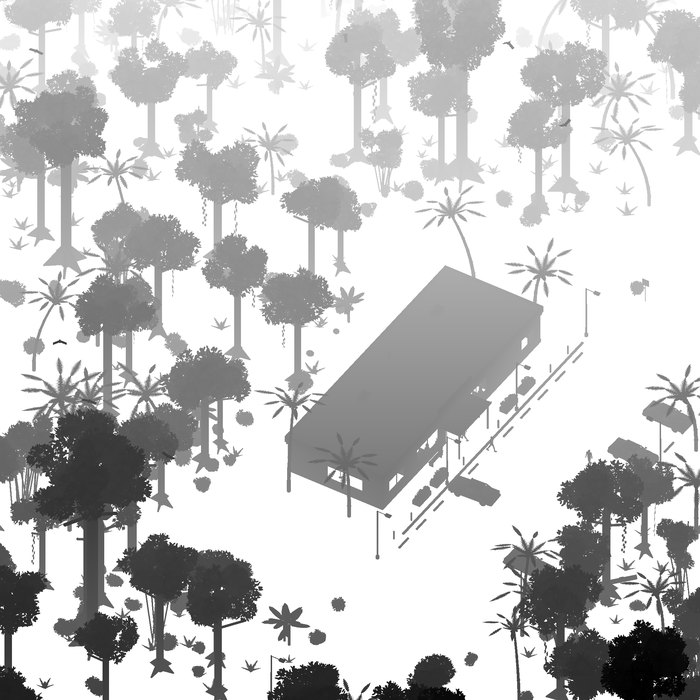
\includegraphics[width=\linewidth]{shadow_map}
\end{minipage}
\caption{Left: the principle of shadow mapping. Right: the depth image seen by the sun (darker = closer).}\label{fig:shadowidea}
\end{figure}
\begin{figure}[H]
\centering
\begin{subfigure}{0.49\linewidth}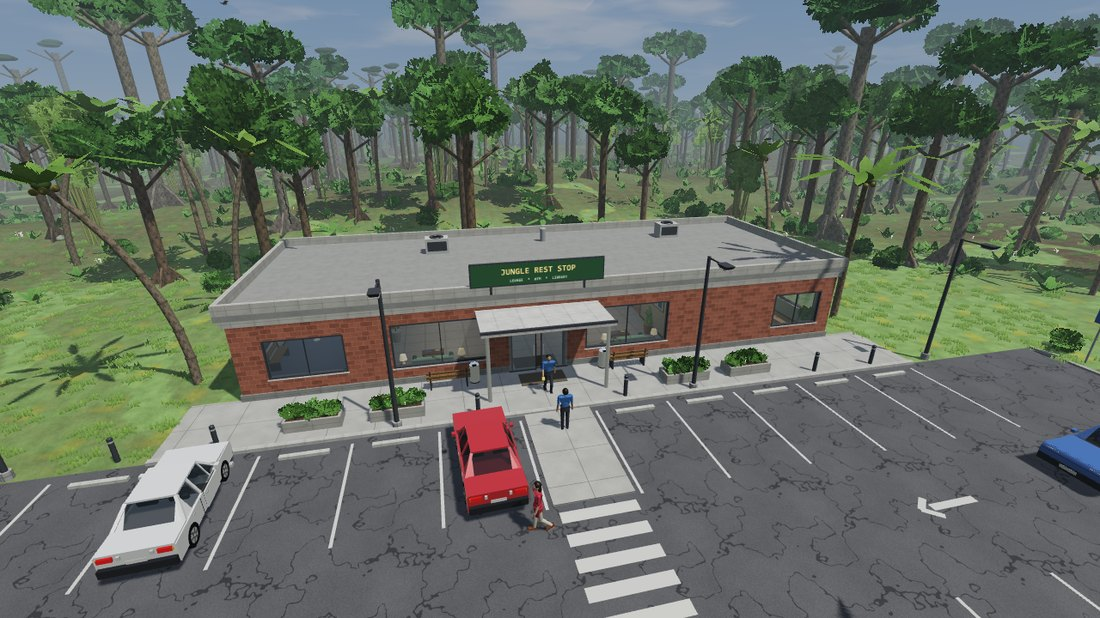
\includegraphics[width=\linewidth]{ext_day}\caption{Shadows on}\end{subfigure}
\begin{subfigure}{0.49\linewidth}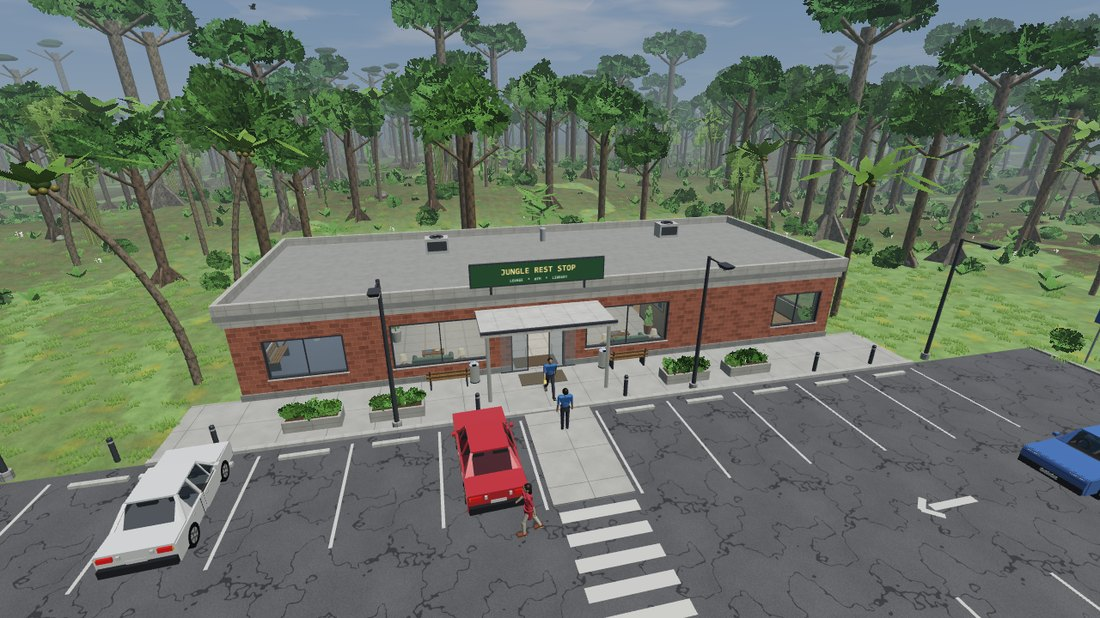
\includegraphics[width=\linewidth]{ext_day_noshadow}\caption{Shadows off}\end{subfigure}
\caption{Shadows show where objects touch the ground and give the scene depth.}
\end{figure}

% =============================================================================
\section{Sky, Fog, Tone Mapping and Wind}\label{sec:sky}
\begin{itemize}
  \item \textbf{Sky}: one full-screen triangle. For each pixel the view ray $\mathbf{d}$ is rebuilt with the inverse
        view-projection matrix. The colour is $\text{mix}(horizon, zenith, h^{0.55})$ ($h$ = height of the ray), plus a
        sun disc $\max(\mathbf{d}\cdot\mathbf{s},0)^{900}$ with a glow, a moon, twinkling stars (a hash on a 3D grid)
        and moving clouds (4-octave noise projected on a sky plane).
  \item \textbf{Fog}: the colour is blended towards the horizon colour with
        \[
        f = 1-e^{-(d\rho)^{1.5}},\qquad C' = (1-f)\,C + f\,C_{fog},
        \]
        where $d$ is the distance and $\rho$ the density. It hides the end of the world and gives a humid look; it is
        denser at night and thinner when the camera is high up.
  \item \textbf{Tone mapping}: $C' = 1-e^{-C\cdot exposure}$ keeps bright lamps from turning flat white. The exposure
        rises at night.
  \item \textbf{Wind}: leaves and grass sway in the vertex shader. The offset grows with the height inside the shape:
        $\Delta x = 0.05\,h\,\min(s_y,2.5)\sin(1.7t+0.35x+0.27z)$. The aquarium plants use the same rule as a water current.
\end{itemize}

% =============================================================================
\section{Basic Mode and Enhanced Mode}
\textbf{B} (or the on-screen button) switches between the modes; \textbf{T}, \textbf{G} and \textbf{F} switch
textures, shadows and fog one at a time.
\begin{table}[H]
\centering\small
\begin{tabular}{@{}lcc@{}}
\toprule
Feature & Basic & Enhanced \\ \midrule
Basic shapes, transformations, all objects & yes & yes \\
Blinn--Phong lighting with all lights, Phong shading & yes & yes \\
Procedural textures & -- & yes \\
Shadow mapping (PCF) & -- & yes \\
Fog & -- & yes \\
Sky with sun, clouds, stars & gradient & yes \\
Wind animation & -- & yes \\
Tone mapping & clamp & exponential \\
\bottomrule
\end{tabular}
\end{table}
\begin{figure}[H]
\centering
\begin{subfigure}{0.49\linewidth}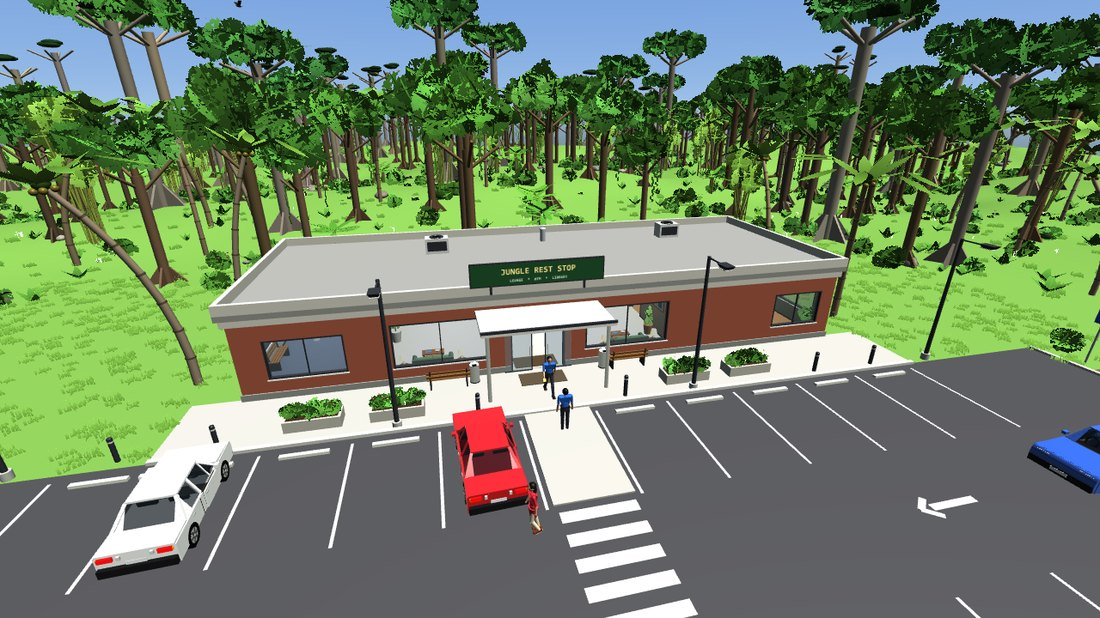
\includegraphics[width=\linewidth]{ext_day_basic}\caption{Basic}\end{subfigure}
\begin{subfigure}{0.49\linewidth}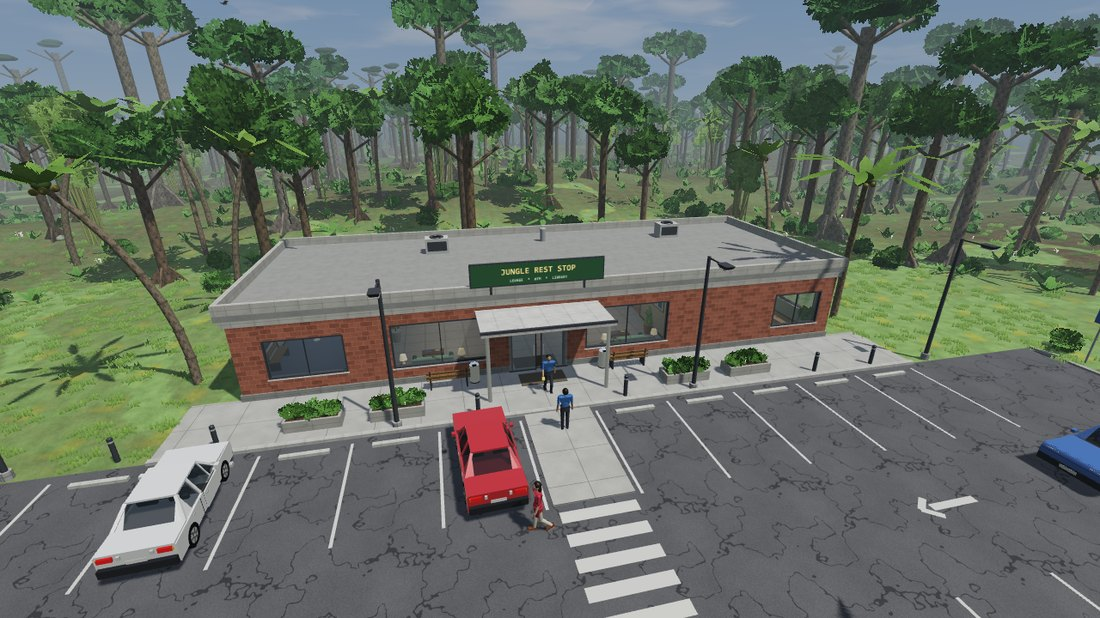
\includegraphics[width=\linewidth]{ext_day}\caption{Enhanced}\end{subfigure}
\begin{subfigure}{0.49\linewidth}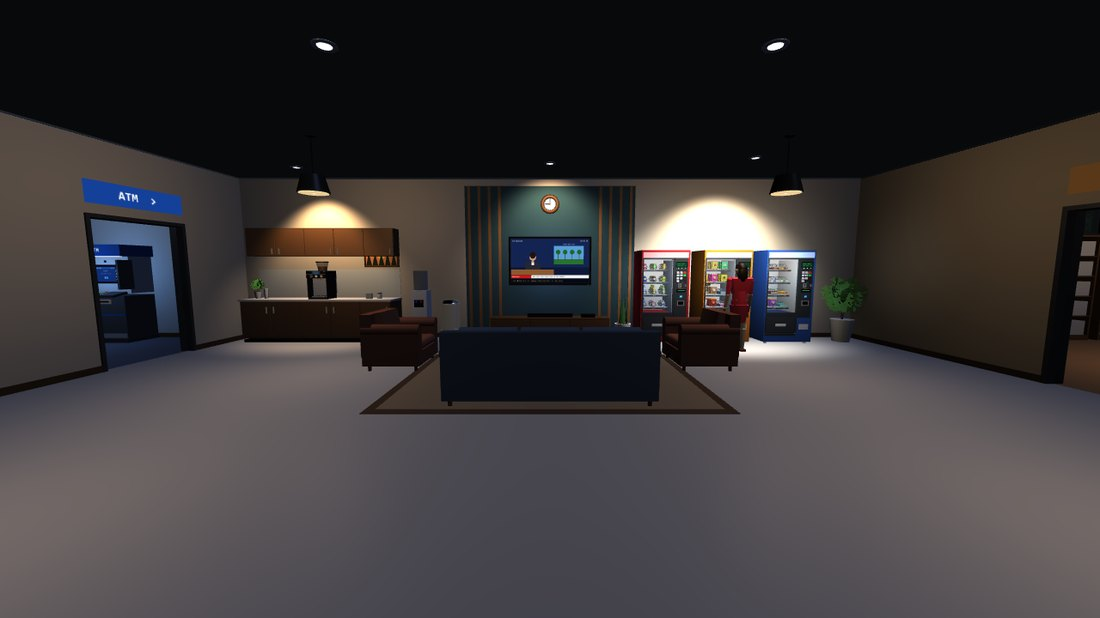
\includegraphics[width=\linewidth]{lounge_night_basic}\caption{Basic (interior)}\end{subfigure}
\begin{subfigure}{0.49\linewidth}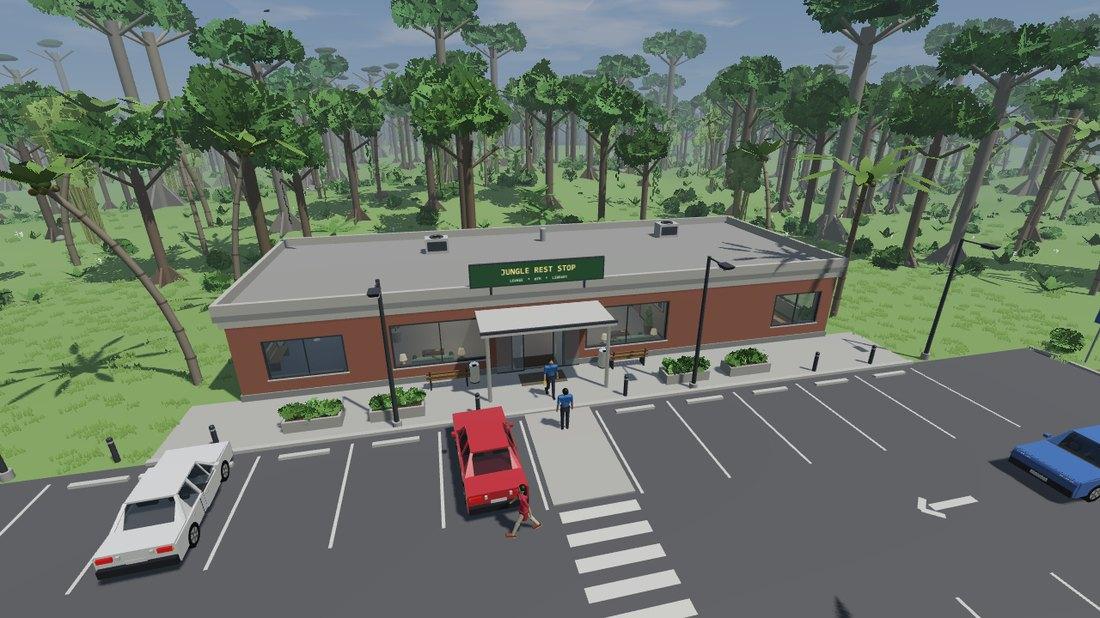
\includegraphics[width=\linewidth]{ext_day_notex}\caption{Enhanced without textures}\end{subfigure}
\caption{Basic and Enhanced rendering.}
\end{figure}

% =============================================================================
\section{The Player and Interaction}\label{sec:interaction}
The user controls a person (the man model of \Cref{sec:humans}) who walks through the scene and operates the
machines by looking at a part and pressing \textbf{E} or the left mouse button. This section explains how the
player moves, how the program finds the part that is looked at, and how every object reacts.

\subsection{Movement of the player}\label{sec:camera}
\paragraph{Walking.} The player has a position $\mathbf{p}$ (the feet), a yaw angle $\psi$ (turning left and right)
and a pitch angle $\theta$ (looking up and down). Moving the mouse by $(\Delta m_x,\Delta m_y)$ pixels changes
\[
\psi \leftarrow \psi - 0.12\,\Delta m_x,\qquad \theta \leftarrow \mathrm{clamp}(\theta - 0.12\,\Delta m_y,\ -85^\circ,\ 85^\circ).
\]
The keys W, S, A, D give a forward input $w\in\{-1,0,1\}$ and a sideways input $a\in\{-1,0,1\}$. The forward and the
right direction on the ground follow the yaw:
\[
\mathbf{f} = (\sin\psi,\ 0,\ \cos\psi),\qquad \mathbf{r} = (-\cos\psi,\ 0,\ \sin\psi),\qquad
\mathbf{p} \leftarrow \mathbf{p} + \operatorname{normalize}(w\,\mathbf{f} + a\,\mathbf{r})\; v\,\Delta t,
\]
with the speed $v=2.4$ m/s (walking) or $5.0$ m/s (Shift, running). Gravity and jumping act on the height:
$v_y \leftarrow v_y - 12\,\Delta t$, $p_y \leftarrow p_y + v_y\Delta t$, and $p_y$ never goes below the terrain height; Space
sets $v_y=4.6$ m/s. While walking, the walk phase grows by $7\,\Delta t$ and drives the body animation of
\Cref{sec:humans} and a small head bob $0.028\sin(2\varphi)$ of the first-person camera.

\paragraph{Collision.} The player is a circle of radius $r=0.3$ m on the ground. Walls, machines, furniture and cars are
oriented boxes with a height range; tree trunks, posts and people are circles. To push the player out of a box, the
centre is moved into the box's own frame (rotation by $-yaw_{box}$), the nearest point of the box is found by clamping,
\[
\mathbf{q}=\mathrm{clamp}(\mathbf{p}_{local},\,-\mathbf{h},\,\mathbf{h}),\qquad
\text{if } |\mathbf{p}_{local}-\mathbf{q}|<r:\quad \mathbf{p}_{local} \leftarrow \mathbf{q} + r\,\frac{\mathbf{p}_{local}-\mathbf{q}}{|\mathbf{p}_{local}-\mathbf{q}|},
\]
and the result is turned back. Two circles are separated in the same way along the line between their centres.
The test is repeated three times per frame so corners work, and a box only counts when it overlaps the player's
height, so the player can walk under a table top. The sliding doors switch their box off while they are open.

\paragraph{Cameras.} Key V cycles through three cameras (\Cref{fig:cameras}):
\begin{itemize}
  \item \textbf{First person}: the camera is at eye height and looks along the view direction:
        \[\mathbf{e}=\mathbf{p}+(0,\,1.62,\,0),\qquad \mathbf{d}=(\sin\psi\cos\theta,\ \sin\theta,\ \cos\psi\cos\theta).\]
  \item \textbf{Third person}: the body is visible; the camera is placed $3.4$ m behind the head along $-\mathbf{d}$ and
        $0.35$ m higher. A ray from the head to the camera is tested against the collision boxes and the camera moves
        closer when a wall is in the way.
  \item \textbf{Free camera}: flies without collision (W A S D, Space, Ctrl) to inspect the scene, for example with
        the roof cut-away view.
\end{itemize}
The mouse wheel changes the field of view $f$ between $25^\circ$ and $110^\circ$, which changes the $1/\tan(f/2)$ terms of
the projection matrix (\Cref{sec:transform}).
\begin{figure}[H]
\centering
\begin{subfigure}{0.49\linewidth}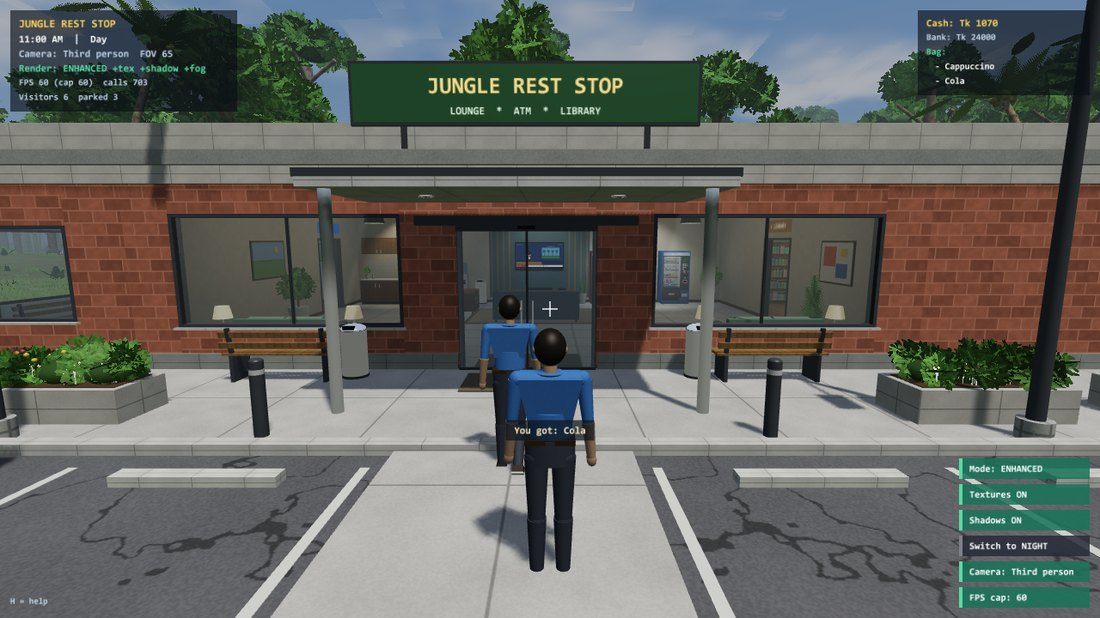
\includegraphics[width=\linewidth]{play_walk_1}\caption{Third person: walking to the entrance}\end{subfigure}
\begin{subfigure}{0.49\linewidth}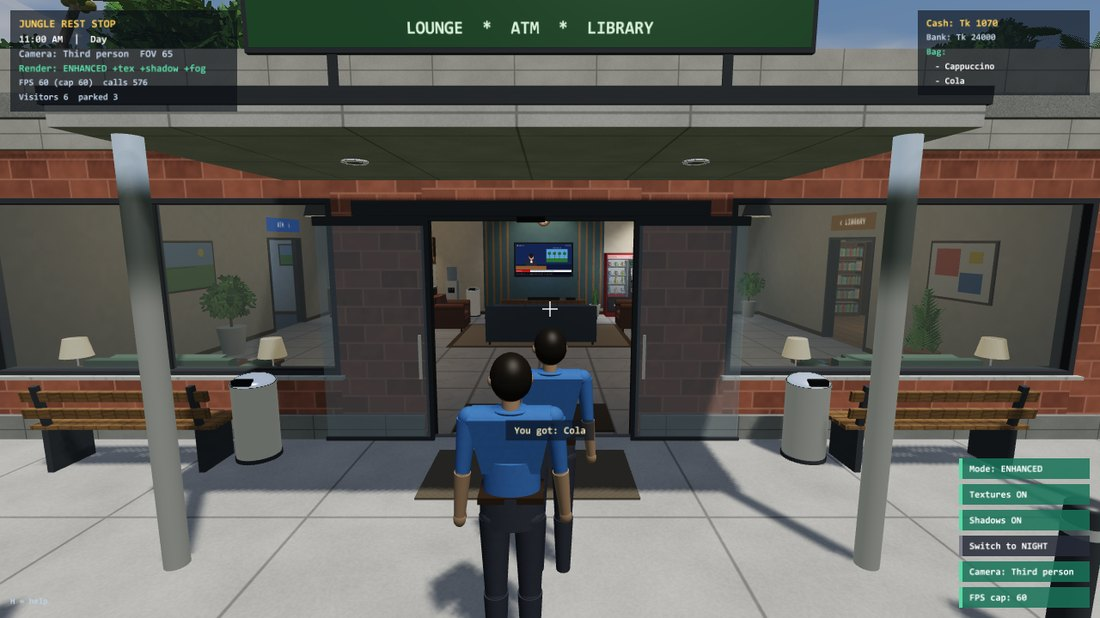
\includegraphics[width=\linewidth]{play_door}\caption{The sliding doors open in front of the player}\end{subfigure}
\begin{subfigure}{0.49\linewidth}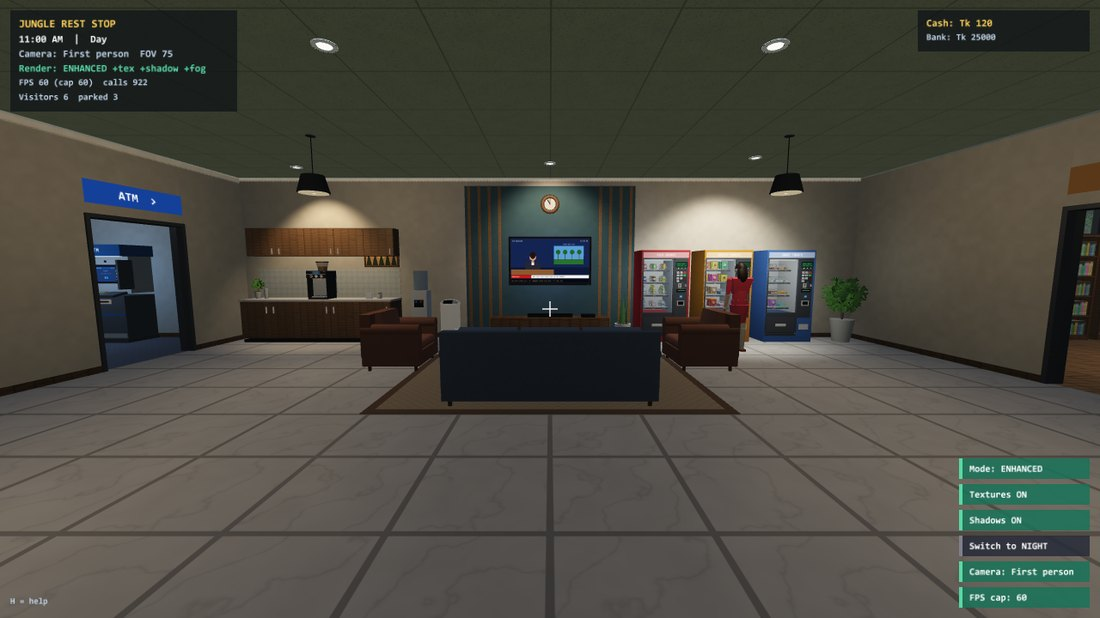
\includegraphics[width=\linewidth]{lounge_day}\caption{First person}\end{subfigure}
\begin{subfigure}{0.49\linewidth}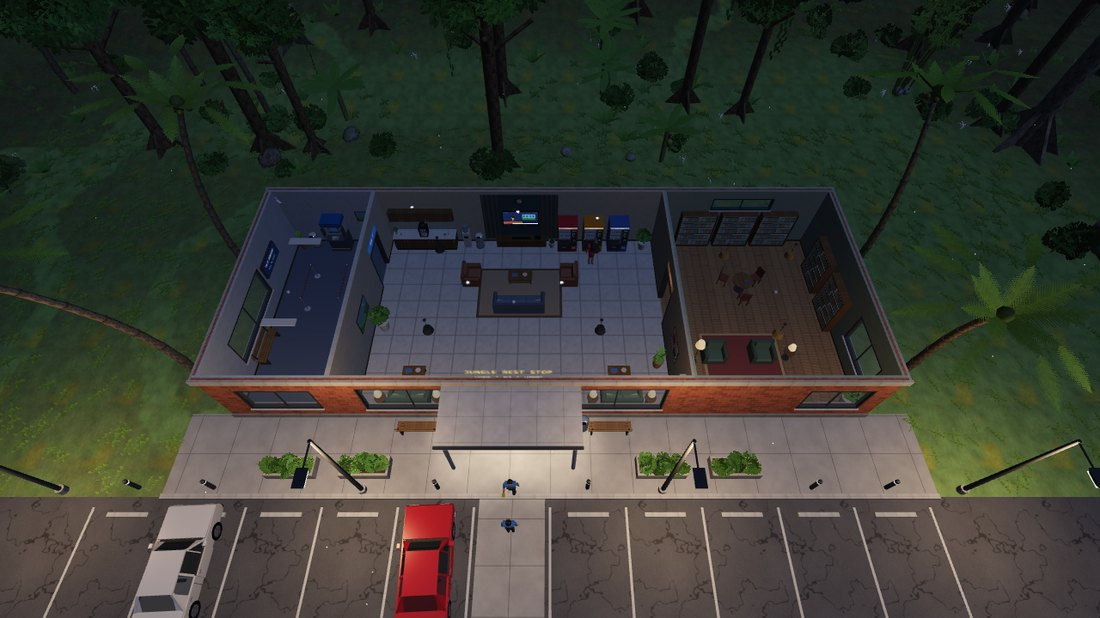
\includegraphics[width=\linewidth]{cutaway_night}\caption{Free camera, roof cut-away, night}\end{subfigure}
\begin{subfigure}{0.32\linewidth}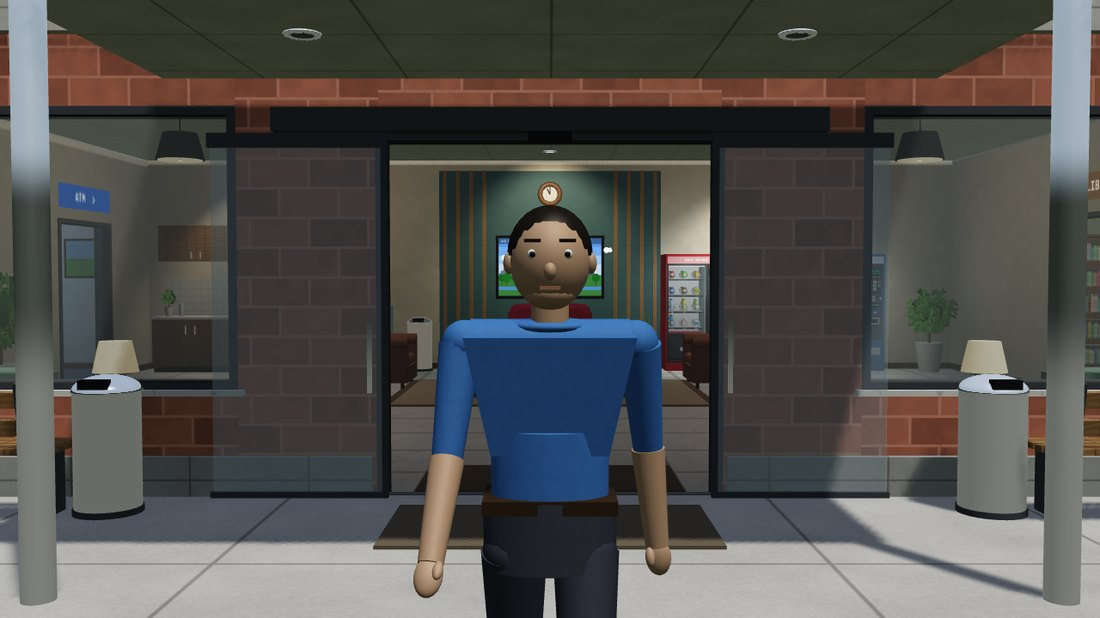
\includegraphics[width=\linewidth]{fov_35}\caption{FOV 35$^\circ$}\end{subfigure}
\begin{subfigure}{0.32\linewidth}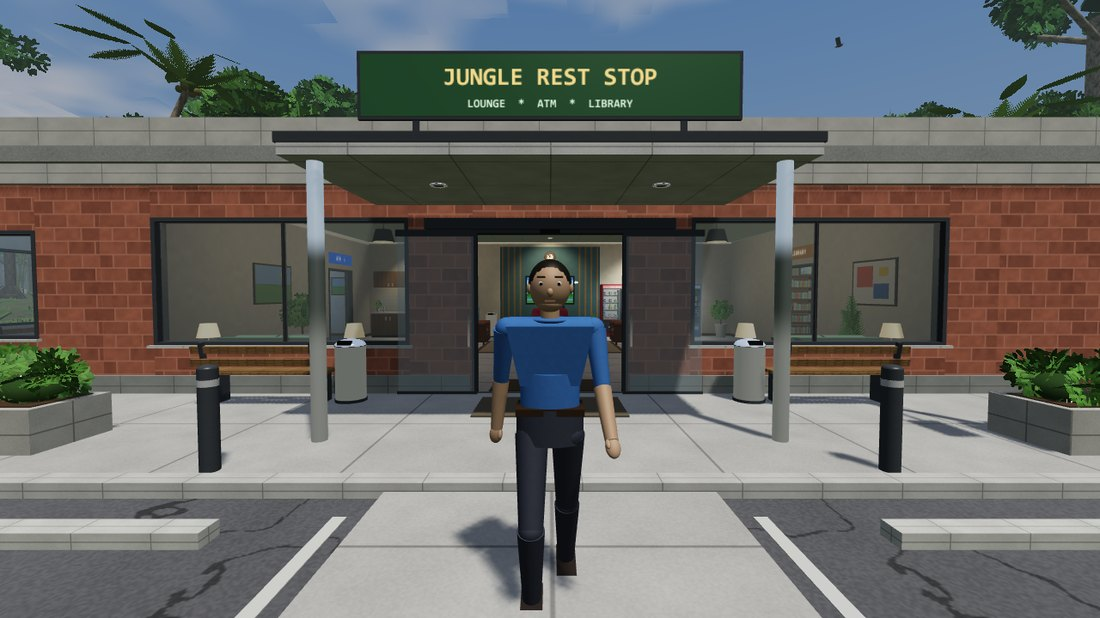
\includegraphics[width=\linewidth]{fov_70}\caption{FOV 70$^\circ$}\end{subfigure}
\begin{subfigure}{0.32\linewidth}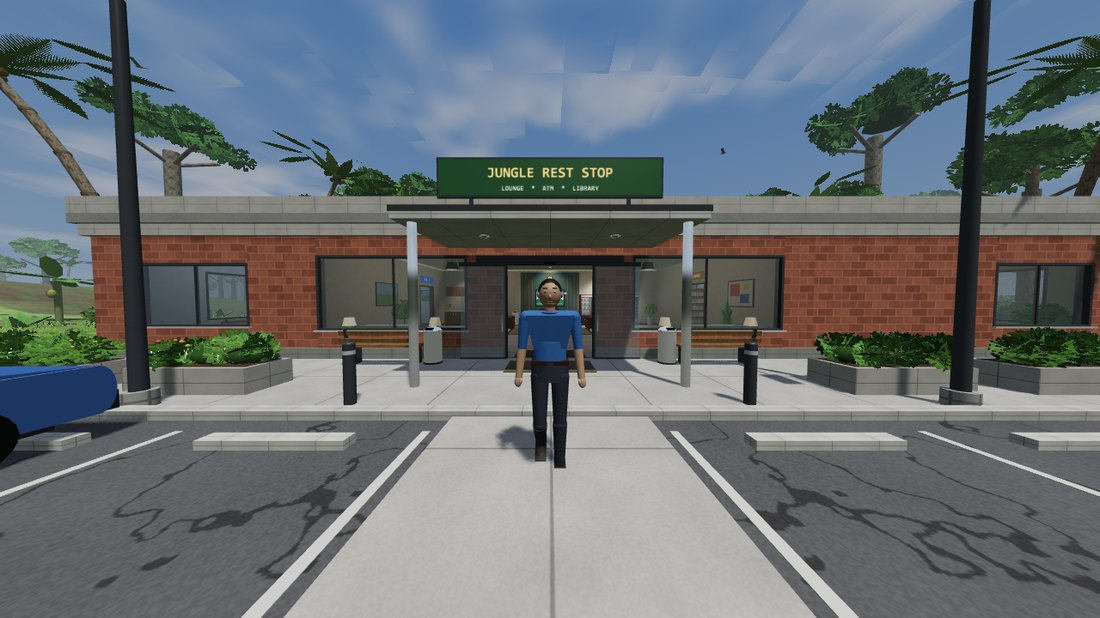
\includegraphics[width=\linewidth]{fov_100}\caption{FOV 100$^\circ$}\end{subfigure}
\caption{Camera modes and field of view.}\label{fig:cameras}
\end{figure}

\subsection{Object picking}
Every interactive part (buttons, slots, the flap, switches, the TV, the aquarium) registers an \emph{oriented box}
every frame: its matrix $M$ and its half size $\mathbf{h}$. A ray starts at the camera, $\mathbf{o}=\mathbf{e}$, and goes
through the centre of the screen in the view direction $\mathbf{d}$. For each box the ray is moved into the box's own
frame, $\mathbf{o}'=M^{-1}\mathbf{o}$, $\mathbf{d}'=M^{-1}\mathbf{d}$, and the \emph{slab test} is applied on each axis $a$:
\[
t_1=\frac{-h_a-o'_a}{d'_a},\quad t_2=\frac{h_a-o'_a}{d'_a},\qquad
t_{near}=\max_a\min(t_1,t_2),\quad t_{far}=\min_a\max(t_1,t_2).
\]
The ray hits the box if $t_{near}\le t_{far}$ and $0\le t_{near}\le 2.4$ m (the reach of an arm). The nearest hit wins: the
part is highlighted, its prompt is shown under the crosshair (for example ``Insert Tk 50 note''), and E runs its
action. The program checks this automatically by aiming the camera at fourteen parts and recording the prompt that
is found (\Cref{lst:probes}).
\lstinputlisting[language={},caption={Automatic picking test (part aimed at $\rightarrow$ prompt found)},label={lst:probes},basicstyle=\ttfamily\scriptsize]{generated/probes.txt}

\subsection{How the objects react}
\begin{table}[H]
\centering\small
\caption{Interactive parts and their reactions}\label{tab:reactions}
\begin{tabularx}{\linewidth}{@{}P{2.4cm}P{3.6cm}X P{2.0cm}@{}}
\toprule
Object & Part (prompt) & Reaction & Sound \\ \midrule
Vending machine & coin slot, note slot & credit +10 / +50 Tk, the cash in the wallet decreases & coin \\
 & keys A--D, 1--3, CLR, OK & the key moves in by 7 mm; the LCD shows the code, the price and the credit & click \\
 & collection flap & swings in by $R_x(50^\circ)$; the item goes into the bag & click \\
 & coin cup, return lever & the change is collected; the credit is returned & coin \\
ATM & card slot & the card slides in or out & click \\
 & keypad, side keys & PIN stars, menu choice, amount (\Cref{fig:atmsm}) & beep \\
 & cash dispenser, receipt & notes slide out, cash goes to the wallet; the receipt curls out & cash \\
Coffee machine & three buttons, cup & cup drops, grinding, pouring, steam; the drink goes into the bag & grinder, pour, beep \\
Television & screen & next channel with a short static noise & click \\
Aquarium & glass & food crumbs sink and the fish swim up & click \\
Light switch & switch & the rocker flips; the lamps of the group and their lights switch & click \\
Entrance & (no key) & the doors slide open when a person is near & whoosh \\
\bottomrule
\end{tabularx}
\end{table}

\subsubsection{Buying from a vending machine}
\Cref{fig:playvend} follows one purchase from the player's eyes. The HUD shows the prompt of the part under the
crosshair, the cash in the wallet and the items in the bag (top right).
\begin{figure}[H]
\centering
\begin{subfigure}{0.49\linewidth}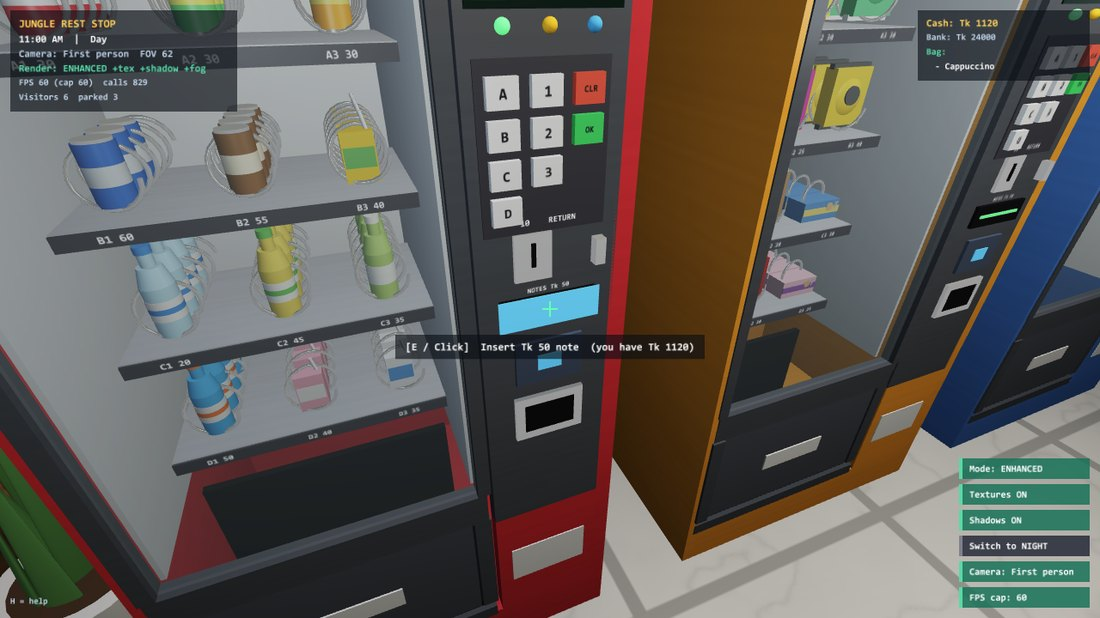
\includegraphics[width=\linewidth]{play_1_look}\caption{Looking at the note slot: ``Insert Tk 50 note''}\end{subfigure}
\begin{subfigure}{0.49\linewidth}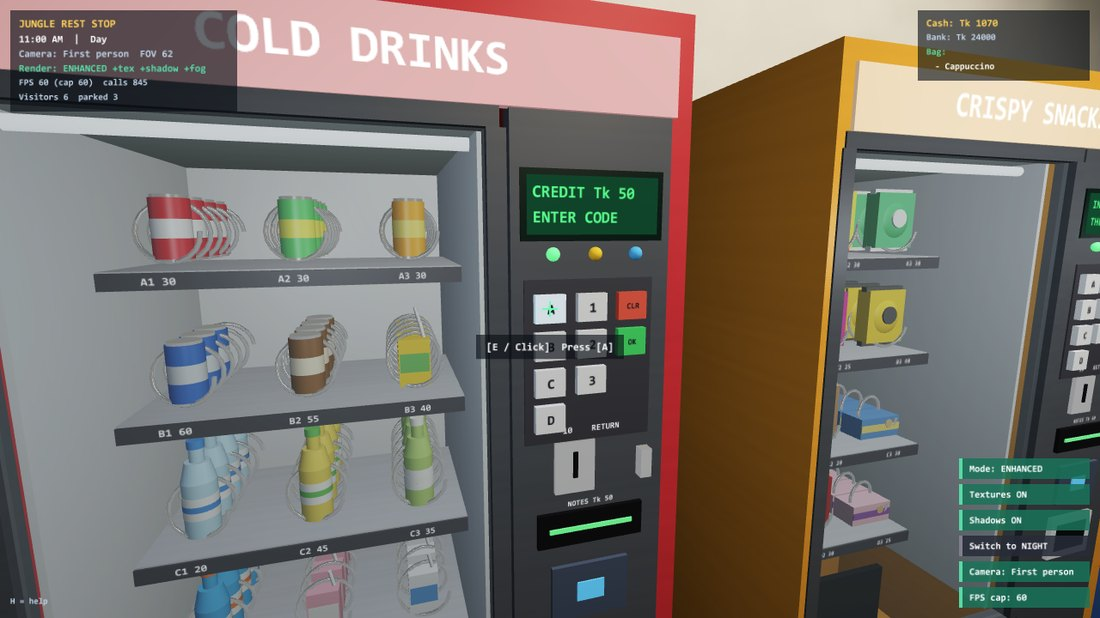
\includegraphics[width=\linewidth]{play_2_coin}\caption{Credit Tk 50 on the LCD; aiming at key A}\end{subfigure}
\begin{subfigure}{0.49\linewidth}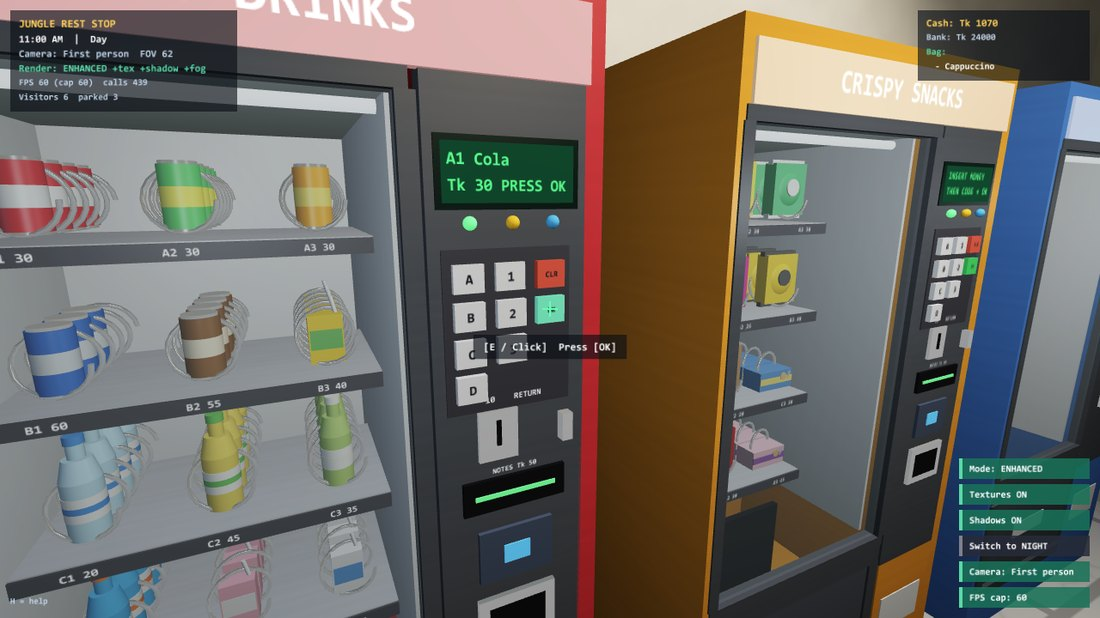
\includegraphics[width=\linewidth]{play_3_code}\caption{Code A1 (Cola, Tk 30) typed; aiming at OK}\end{subfigure}
\begin{subfigure}{0.49\linewidth}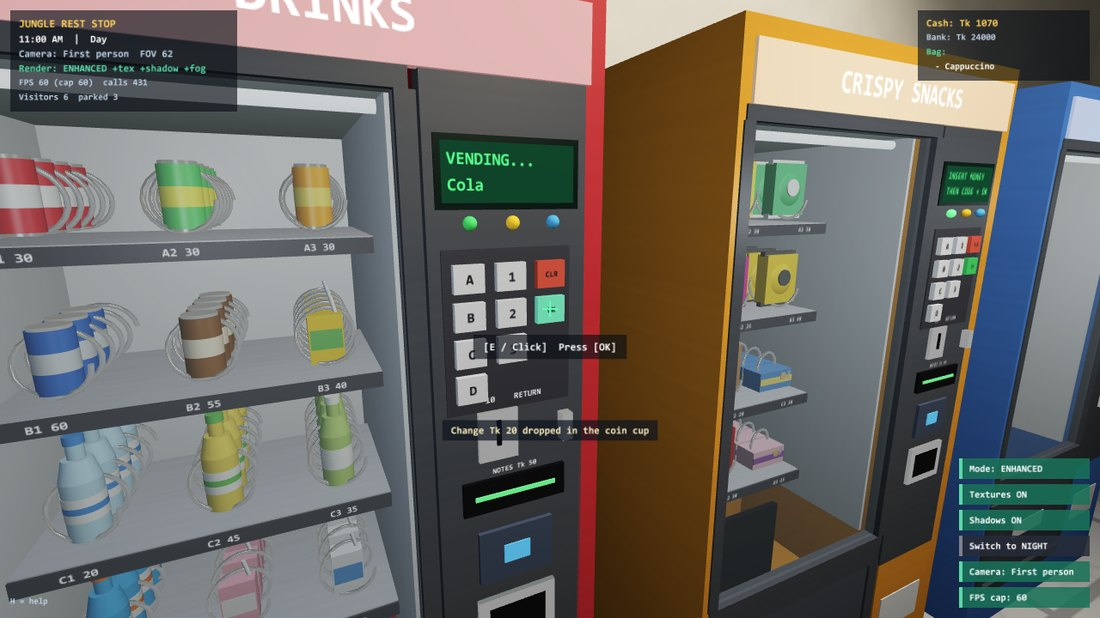
\includegraphics[width=\linewidth]{play_4_spiral}\caption{The spiral turns and pushes the can forward}\end{subfigure}
\begin{subfigure}{0.49\linewidth}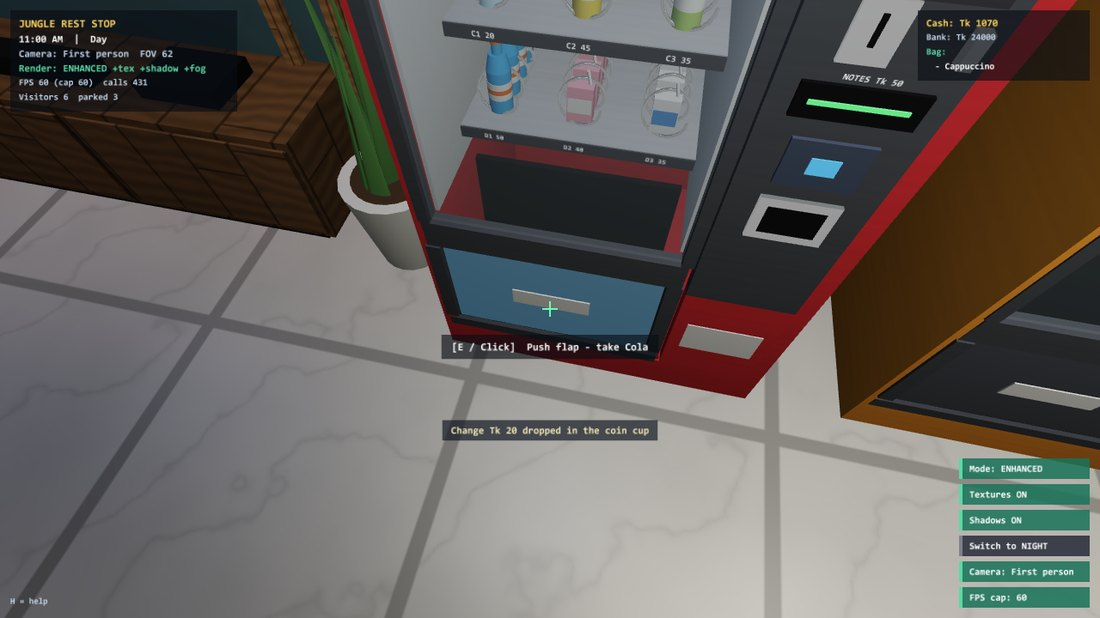
\includegraphics[width=\linewidth]{play_5_drop}\caption{The can lies in the tray: ``Push flap''}\end{subfigure}
\begin{subfigure}{0.49\linewidth}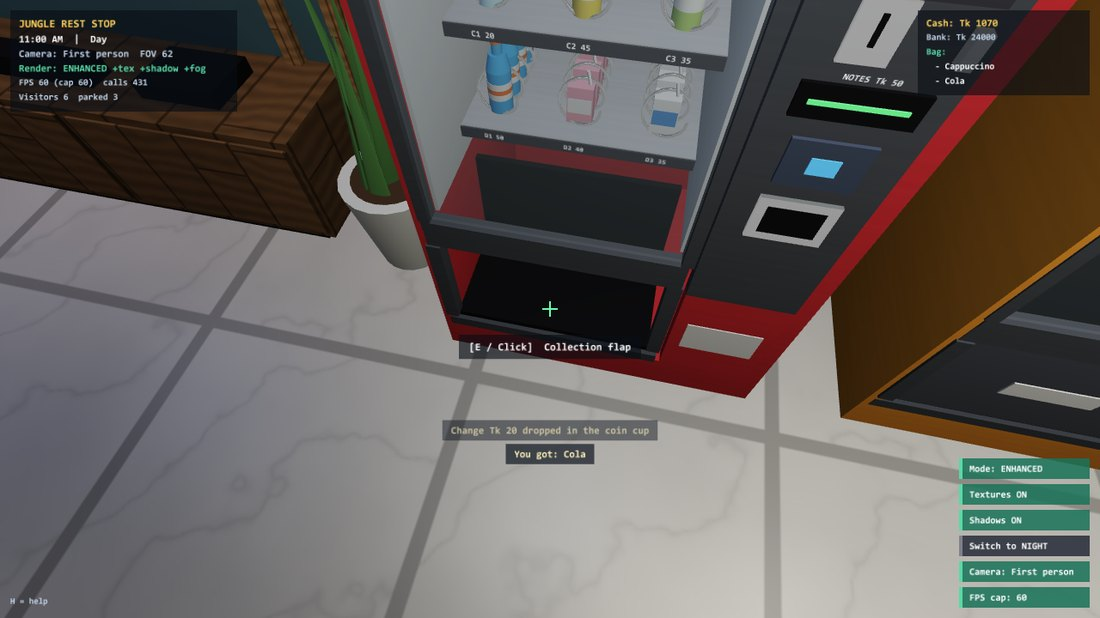
\includegraphics[width=\linewidth]{play_6_flap}\caption{The flap swings in; the can is in the bag, Tk 20 change in the cup}\end{subfigure}
\caption{The player buys a can of Cola.}\label{fig:playvend}
\end{figure}
\begin{figure}[H]
\centering
\begin{subfigure}{0.32\linewidth}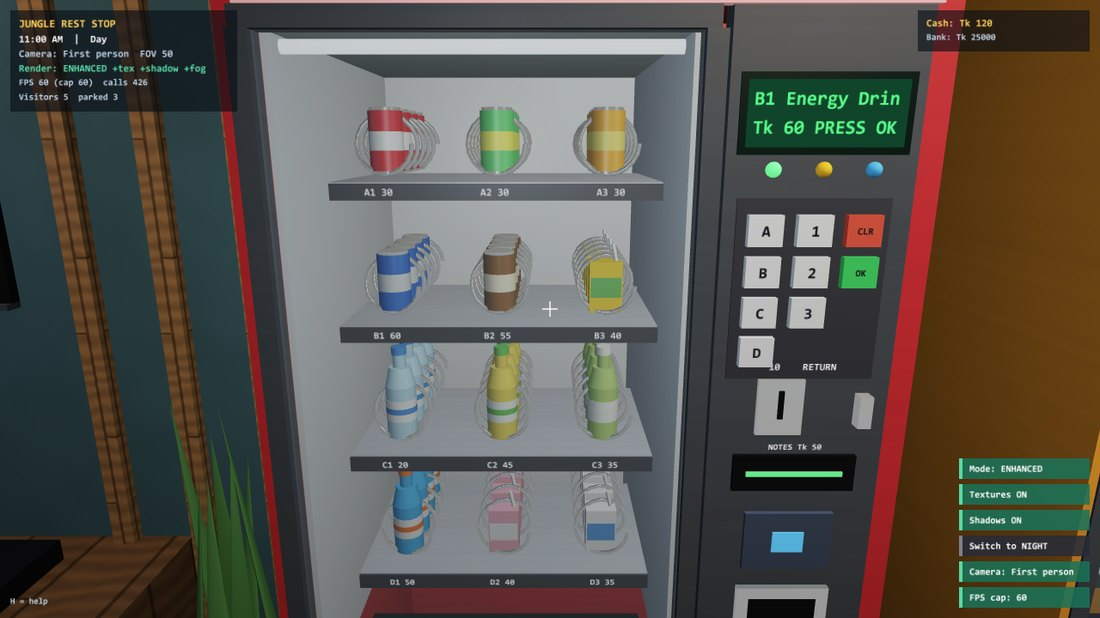
\includegraphics[width=\linewidth]{vending_code}\caption{Code typed, credit enough}\end{subfigure}
\begin{subfigure}{0.32\linewidth}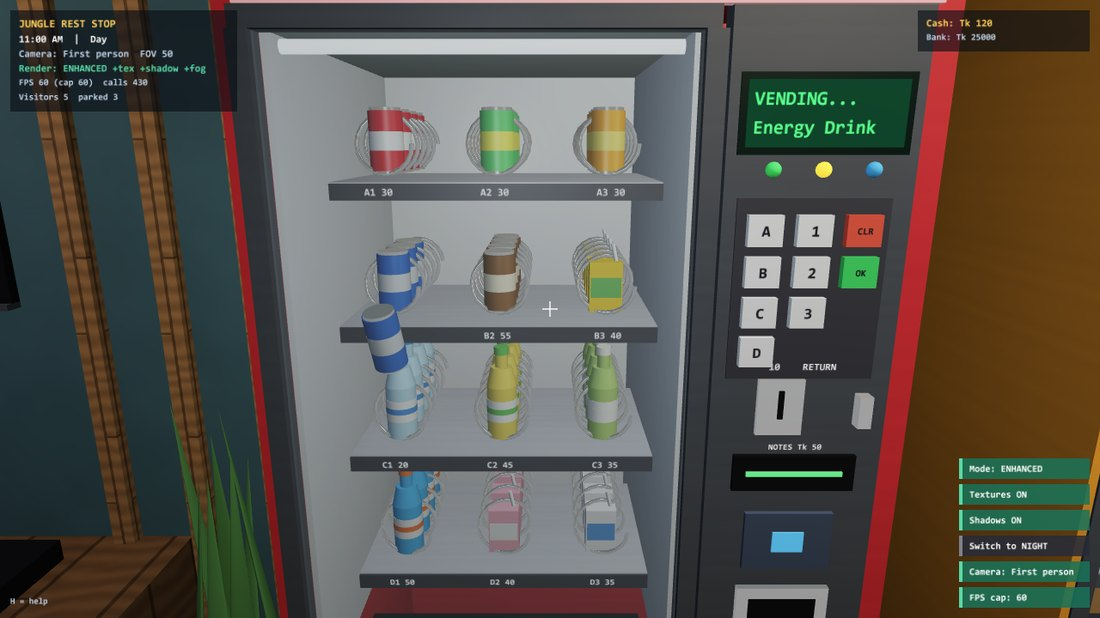
\includegraphics[width=\linewidth]{vending_dispense}\caption{The product falls}\end{subfigure}
\begin{subfigure}{0.32\linewidth}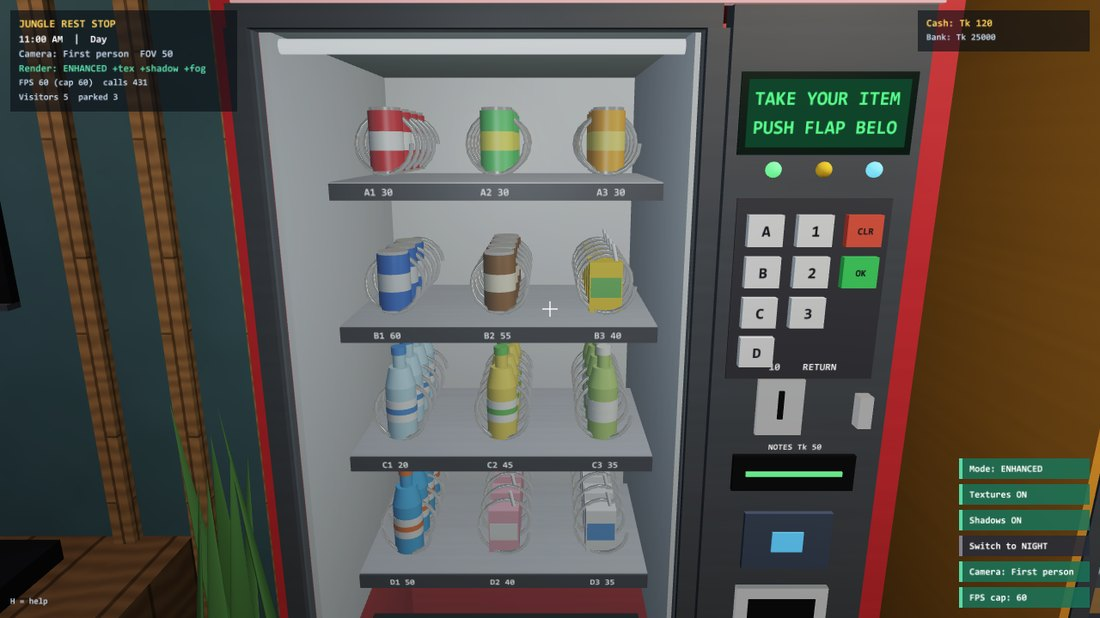
\includegraphics[width=\linewidth]{vending_ready}\caption{``Take your item''}\end{subfigure}
\caption{The same steps seen closer, with the downlight (spot light) above the machine.}\label{fig:vendbuy}
\end{figure}

\subsubsection{Using the ATM}
\begin{figure}[H]
\centering
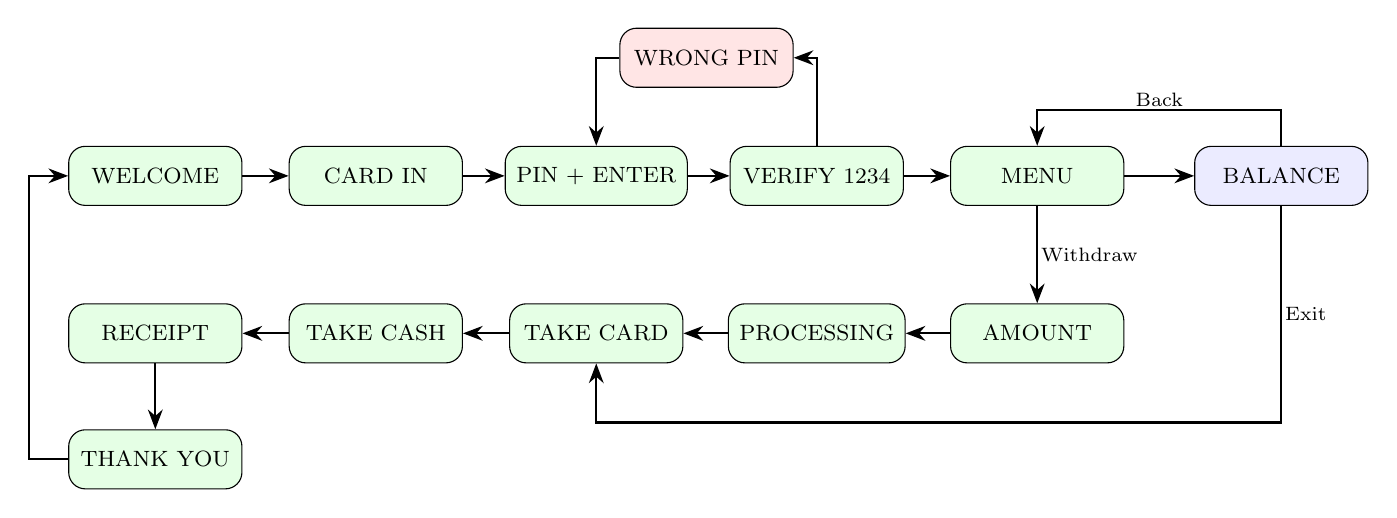
\begin{tikzpicture}[state/.append style={minimum width=2.2cm,minimum height=0.75cm,font=\footnotesize},lb/.style={font=\scriptsize,fill=white,inner sep=1pt}]
\node[state] (w) at (0,0) {WELCOME};
\node[state] (c) at (2.8,0) {CARD IN};
\node[state] (p) at (5.6,0) {PIN + ENTER};
\node[state] (v) at (8.4,0) {VERIFY 1234};
\node[state] (m) at (11.2,0) {MENU};
\node[state=blue!8] (b) at (14.3,0) {BALANCE};
\node[state=red!10] (wr) at (7.0,1.5) {WRONG PIN};
\node[state] (a) at (11.2,-2.0) {AMOUNT};
\node[state] (pr) at (8.4,-2.0) {PROCESSING};
\node[state] (tc) at (5.6,-2.0) {TAKE CARD};
\node[state] (tm) at (2.8,-2.0) {TAKE CASH};
\node[state] (r) at (0,-2.0) {RECEIPT};
\node[state] (t) at (0,-3.6) {THANK YOU};
\draw[arr] (w)--(c); \draw[arr] (c)--(p); \draw[arr] (p)--(v); \draw[arr] (v)--(m);
\draw[arr] (v.north) |- (wr.east);
\draw[arr] (wr.west) -| (p.north);
\draw[arr] (m)--node[lb,right]{Withdraw}(a);
\draw[arr] (m)--(b);
\draw[arr] (b.north) -- ++(0,0.45) -| node[lb,above,pos=0.25]{Back} (m.north);
\draw[arr] (b.south) |- node[lb,pos=0.25,right]{Exit} ([yshift=-0.75cm]tc.south) -- (tc.south);
\draw[arr] (a)--(pr); \draw[arr] (pr)--(tc); \draw[arr] (tc)--(tm); \draw[arr] (tm)--(r); \draw[arr] (r)--(t);
\draw[arr] (t.west) -- ++(-0.5,0) |- (w.west);
\end{tikzpicture}
\caption{ATM state machine. CANCEL at any step leads to TAKE CARD; the card is always returned before the cash.}\label{fig:atmsm}
\end{figure}
The eight steps are listed in a HUD panel and the current step is highlighted. Inside the machine the card slides in
and out, the PIN appears as stars, the notes slide out of the dispenser and the receipt curls out of the printer.
\begin{figure}[H]
\centering
\begin{subfigure}{0.32\linewidth}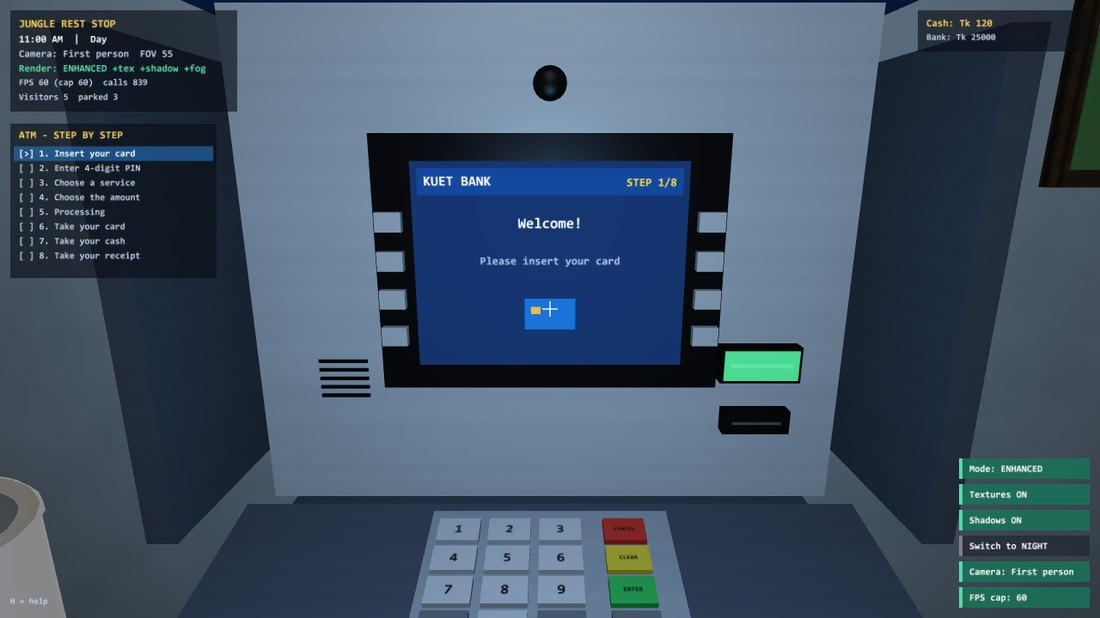
\includegraphics[width=\linewidth]{atm_1_welcome}\caption{1. Insert card}\end{subfigure}
\begin{subfigure}{0.32\linewidth}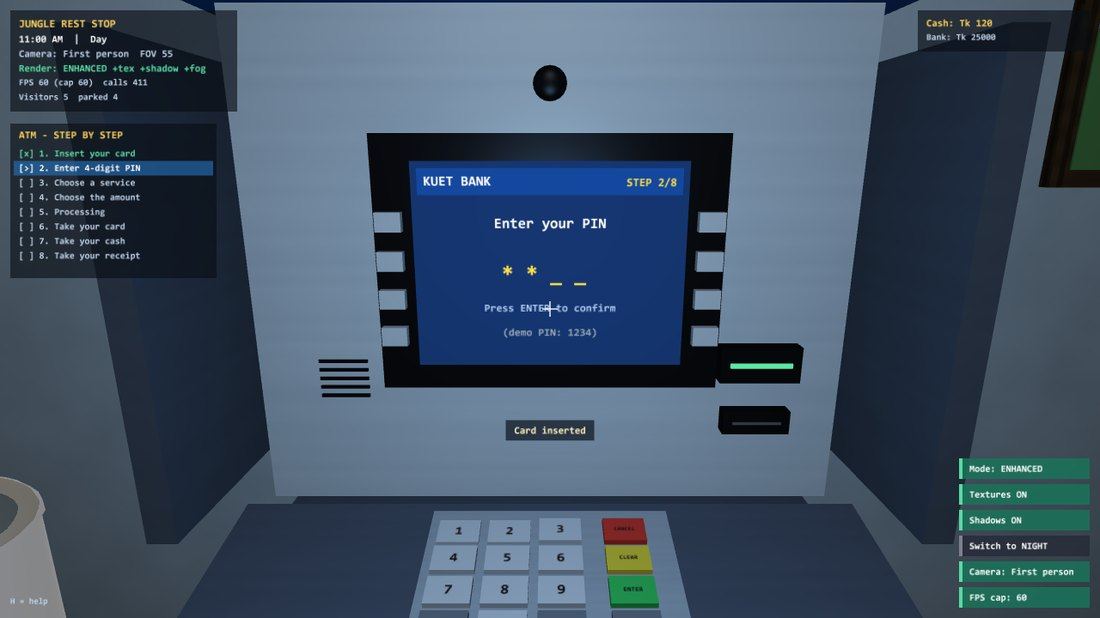
\includegraphics[width=\linewidth]{atm_2_pin}\caption{2. Enter PIN}\end{subfigure}
\begin{subfigure}{0.32\linewidth}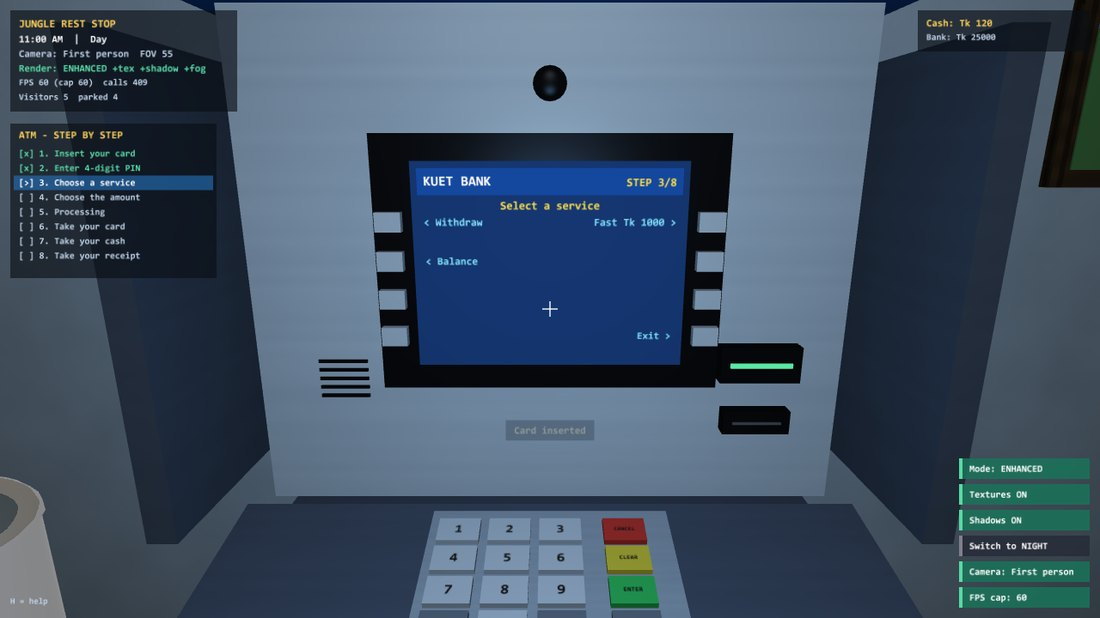
\includegraphics[width=\linewidth]{atm_3_menu}\caption{3. Choose a service}\end{subfigure}
\begin{subfigure}{0.32\linewidth}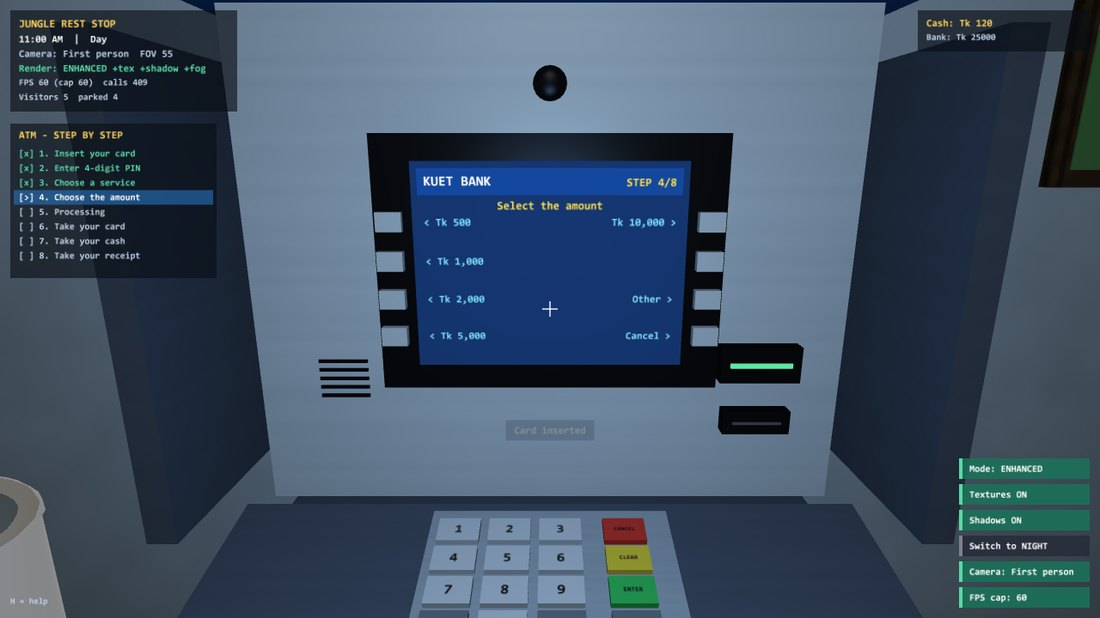
\includegraphics[width=\linewidth]{atm_4_amount}\caption{4. Choose amount}\end{subfigure}
\begin{subfigure}{0.32\linewidth}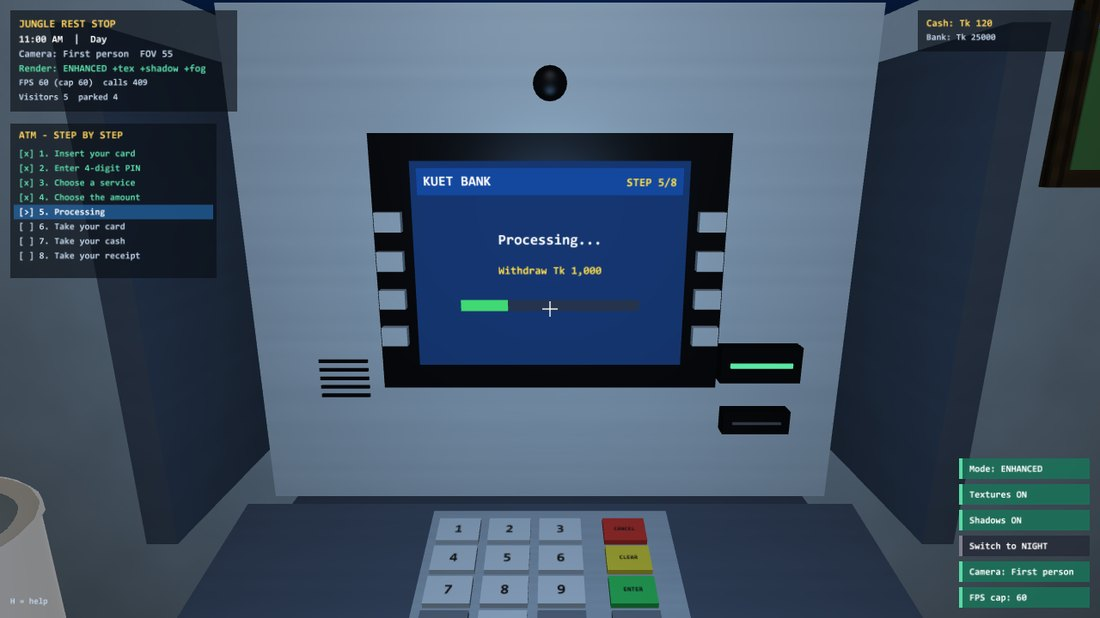
\includegraphics[width=\linewidth]{atm_5_processing}\caption{5. Processing}\end{subfigure}
\begin{subfigure}{0.32\linewidth}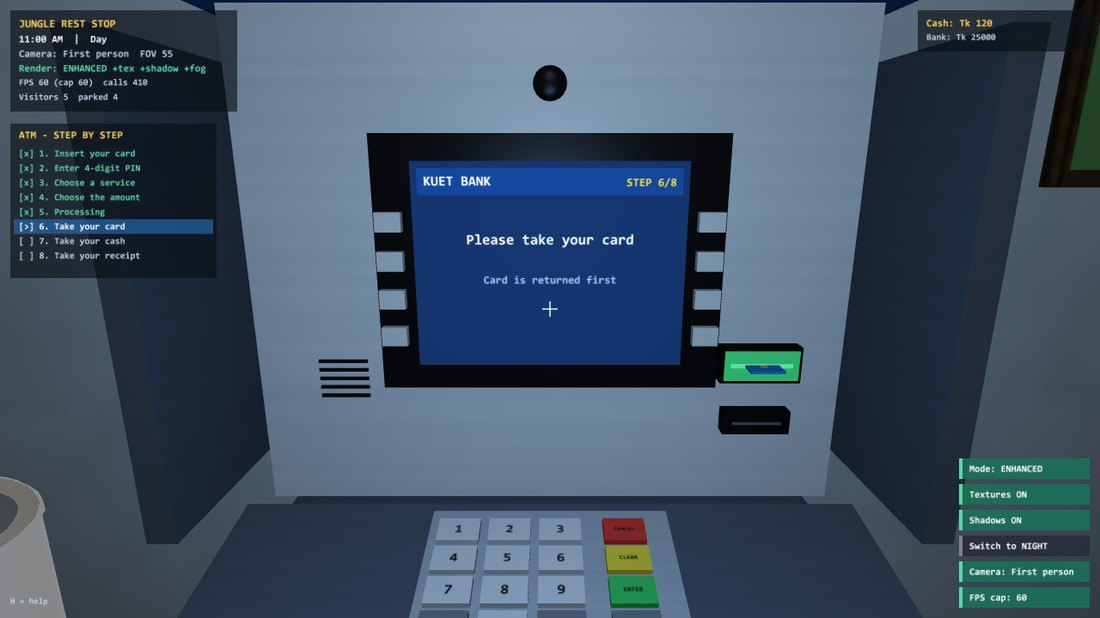
\includegraphics[width=\linewidth]{atm_6_takecard}\caption{6. Take card}\end{subfigure}
\begin{subfigure}{0.32\linewidth}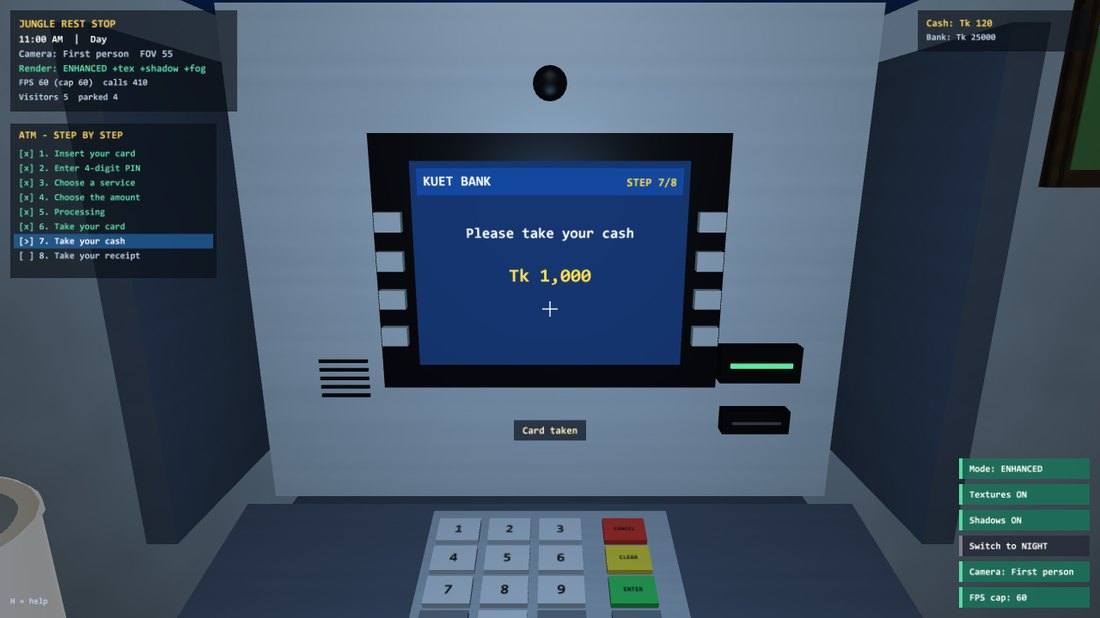
\includegraphics[width=\linewidth]{atm_7_takecash}\caption{7. Take cash}\end{subfigure}
\begin{subfigure}{0.32\linewidth}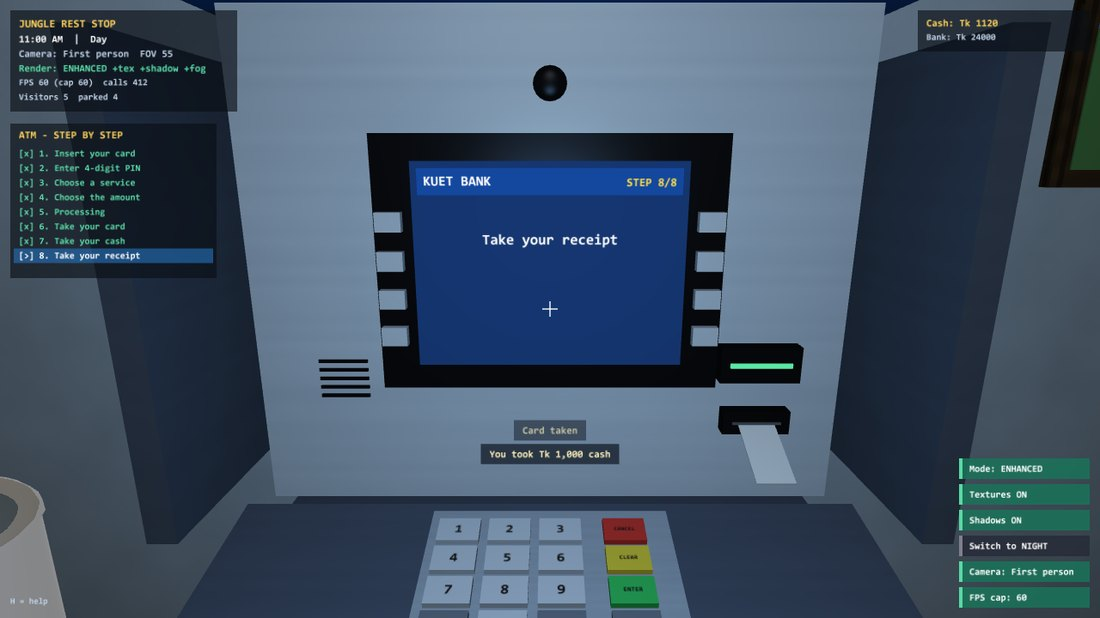
\includegraphics[width=\linewidth]{atm_8_receipt}\caption{8. Take receipt}\end{subfigure}
\begin{subfigure}{0.32\linewidth}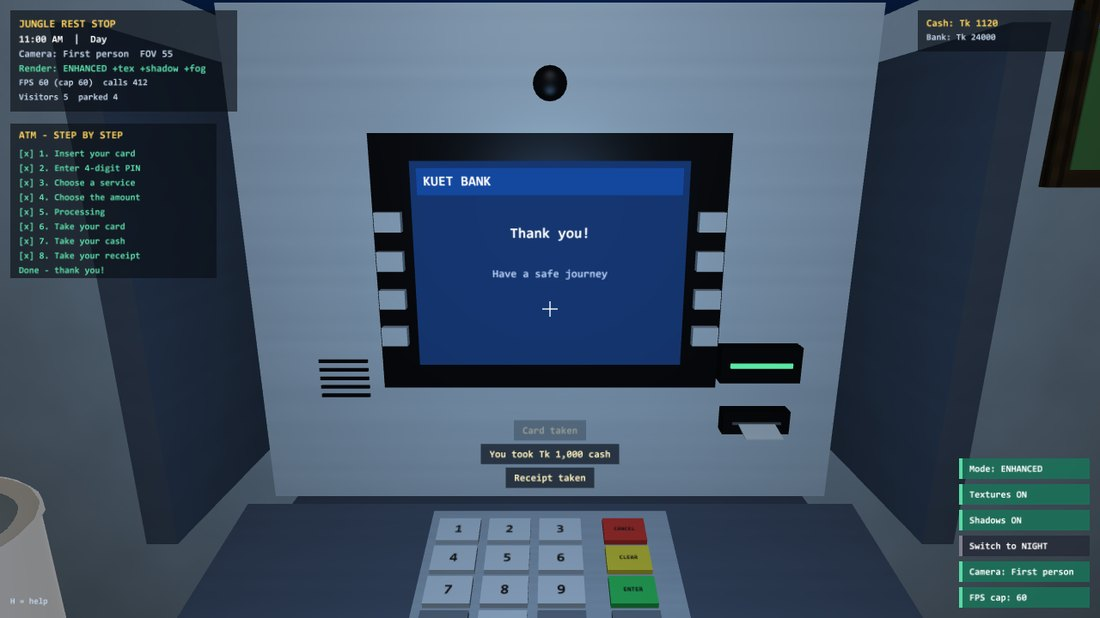
\includegraphics[width=\linewidth]{atm_9_thanks}\caption{Done}\end{subfigure}
\caption{A withdrawal of Tk 1,000 with the step list on the left.}
\end{figure}

\subsubsection{Coffee machine, television, light switch and aquarium}
\begin{figure}[H]
\centering
\begin{subfigure}{0.49\linewidth}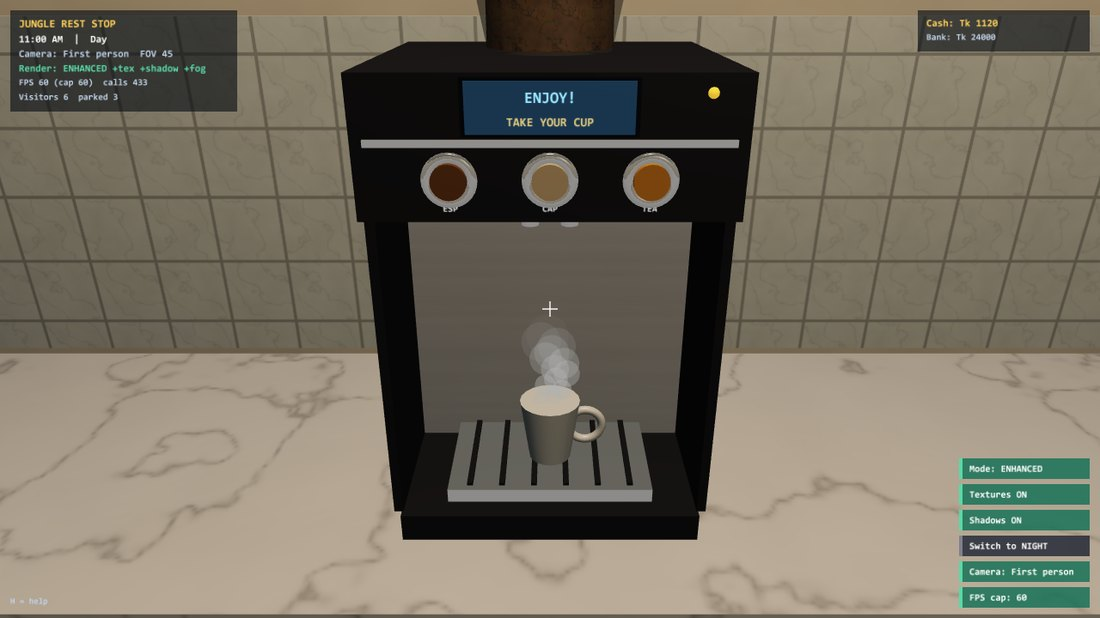
\includegraphics[width=\linewidth]{coffee_brewing}\caption{Brewing a cappuccino (stream, rising coffee, steam)}\end{subfigure}
\begin{subfigure}{0.49\linewidth}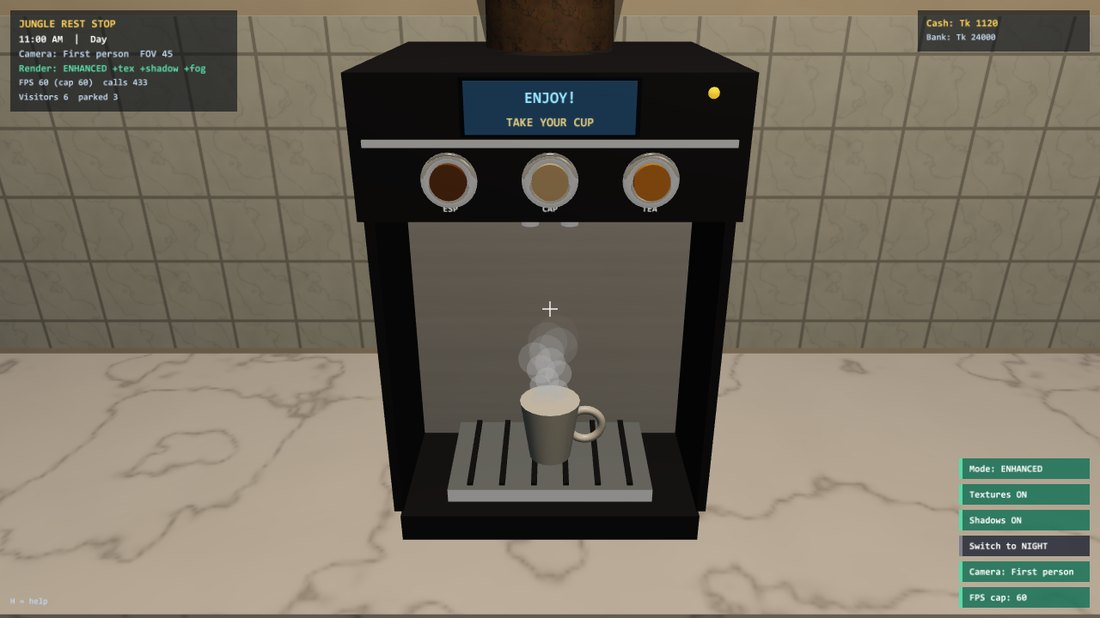
\includegraphics[width=\linewidth]{coffee_ready}\caption{Ready: take the cup}\end{subfigure}
\begin{subfigure}{0.49\linewidth}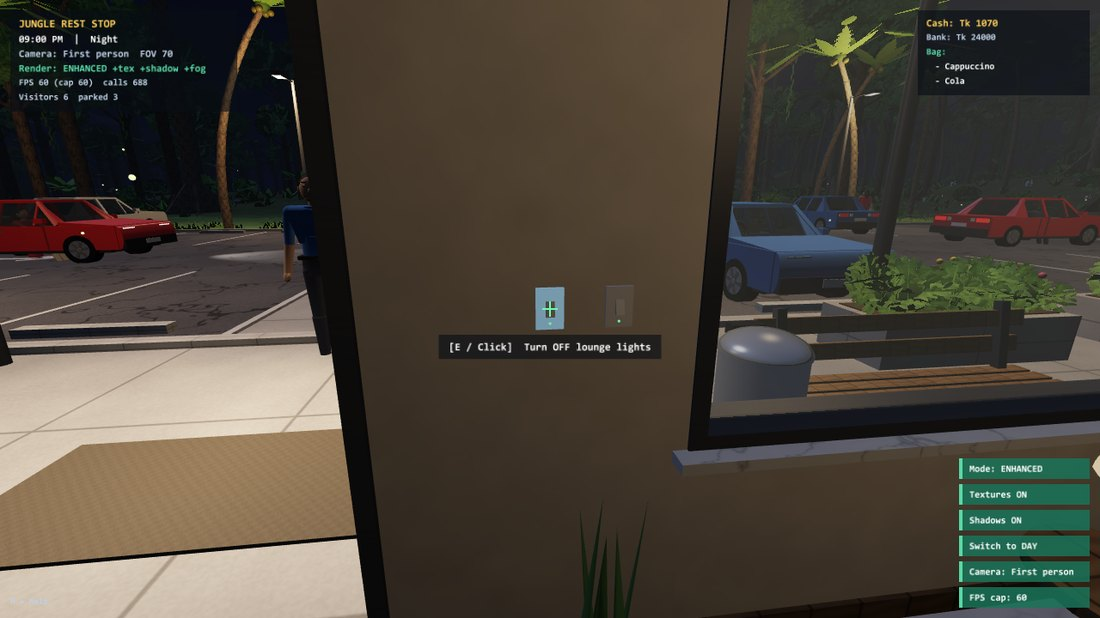
\includegraphics[width=\linewidth]{play_switch_on}\caption{Night: looking at the lounge light switch}\end{subfigure}
\begin{subfigure}{0.49\linewidth}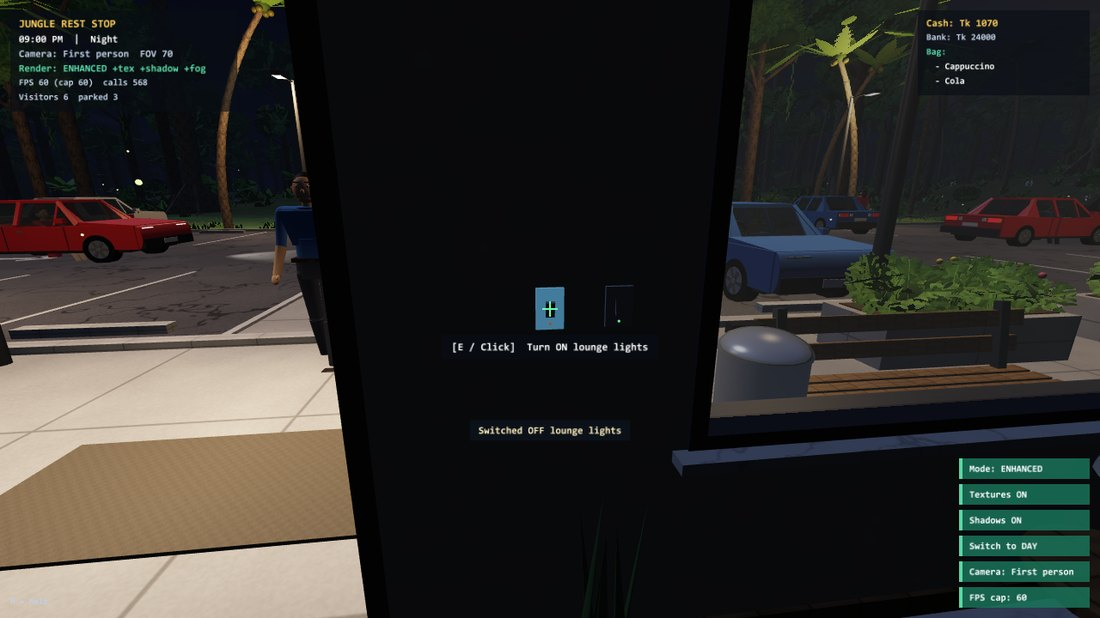
\includegraphics[width=\linewidth]{play_switch_off}\caption{After pressing E: the lounge lights are off}\end{subfigure}
\begin{subfigure}{0.49\linewidth}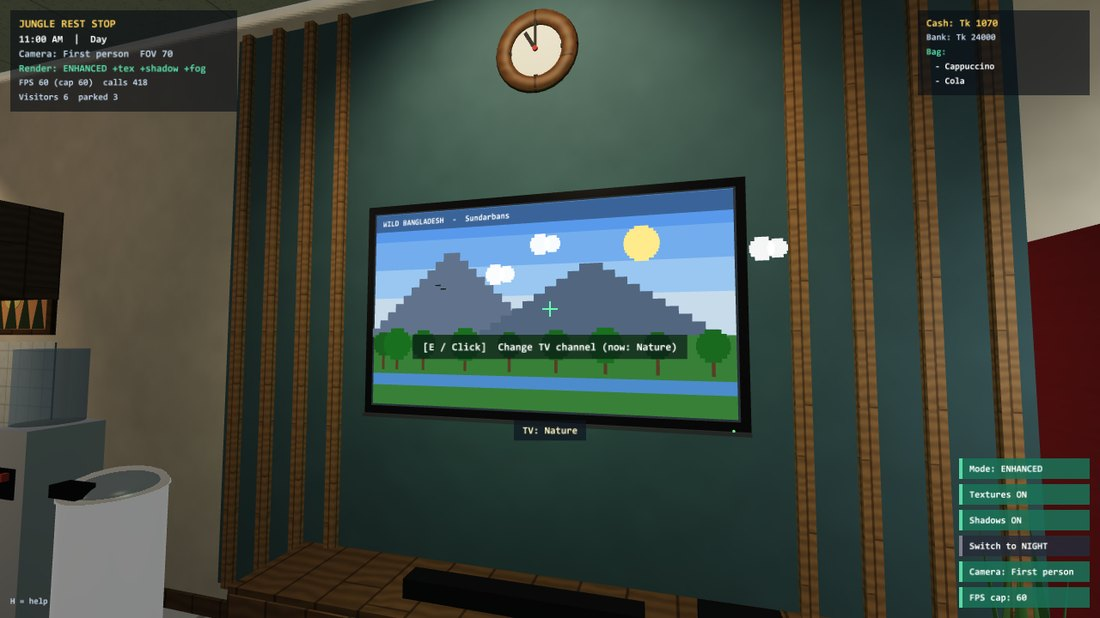
\includegraphics[width=\linewidth]{play_tv}\caption{Changing the TV channel}\end{subfigure}
\begin{subfigure}{0.49\linewidth}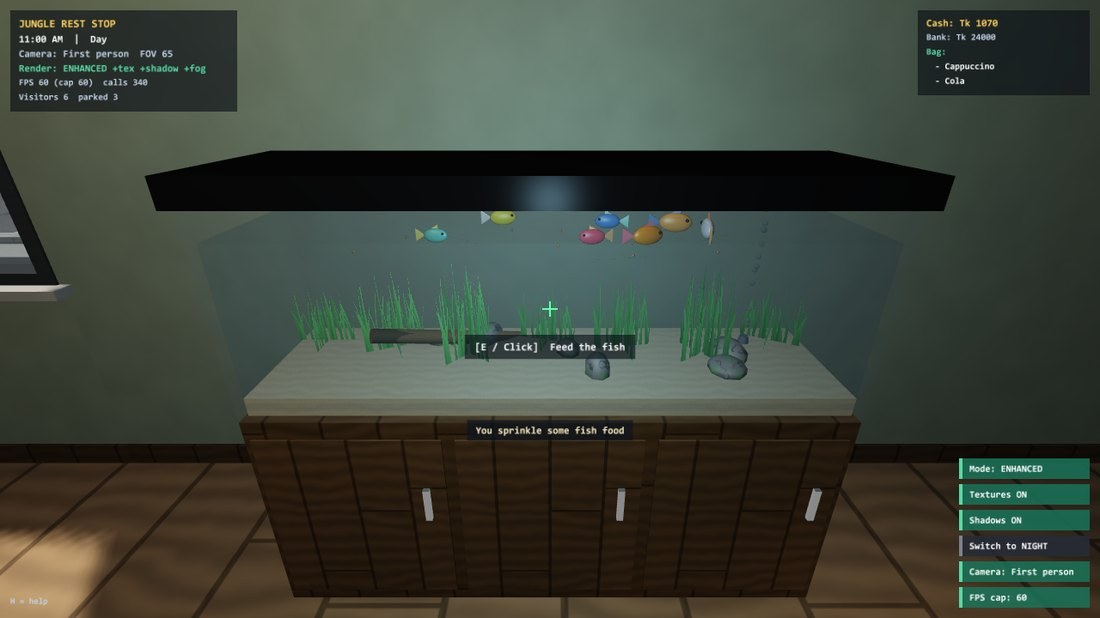
\includegraphics[width=\linewidth]{play_fish}\caption{Feeding the fish: they swim up to the food}\end{subfigure}
\caption{Reactions of the coffee machine, the light switch, the TV and the aquarium.}
\end{figure}
\begin{figure}[H]
\centering
\begin{subfigure}{0.24\linewidth}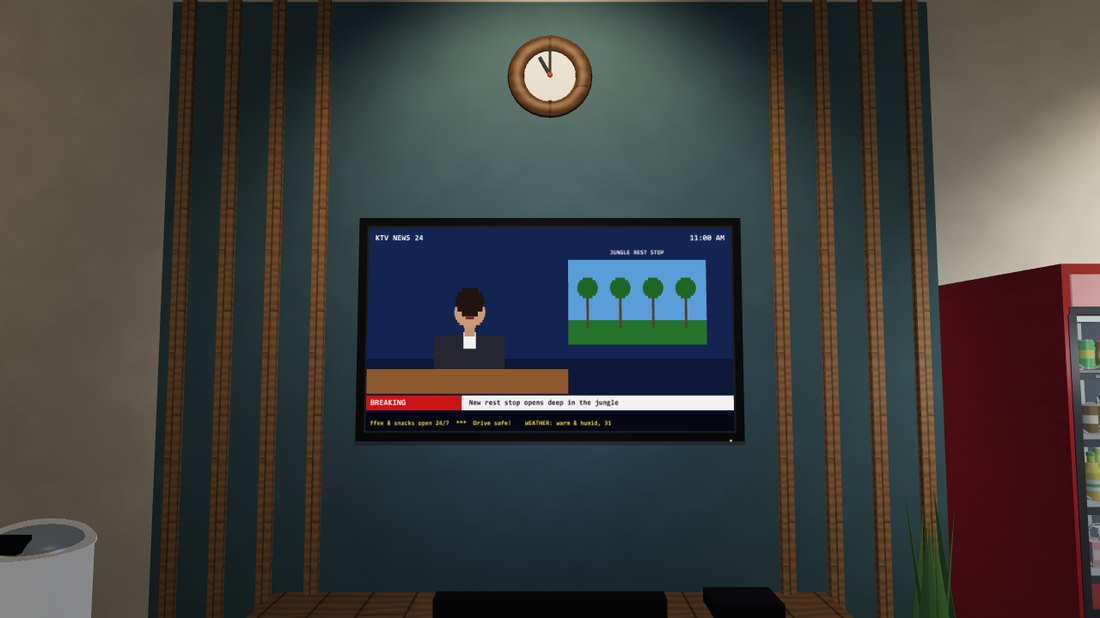
\includegraphics[width=\linewidth]{tv_ch1}\caption{News + ticker}\end{subfigure}
\begin{subfigure}{0.24\linewidth}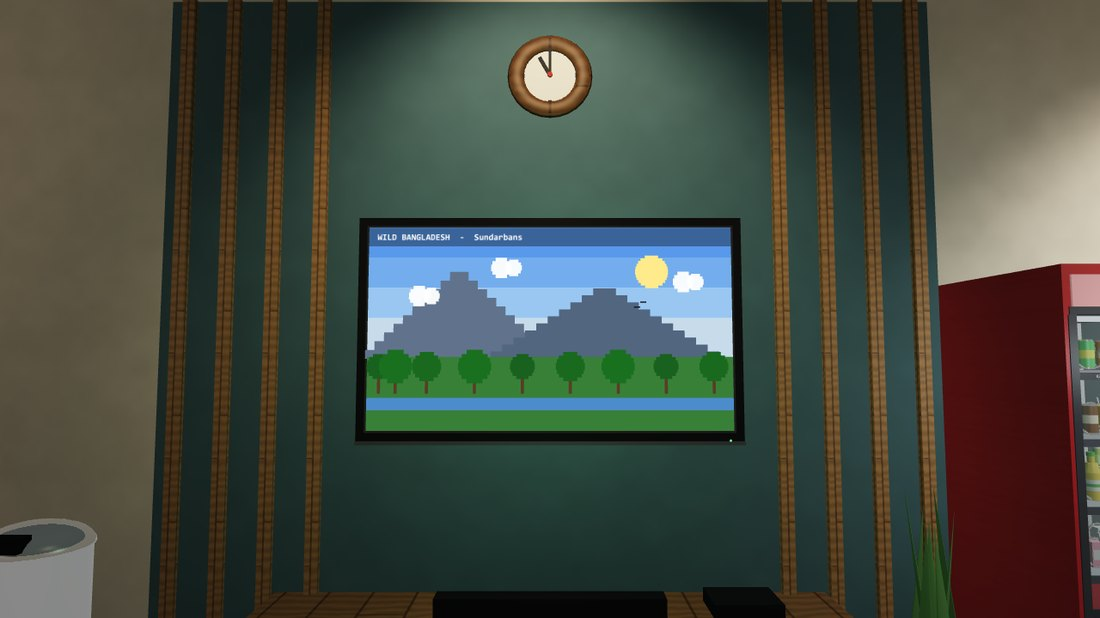
\includegraphics[width=\linewidth]{tv_ch2}\caption{Nature}\end{subfigure}
\begin{subfigure}{0.24\linewidth}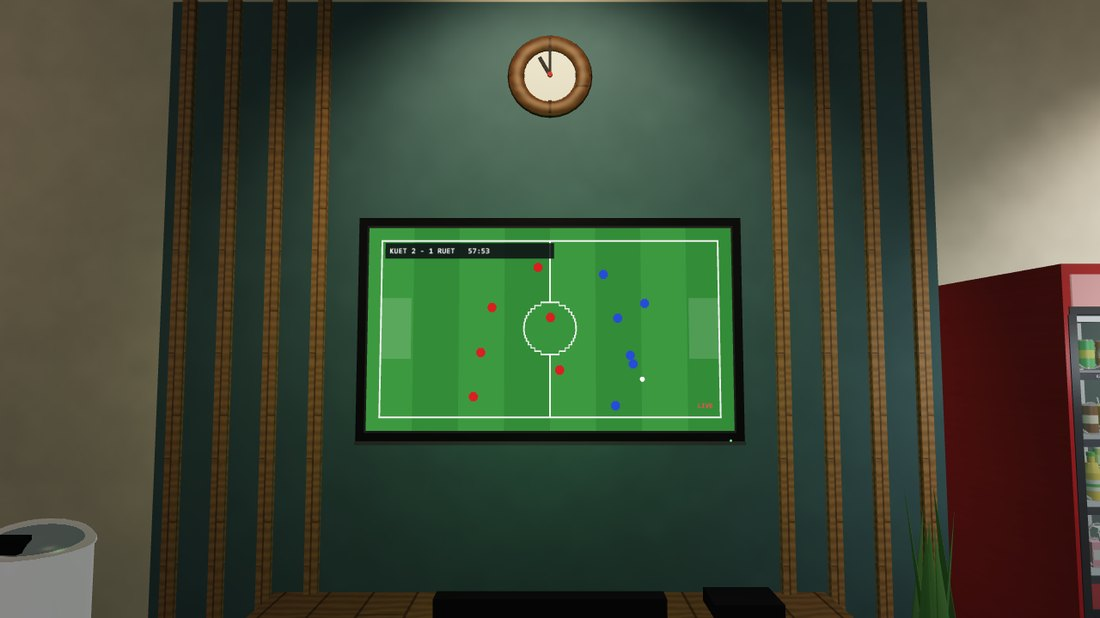
\includegraphics[width=\linewidth]{tv_ch3}\caption{Live football}\end{subfigure}
\begin{subfigure}{0.24\linewidth}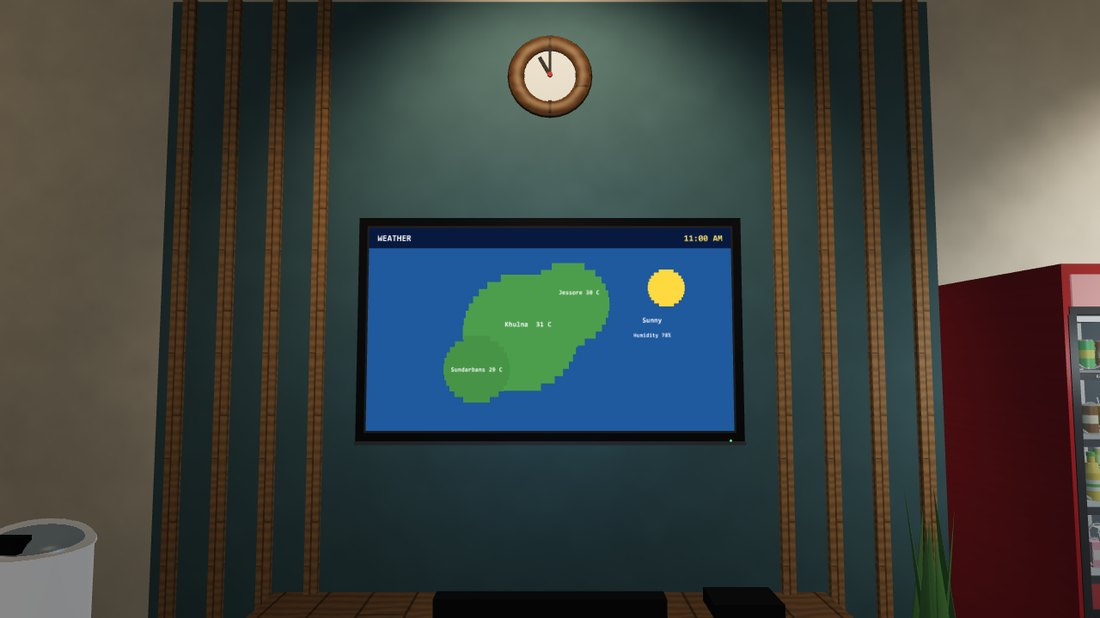
\includegraphics[width=\linewidth]{tv_ch4}\caption{Weather (game time)}\end{subfigure}
\caption{The four animated TV channels.}
\end{figure}

% =============================================================================
\section{NPC Visitors}\label{sec:npc}
\subsection{Visitor life cycle}
Visitors appear only inside a car at the far end of the road. A new car comes every 8--18 s when a parking spot is
free and the road entrance is clear; at most six visitors are active at once. Every visitor is a state machine
(\Cref{fig:visitorsm}).
\begin{figure}[H]
\centering
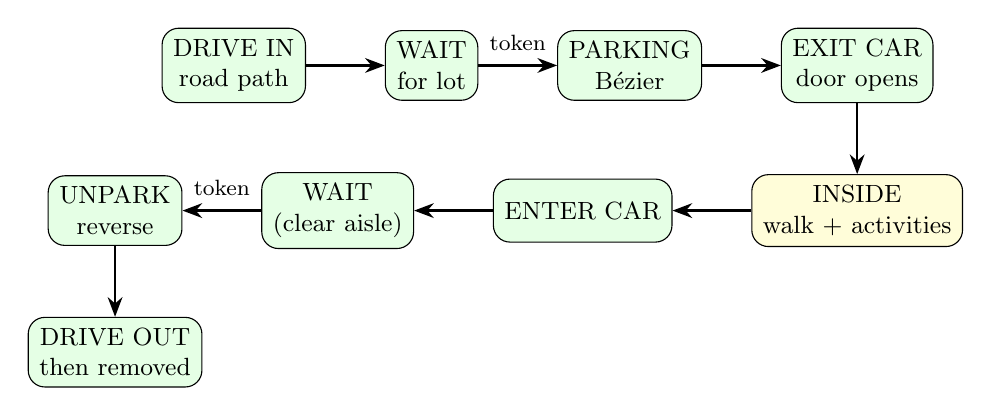
\begin{tikzpicture}[node distance=0.9cm and 1.0cm]
\node[state] (a) {DRIVE IN\\road path};
\node[state,right=of a] (b) {WAIT\\for lot};
\node[state,right=of b] (c) {PARKING\\B\'ezier};
\node[state,right=of c] (d) {EXIT CAR\\door opens};
\node[state=yellow!15,below=0.9cm of d] (e) {INSIDE\\walk + activities};
\node[state,left=of e] (f) {ENTER CAR};
\node[state,left=of f] (g) {WAIT\\(clear aisle)};
\node[state,left=of g] (h) {UNPARK\\reverse};
\node[state,below=0.9cm of h] (i) {DRIVE OUT\\then removed};
\draw[arr] (a)--(b); \draw[arr] (b)--node[lbl,above=4pt]{token}(c); \draw[arr] (c)--(d); \draw[arr] (d)--(e);
\draw[arr] (e)--(f); \draw[arr] (f)--(g); \draw[arr] (g)--node[lbl,above=4pt]{token}(h); \draw[arr] (h)--(i);
\end{tikzpicture}
\caption{Visitor state machine.}\label{fig:visitorsm}
\end{figure}

\subsection{Driving and parking}
A car follows a \emph{path}, a list of points with the running length $s$. The position is interpolated at $s$ and the
heading is the direction of the current segment. The road path samples $z_{road}(x)$ every 3 m. Parking uses a cubic
Bézier curve
\[
\mathbf{B}(t) = (1-t)^3\mathbf{P}_0 + 3(1-t)^2t\,\mathbf{P}_1 + 3(1-t)t^2\,\mathbf{P}_2 + t^3\mathbf{P}_3,\qquad t\in[0,1],
\]
with $\mathbf{P}_0=(x_s+5,16)$ and $\mathbf{P}_1=(x_s+2.2,16)$ on the aisle and $\mathbf{P}_2=(x_s,z_s\pm2.8)$ and
$\mathbf{P}_3=(x_s,z_s)$ in the spot. Since $\mathbf{B}'(0)=3(\mathbf{P}_1-\mathbf{P}_0)$ and $\mathbf{B}'(1)=3(\mathbf{P}_3-\mathbf{P}_2)$,
the curve leaves along the aisle and enters straight into the spot. Leaving uses a second curve driven in
\emph{reverse} (heading = direction of motion $+180^\circ$, reverse lights on), then the car drives forward to the west end
of the road.
\begin{figure}[H]
\centering
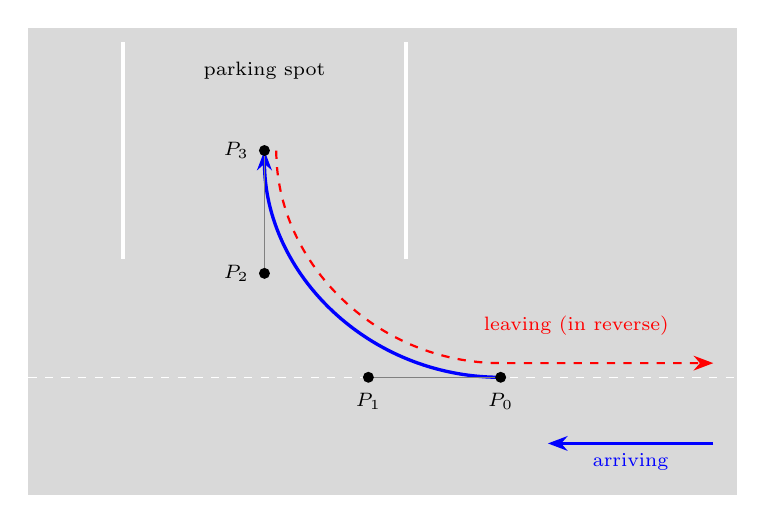
\begin{tikzpicture}[x=0.6cm,y=-0.6cm,pt/.style={circle,fill,inner sep=1.4pt},lab/.style={font=\scriptsize}]
\fill[gray!30] (-2,8.6) rectangle (13,18.5);
\foreach \x in {0,6} {\draw[white,line width=1.5pt] (\x,8.9)--(\x,13.5);}
\draw[white,dashed] (-2,16)--(13,16);
\node[lab] at (3,9.5) {parking spot};
\draw[very thick,blue,-{Stealth[length=2.5mm]}] (8,16) .. controls (5.2,16) and (3,13.8) .. (3,11.2);
\draw[thick,red,dashed,-{Stealth[length=2.5mm]}] (3.25,11.2) .. controls (3.25,13.6) and (5.4,15.7) .. (8,15.7) -- (12.5,15.7);
\draw[gray] (8,16)--(5.2,16); \draw[gray] (3,13.8)--(3,11.2);
\node[pt,label={[lab]below:$P_0$}] at (8,16) {};
\node[pt,label={[lab]below:$P_1$}] at (5.2,16) {};
\node[pt,label={[lab]left:$P_2$}] at (3,13.8) {};
\node[pt,label={[lab]left:$P_3$}] at (3,11.2) {};
\draw[arr,blue] (12.5,17.4) -- (9,17.4) node[midway,below,lab]{arriving};
\node[lab,red] at (9.6,14.9) {leaving (in reverse)};
\end{tikzpicture}
\caption{Parking (blue, forward) and leaving (red, reverse) curves for one spot.}
\end{figure}
The speed is limited by the place (9 m/s on the road, 4 m/s in the lot, 1.8 m/s while parking, 1.3 m/s in reverse) and
by the remaining distance $s_{left}$ with a braking deceleration of $2.2\,\mathrm{m/s^2}$:
\[
v\le\sqrt{2\cdot2.2\cdot s_{left}}+0.25 .
\]
A car stops when another car is less than 7.5 m ahead in its lane or a person is less than 5.5 m ahead. Only the car
holding the \emph{lot token} may park or unpark; cars in the aisle wait while it moves, and a car only starts to
reverse when the aisle behind it is clear. These two rules prevent deadlocks.

\subsection{Indoor navigation and activities}
Inside the building visitors walk on a waypoint graph of 18 nodes and 22 edges (doorways, room centres, the queue
at the ATM). The shortest route is found with \textbf{Dijkstra's algorithm}: starting from the nearest node, the
node $u$ with the smallest known distance is taken and its neighbours are relaxed,
\[
d(v) \leftarrow \min\big(d(v),\ d(u) + |\mathbf{x}_u-\mathbf{x}_v|\big),
\]
until the goal is reached; the route is then read back through the predecessors. People walk at 1.35 m/s and
wait when someone blocks the way. Every visitor has a plan of 1--3 activities, and each activity first
\emph{reserves} its resource (a machine, a seat, a reading place), so two people never use the same thing:
\begin{itemize}
  \item \textbf{Vending}: walk to a machine, press the keys (pressing pose), wait for the drop, bend down, take the
        item and carry it. This runs the machine's own state machine.
  \item \textbf{Coffee}: choose a drink, wait, take the cup and carry it.
  \item \textbf{ATM}: a complete ATM session; the ATM presses its own buttons with short pauses, so the screen shows
        every step.
  \item \textbf{Watch TV} (7 sofa seats) or \textbf{read} (2 library armchairs) for 12--28 s.
  \item \textbf{Browse books} or \textbf{watch the fish}.
\end{itemize}
A machine that the player is using is not available to visitors.
\begin{figure}[H]
\centering
\begin{subfigure}{0.49\linewidth}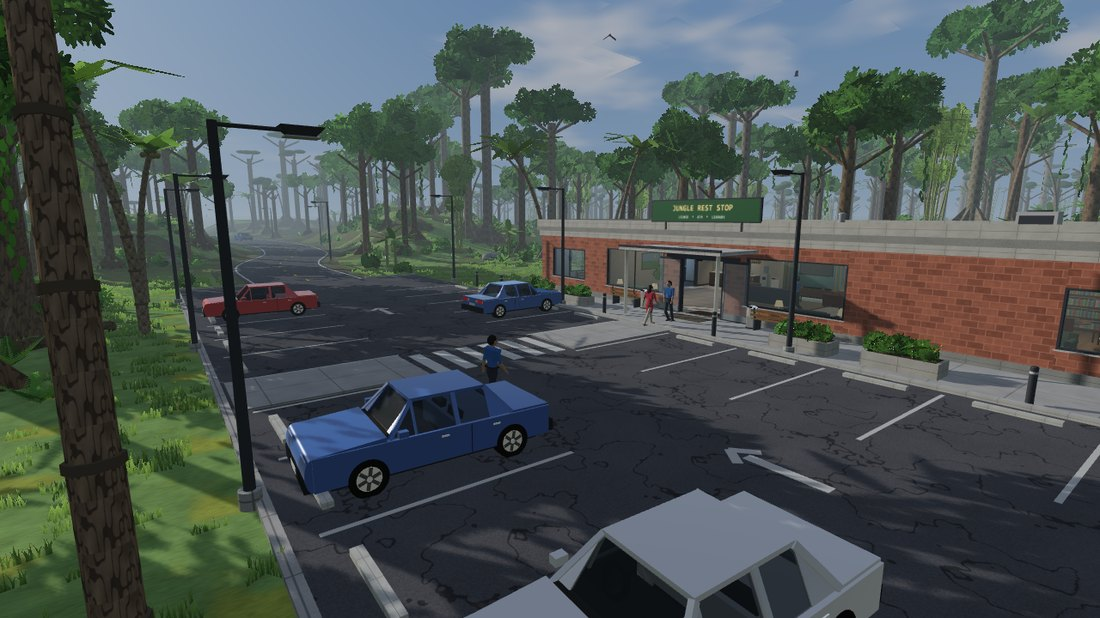
\includegraphics[width=\linewidth]{parking_lot}\caption{Parked cars and a visitor walking to the entrance}\end{subfigure}
\begin{subfigure}{0.49\linewidth}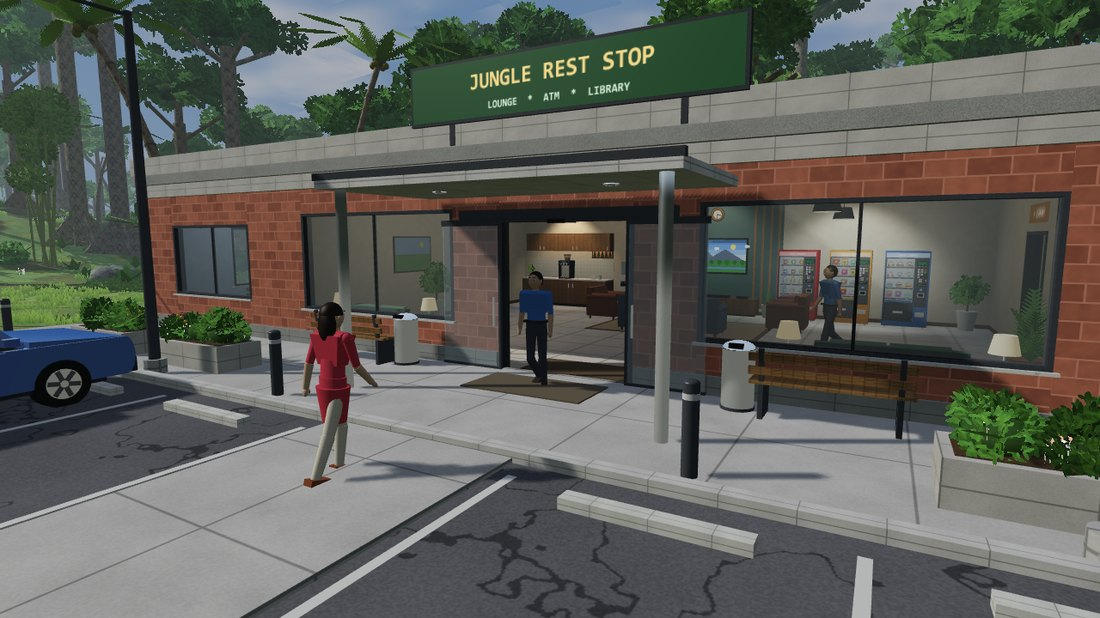
\includegraphics[width=\linewidth]{story_enter}\caption{Walking in through the sliding doors}\end{subfigure}
\begin{subfigure}{0.49\linewidth}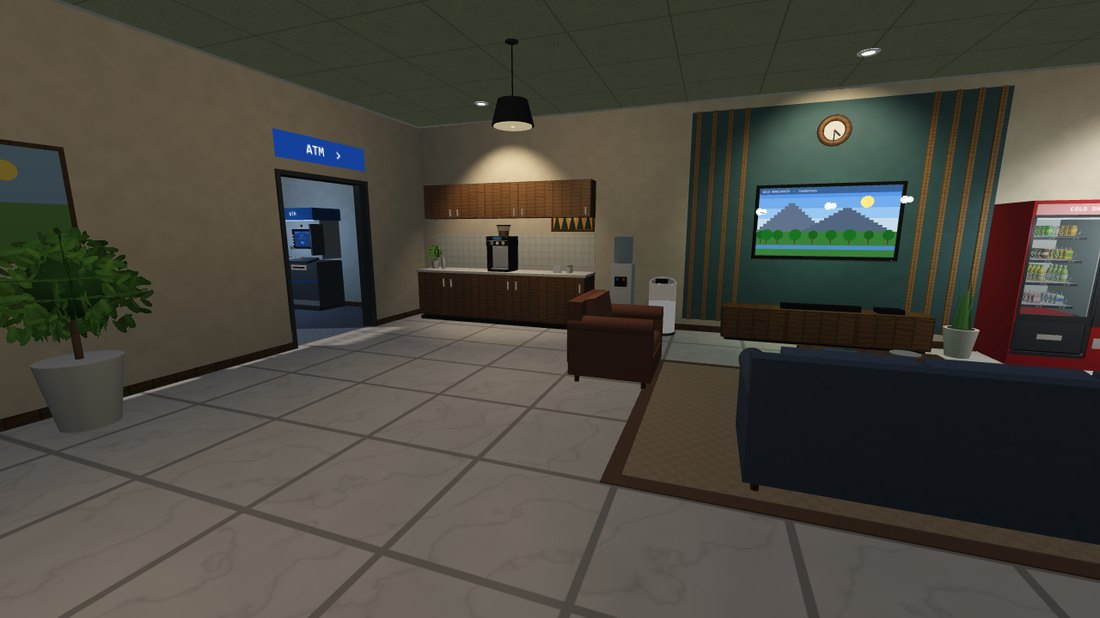
\includegraphics[width=\linewidth]{visitors_inside}\caption{Watching TV (the TV light falls on them)}\end{subfigure}
\begin{subfigure}{0.49\linewidth}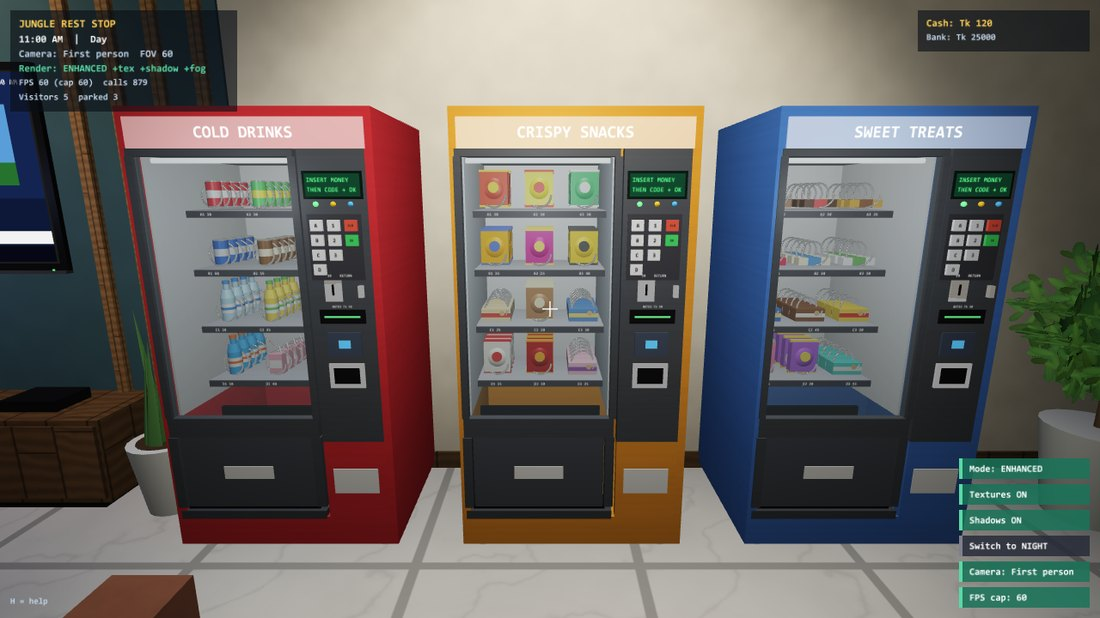
\includegraphics[width=\linewidth]{vending_row}\caption{Buying from a vending machine}\end{subfigure}
\caption{NPC visitors.}\label{fig:visitors}
\end{figure}
\Cref{lst:trace} shows the beginning of a trace recorded by the program.
\lstinputlisting[language={},caption={Start of a visitor trace (simulation time, visitor, spot, activity)},label={lst:trace},basicstyle=\ttfamily\scriptsize]{generated/visitor_trace.txt}

% =============================================================================
\section{Animation, Particles, Text and Sound}\label{sec:effects}
\subsection{Autonomous behaviour}
Every moving character is a state machine plus a simple movement rule (\Cref{tab:ai}).
\begin{table}[H]
\centering\small
\caption{Characters that move on their own}\label{tab:ai}
\begin{tabularx}{\linewidth}{@{}P{2.2cm}P{4.0cm}X@{}}
\toprule
Who & Decision (what to do) & Movement (how) \\ \midrule
Visitor & state machine with reserved resources (\Cref{fig:visitorsm}) & Dijkstra route on the waypoint graph, 1.35 m/s, waits when blocked \\
Car & part of the visitor's state machine; lot token & path following by length $s$, Bézier parking, braking limit $v\le\sqrt{2as_{left}}$ \\
Fish & swim; swim up while there is food & ellipse $x=r_x\cos\varphi$, $z=r_z\sin\varphi$, heading $\operatorname{atan2}(\Delta x,\Delta z)$ \\
Birds & fly by day & circles $\mathbf{p} = \mathbf{c} + (r\cos a,\ h + 1.5\sin 2a,\ r\sin a)$, $a \mathrel{+}= \omega\Delta t$ \\
Fireflies & appear at night, outdoors & drift on sine curves around the camera \\
\bottomrule
\end{tabularx}
\end{table}
\paragraph{Fish.} The height of a fish moves slowly towards $y_{target} = y_0 + 0.03\sin(0.7t+\varphi)$ at no more than
0.25 m/s; while there is food, $y_{target}$ is the water surface. The tail wags with $R_y(25^\circ\sin(9t+3\varphi))$.
\paragraph{Birds.} The wings are boxes in child nodes rotated by $R_z(\pm35^\circ\sin(\text{flap}))$ with
$\text{flap} \mathrel{+}= 9\,\Delta t$.
\paragraph{Fireflies.} 110 glowing spheres whose positions are wrapped into a $60\times60$ m box around the camera,
$x' = ((x - x_{cam}) \bmod 60) - 30 + x_{cam}$, so some are always near the viewer. Each blinks with
$0.5+0.5\sin(3t+3\varphi)$ and is hidden below 0.25.

\subsection{Particles}\label{sec:particles}
A particle is a small basic shape with a position $\mathbf{p}$, a velocity $\mathbf{v}$ and a life time. Every frame
$\mathbf{v} \mathrel{+}= \mathbf{g}\,\Delta t$ (for falling particles), $\mathbf{p} \mathrel{+}= \mathbf{v}\,\Delta t$ and the life decreases
by $\Delta t$; at the end of its life the particle is removed.
\begin{table}[H]
\centering\small
\caption{Particle effects}\label{tab:particles}
\begin{tabularx}{\linewidth}{@{}P{2.6cm}P{2.6cm}X@{}}
\toprule
Effect & Shape & Rule \\ \midrule
Coffee steam & transparent sphere & a new puff every 0.12 s while brewing; rises 7 cm/s and sways; grows from 2 to 6 cm; $\alpha = 0.25\cdot\text{life}$; lives 1.6 s \\
Change coins & thin cylinder & fall with $g=9.81\ \mathrm{m/s^2}$ into the coin cup \\
Falling product & the product & gravity, spin and a bounce $v_y \leftarrow -0.32\,v_y$ \\
Aquarium bubbles & transparent sphere & rise 12--22 cm/s with a wobble; restart at the bottom \\
Fish food & tiny sphere & sinks 4 cm/s, lives 5--8 s \\
Fireflies & glowing sphere & see above \\
\bottomrule
\end{tabularx}
\end{table}

\subsection{Text rendering}\label{sec:text}
All text (HUD, ATM and vending screens, TV, signs, price tags) uses one \textbf{font atlas}:
\begin{enumerate}
  \item At start-up Windows GDI draws the 95 printable ASCII characters (Consolas) into one bitmap, which becomes an
        OpenGL texture whose alpha channel is the shape of the letters.
  \item Each character is one textured quad (two triangles) whose texture coordinates select its cell in the atlas.
  \item \textbf{HUD text} uses the orthographic projection $\text{ortho}(0,W,H,0)$, so one unit is one pixel; depth
        testing is off, so it is always on top.
  \item \textbf{Text in the 3D world} is drawn on a \emph{canvas}: a flat rectangle with its own model matrix (for
        example the ATM screen). A canvas point $(x,y)$ is placed with
        $\mathbf{p} = M_{canvas}\,(x-\tfrac{w}{2},\ y-\tfrac{h}{2},\ 0,\ 1)^T$, so the text sits on the screen and turns
        with the machine. Depth testing is on, so a person in front hides the text.
\end{enumerate}
Text is blended with $C = \alpha\,C_{text} + (1-\alpha)\,C_{behind}$, which gives smooth letter edges.

\subsection{Sound}\label{sec:sound}
The sound uses 14 short recordings that are free to use (CC0, public domain; from Kenney.nl and OpenGameArt, listed
in \texttt{assets/sounds/CREDITS.txt}), stored as 44.1 kHz mono WAV files. The two background sounds (birds by day,
crickets at night) are loops whose end is cross-faded into their start. A mixer thread adds all playing sounds,
limits the sum with $\tanh$ and sends blocks of 2048 samples to the sound card with the Windows \texttt{waveOut}
functions. Sounds in the world become quieter with the distance $d$ from the camera,
\[
volume = \frac{v_0}{1+(d/4)^2},
\]
so a machine used by a visitor in another room is heard only faintly. The background is quieter inside the building.
\begin{table}[H]
\centering\small
\caption{Sounds}\label{tab:sounds}
\begin{tabularx}{\linewidth}{@{}P{3.0cm}X@{}}
\toprule
Sound & When \\ \midrule
click, beep & any button or switch; ATM keys; coffee ready \\
coin, thud, motor & vending: money in, change falling, product hitting the tray, spiral turning \\
cash, grinder, pouring & ATM gives money; coffee machine grinds and pours \\
door whoosh, car door & entrance doors start to move; a visitor opens or closes the car door \\
birds / crickets & quiet background loop by day / by night \\
\bottomrule
\end{tabularx}
\end{table}

% =============================================================================
\section{Performance}
\begin{itemize}
  \item \textbf{Instanced drawing}: all copies of one basic shape are drawn with one \texttt{glDrawElementsInstanced}
        call; each instance carries its model matrix, normal matrix, colour, emission, texture layer and material values.
  \item \textbf{Static world in chunks}: \statStaticInstances\ shapes that never move are collected once (in
        \statBuildSeconds\ s) into \statChunks\ chunks of $32\times32$ m, each with its own GPU buffer.
  \item \textbf{Culling}: a chunk is skipped when its bounding box is outside the view frustum (six planes taken from
        the view-projection matrix) or farther than 165 m. Grass and flowers end at 45 m, bushes, ferns and leaf cards at 85 m.
  \item \textbf{Occlusion culling}: visible chunks are drawn from near to far, and a chunk that was completely hidden in the
        previous frame (for example the jungle behind a wall) is skipped; only its bounding box is tested again with an
        occlusion query.
  \item \textbf{Depth pre-pass}: depth is written first with a minimal shader, then the lighting shader runs with
        \texttt{GL\_LEQUAL}, so every pixel is lit exactly once.
  \item \textbf{Per-room light lists}, frustum culling of lights, and a shadow pass that skips grass and glass.
  \item \textbf{Frame cap}: after each frame the program sleeps until $1/cap - 1.5$ ms and then waits the remaining time,
        which gives a steady 60 or 30 FPS.
\end{itemize}
\begin{table}[H]
\centering\small
\caption{Measured frame time without the frame cap (1280$\times$720, Intel Iris Xe)}
\begin{tabular}{l r r r r r}
\toprule
View & \multicolumn{2}{c}{Enhanced} & \multicolumn{2}{c}{Basic} & Triangles \\
 & ms & FPS & ms & FPS & (enh.) \\
\midrule
Outside, day & 14.0 & 72 & 10.8 & 93 & 2.25M \\
Main lounge & 11.7 & 86 & 8.3 & 120 & 2.25M \\
Inside the jungle & 10.2 & 98 & 8.3 & 121 & 1.87M \\
Parking lot, night & 11.7 & 86 & 11.2 & 90 & 1.64M \\
Aerial view & 15.3 & 66 & 12.9 & 78 & 2.16M \\
\bottomrule
\end{tabular}

\end{table}

% =============================================================================
\section{Conclusion}
Jungle Rest Stop is a small living world: three connected rooms with working machines, visitors who arrive by car and
act on their own, a dense jungle, and light that changes from morning to night. Every object is a set of basic shapes
placed with translation, rotation and scaling and organised in parent and child nodes. The project covers the main
topics of the course in one program: transformations and hierarchical modelling, viewing and projection,
illumination and shading, several light types, texture mapping, shadow mapping, fog, transparency, animation,
picking, collision detection and camera control, and it runs at a steady 60 FPS on integrated graphics.

% =============================================================================
\begin{thebibliography}{9}
\bibitem{red} J. Kessenich, G. Sellers, D. Shreiner. \emph{OpenGL Programming Guide}, 9th ed., Addison-Wesley, 2016.
\bibitem{lo} J. de Vries. \emph{Learn OpenGL}, \url{https://learnopengl.com} (lighting, shadow mapping, instancing).
\bibitem{hearn} D. Hearn, M. P. Baker, W. Carithers. \emph{Computer Graphics with OpenGL}, 4th ed., Pearson, 2010.
\bibitem{rtr} T. Akenine-M\"oller, E. Haines, N. Hoffman et al. \emph{Real-Time Rendering}, 4th ed., CRC Press, 2018.
\bibitem{blinn} J. F. Blinn. Models of light reflection for computer synthesized pictures. \emph{SIGGRAPH}, 1977.
\bibitem{williams} L. Williams. Casting curved shadows on curved surfaces. \emph{SIGGRAPH}, 1978.
\bibitem{perlin} K. Perlin. An image synthesizer. \emph{SIGGRAPH}, 1985.
\bibitem{glfw} GLFW documentation, \url{https://www.glfw.org}; GLAD loader, \url{https://glad.dav1d.de}.
\end{thebibliography}


\end{document}
